%                                                                             
%  MMO    MM   MMMMMM  MMMMMMM   MM    MMMMMMMM   MMD   MM  MMMMMMM MMMMMMM   
%  MMM   MMM   MM        MM     ?MMM              MMM$  MM  MM         MM     
%  MMMM 7MMM   MM        MM     MM8M    MMMMMMM   MMMMD MM  MM         MM     
%  MM MMMMMM   MMMMMM    MM    MM  MM             MM MMDMM  MMMMMM     MM     
%  MM  MM MM   MM        MM    MMMMMM             MM  MMMM  MM         MM     
%  MM     MM   MMMMMM    MM   MM    MM            MM   MMM  MMMMMMM    MM
%
%
%            - META-NET Language Whitepaper | Greek paper -
% 
% ----------------------------------------------------------------------------

\documentclass[]{../../metanetpaper}

\usepackage{multicol}

%!TEX TS-program = xelatex
\RequireXeTeX %Force XeTeX check

\usepackage{polyglossia}
\setotherlanguages{english,greek}

\title{Η Ελληνικη Γλωσσα στην Ψηφιακη Εποχη --- The Greek Language in the Digital Age}

\subtitle{White Paper Series --- Σειρά Λευκών Βίβλων}

\author{
  Maria Gavrilidou~ {\small R.\,C.~`Athena'/ILSP}\\
  Maria Koutsombogera~ {\small R.\,C.~`Athena'/ILSP}\\
  Anastasios Patrikakos~ {\small R.\,C.~`Athena'} \\
  Stelios Piperidis~ {\small R.\,C.~`Athena'/ILSP}
}
\editors{
  Georg Rehm, Hans Uszkoreit\\(επιμελητές, \textcolor{grey1}{editors})
}

\begin{document}

\maketitle

\null
\pagestyle{empty} 

\FundingLNotice{\selectlanguage{greek} Οι συντάκτες του κειμένου αυτού θα ήθελαν να ευχαριστήσουν τους συγγραφείς της γερμανικής λευκής βίβλου για την άδεια χρήσης επιλεγμένων εισαγωγικών χωρίων από το κείμενό τους \cite{lwpgerman}.

  \bigskip
  Η κατάρτιση αυτής της Λευκής Βίβλου χρηματοδοτήθηκε από το 7ο Πρόγραμμα Πλαίσιο και το Πρόγραμμα 'Υποστήριξη της Πολιτικής για τις ΤΠΕ' της Ευρωπαϊκής Επιτροπής, με τα Έργα Τ4ΜΕ (αρ.~σύμβασης: 249119), CESAR (αρ.~σύμβασης: 271022), METANET4U (αρ.~σύμβασης: 270893) και META-NORD (αρ.~σύμβασης: 270899).}

\FundingRNotice{\selectlanguage{english} The authors of this document
  are grateful to the authors of the White Paper on German for
  permission to re-use selected language-independent materials from
  their document \cite{lwpgerman}.
  
  \bigskip
  The development of this white paper has been funded by the Seventh
  Framework Programme and the ICT Policy Support Programme of the
  European Commission under the contracts T4ME (Grant Agreement
  249119), CESAR (Grant Agreement 271022), METANET4U (Grant Agreement
  270893) and META-NORD (Grant Agreement 270899).}

\makefundingnotice

\pagenumbering{Roman} 
\setcounter{page}{5}
\pagestyle{scrheadings}

\cleardoublepage

% --------------------------------------------------------------------------

\bsection*{Προοίμιο --- Preface}

\begin{Parallel}[c]{78mm}{78mm}
\ParallelLText{\selectlanguage{greek}
Η παρούσα Λευκή Βίβλος εντάσσεται σε μια σειρά από παρόμοιες ενημερωτικές αναφορές σχετικά με τη γλωσσική τεχνολογία και τις δυνατότητές της. Απευθύνεται σε εκπαιδευτικούς, δημοσιογράφους, πολιτικούς, γλωσσικές κοινότητες και άλλους φορείς. Η διαθεσιμότητα και η χρήση γλωσσικής τεχνολογίας στην Ευρώπη ποικίλλει από γλώσσα σε γλώσσα. Κατά συνέπεια, οι δράσεις που απαιτούνται για την περαιτέρω στήριξη της έρευνας και της ανάπτυξης γλωσσικών τεχνολογιών επίσης διαφέρουν σε κάθε γλώσσα. Οι απαιτούμενες δράσεις εξαρτώνται από πολλούς παράγοντες, όπως είναι η πολυπλοκότητα μιας γλώσσας και το μέγεθος της κοινότητάς της.

Το META-NET, ένα Δίκτυο Αριστείας που χρηματοδοτείται από την Ευρωπαϊκή Επιτροπή, διεξήγαγε μια  έρευνα των τρεχουσών γλωσσικών πόρων και τεχνολογιών (σελ.~\pageref{whitepaperseries}). Αυτή η έρευνα επικεντρώθηκε στις 23 επίσημες ευρωπαϊκές γλώσσες, καθώς και σε άλλες σημαντικές εθνικές και περιφερειακές γλώσσες στην Ευρώπη. Τα αποτελέσματα αυτής της ανάλυσης δείχνουν ότι υπάρχουν πολλά σημαντικά ερευνητικά κενά σε κάθε γλώσσα. Μια πιο λεπτομερής ανάλυση και εκτίμηση της τρέχουσας κατάστασης από εμπειρογνώμονες θα βοηθήσει στη μεγιστοποίηση των επιδράσεων της πρόσθετης έρευνας και στην ελαχιστοποίηση τυχόν κινδύνων.

Από το Νοέμβριο του 2011, το META-NET απαρτίζεται από 54 ερευνητικά κέντρα από 33 χώρες (σελ.~\pageref{metanetmembers}), και συνεργάζεται με φορείς που κυμαίνονται από εμπορικές επιχειρήσεις, δημόσιες υπηρεσίες, τη βιομηχανία, ερευνητικά ιδρύματα, εταιρείες ανάπτυξης λογισμικού, μέχρι εταιρείες παροχής τεχνολογίας και ευρωπαϊκά πανεπιστήμια. Όλοι μαζί οι φορείς υλοποιούν ένα κοινό τεχνολογικό όραμα ενώ αναπτύσσουν μια στρατηγική ατζέντα για την έρευνα που δείχνει πώς οι εφαρμογές γλωσσικής τεχνολογίας μπορούν να αντιμετωπίσουν οποιαδήποτε ερευνητικά κενά έως το 2020.}

\ParallelRText{\selectlanguage{english}
This white paper is part of a series that promotes knowledge about language technology and its potential. It addresses journalists, politicians, language communities, educators and others. 
The availability and use of language technology in Europe varies between languages. Consequently, the actions that are required to further support research and development of language technologies also differ. The required actions depend on many factors, such as the complexity of a given language and the size of its community.

META-NET, a Network of Excellence funded by the European Commission, has conducted an  analysis of current language resources and technologies in this white paper series (p.~\pageref{whitepaperseries}). The analysis focused on the 23 official European languages as well as other important national and regional languages in Europe. The results of this analysis suggest that there are tremendous deficits in technology support and significant research gaps for each language. The given detailed expert analysis and assessment of the current situation will help maximise the impact of additional research.

As of November 2011, META-NET consists of 54 research centres from 33 European countries (p.~\pageref{metanetmembers}). META-NET is working with stakeholders from economy (software companies, technology providers and users), government agencies, research organisations, non-governmental organisations, language communities and European universities. Together with these communities, META-NET is creating a common technology vision and strategic research agenda for multilingual Europe 2020.} 
\ParallelPar
\end{Parallel}

\cleardoublepage

% --------------------------------------------------------------------------
\bsection*{Περιεχόμενα --- Contents}

\selectlanguage{english}
\renewcommand\contentsname{}
\tableofcontents

\addtocontents{toc}{\protect\thispagestyle{empty}\protect}
\addtocontents{toc}{{\protect\vspace*{-10mm}\protect}}
\addtocontents{toc}{{\Large\textsf{\centerline{Η ΕΛΛΗΝΙΚΗ ΓΛΩΣΣΑ ΣΤΗΝ ΨΗΦΙΑΚΗ ΕΠΟΧΗ}}\par}}

\cleardoublepage

% --------------------------------------------------------------------------
\setcounter{page}{1}
\pagenumbering{arabic} 
\pagestyle{scrheadings}

% Start of origin language part
% --------------------------------------------------------------------------
\ssection[Περίληψη]{Περίληψη}

\selectlanguage{greek}

\begin{multicols}{2}
 \selectlanguage{greek}
Τα τελευταία 60 χρόνια, παρόλο που η Ευρώπη έχει γίνει μια σαφής πολιτική και οικονομική οντότητα, εντούτοις παρουσιάζει έντονη πολιτισμική και γλωσσική ποικιλότητα. Αυτό σημαίνει ότι, από τα πορτογαλικά έως τα πολωνικά και από τα ιταλικά έως τα ισλανδικά, η επικοινωνία μεταξύ των Ευρωπαίων πολιτών σε καθημερινό αλλά και σε επιχειρηματικό και πολιτικό επίπεδο παρεμποδίζεται αναπόφευκτα από γλωσσικούς φραγμούς. Οι οργανισμοί της Ευρωπαϊκής Ένωσης δαπανούν ετησίως περίπου ένα δις για τη διατήρηση της πολιτικής της πολυγλωσσίας, ήτοι τη μετάφραση κειμένων και τη διερμηνεία της προφορικής επικοινωνίας. Ωστόσο, γιατί πρέπει αυτό να αποτελεί  επιβάρυνση; Η σύγχρονη γλωσσική τεχνολογία και η γλωσσολογική έρευνα μπορούν να συνεισφέρουν σημαντικά στην κατάργηση των γλωσσικών φραγμών. Ο συνδυασμός της γλωσσικής τεχνολογίας με έξυπνες συσκευές και εφαρμογές θα παρέχει μελλοντικά στους Ευρωπαίους τη δυνατότητα συνομιλίας και επιχειρηματικών συναλλαγών μεταξύ τους ακόμη και αν δεν μιλούν την ίδια γλώσσα. 

\boxtext{Η γλωσσική τεχνολογία χτίζει γέφυρες\\ για το μέλλον της Ευρώπης.}

Οι γλωσσικοί φραγμοί θέτουν εμπόδια στην ανάπτυξη των επιχειρήσεων, κυρίως των μικρομεσαίων, οι οποίες δεν διαθέτουν τα οικονομικά μέσα για να αντιστρέψουν την κατάσταση. Η μόνη (αδιανόητη) εναλλακτική λύση θα ήταν η υιοθέτηση μίας μόνο γλώσσας, η οποία θα είχε κυρίαρχη θέση και τελικά θα αντικαθιστούσε όλες τις άλλες γλώσσες.

Ένας από τους παραδοσιακούς τρόπους αντιμετώπισης των γλωσσικών φραγμών είναι η εκμάθηση ξένων γλωσσών. Χωρίς όμως τεχνολογική υποστήριξη, η αντιμετώπιση των 23 επίσημων γλωσσών των κρατών μελών της Ευρωπαϊκής Ένωσης καθώς και των 60 περίπου άλλων ευρωπαϊκών γλωσσών αποτελεί αξεπέραστο εμπόδιο για τους Ευρωπαίους πολίτες καθώς και για την οικονομία, την πολιτική διαβούλευση και την επιστημονική πρόοδο της Ευρώπης. 

Η λύση εντοπίζεται στην ανάπτυξη βασικών τεχνολογιών, οι  οποίες θα προσφέρουν στους ευρωπαϊκούς φορείς σημαντικά πλεονεκτήματα όχι μόνο εντός της ευρωπαϊκής κοινής αγοράς αλλά και στις εμπορικές σχέσεις με τρίτες χώρες, κυρίως με τις αναδυόμενες οικονομίες. Η επίτευξη του στόχου αυτού και η διατήρηση της πολιτισμικής και γλωσσικής ποικιλότητας της Ευρώπης προϋποθέτουν τη διεξαγωγή συστηματικής ανάλυσης των ιδιαιτεροτήτων όλων των ευρωπαϊκών γλωσσών καθώς και του επιπέδου ανάπτυξης υποστηρικτικής γλωσσικής τεχνολογίας για καθεμιά από αυτές.

Τα εργαλεία αυτόματης μετάφρασης και επεξεργασίας φωνής που διατίθενται στο εμπόριο απέχουν ακόμη αρκετά από αυτόν τον φιλόδοξο στόχο. Οι κυρίαρχοι παίκτες στο χώρο αυτό είναι κατεξοχήν ιδιωτικές κερδοσκοπικές εταιρίες με έδρα τη Βόρεια Αμερική. Ήδη από τα τέλη του 1970 η ΕΕ αντιλήφθηκε τη σπουδαιότητα της γλωσσικής τεχνολογίας στην πορεία προς την ευρωπαϊκή ενοποίηση και ξεκίνησε τη χρηματοδότηση των πρώτων της ερευνητικών προγραμμάτων, όπως το EUROTRA. Παράλληλα, συστάθηκαν εθνικά έργα τα οποία, αν και παρήγαγαν σημαντικά αποτελέσματα δεν οδήγησαν ποτέ σε συντονισμένες ευρωπαϊκές ενέργειες. Σε αντίθεση προς αυτές τις προσπάθειες επιλεκτικής χρηματοδότησης, άλλες πολύγλωσσες κοινωνίες όπως η Ινδία (22 επίσημες γλώσσες) και η Ν. Αφρική (11 επίσημες γλώσσες) έχουν οργανώσει μακροπρόθεσμα εθνικά προγράμματα γλωσσικής έρευνας και τεχνολογικής ανάπτυξης. 

Οι κυρίαρχοι παίκτες στο χώρο της γλωσσικής τεχνολογίας σήμερα βασίζονται σε μη ακριβείς στατιστικές προσεγγίσεις οι οποίες δεν αξιοποιούν γλωσσολογικές μεθόδους και γνώση. Για παράδειγμα, οι προτάσεις που μεταφράζονται αυτόματα  προκύπτουν από τη σύγκριση μιας νέας πρότασης με  χιλιάδες προτάσεις που έχουν προηγουμένως μεταφραστεί από ανθρώπους. Η ποιότητα του αποτελέσματος εξαρτάται σε μεγάλο βαθμό από το μέγεθος και την ποιότητα του διαθέσιμου σώματος κειμένων. Αν και η αυτόματη μετάφραση απλών προτάσεων σε γλώσσες με επαρκή όγκο διαθέσιμων πόρων μπορεί να επιτύχει ικανοποιητικά αποτελέσματα, οι επιφανειακές στατιστικές μέθοδοι τέτοιου τύπου είναι καταδικασμένες να αποτύχουν σε περιπτώσεις γλωσσών με πολύ μικρότερο σώμα δεδομένων ή σε περιπτώσεις προτάσεων με πολύπλοκες δομές.

\boxtext{Η γλωσσική τεχνολογία είναι\\ το κλειδί για το μέλλον.}

Η Ευρωπαϊκή Ένωση αποφάσισε να χρηματοδοτήσει έργα όπως το EuroMatrix και το EuroMatrixPlus (από το 2006) και το iTranslate4 (από το 2010), στο πλαίσιο των οποίων διεξάγεται βασική και εφαρμοσμένη έρευνα και παράγονται πόροι που εξασφαλίζουν λύσεις γλωσσικής τεχνολογίας υψηλής ποιότητας για όλες τις ευρωπαϊκές γλώσσες. Η ανάλυση των βαθύτερων δομικών ιδιοτήτων των γλωσσών  είναι η μόνη διέξοδος, αν ο στόχος είναι η ανάπτυξη εφαρμογών υψηλής απόδοσης για το συνολικό εύρος των ευρωπαϊκών γλωσσών. Η ευρωπαϊκή έρευνα στο χώρο αυτό έχει ήδη σημειώσει αρκετές επιτυχίες. Για παράδειγμα, οι μεταφραστικές υπηρεσίες της Ευρώπης χρησιμοποιούν πλέον το Moses, λογισμικό ανοιχτού κώδικα για την αυτόματη μετάφραση, το οποίο αναπτύχθηκε κυρίως στο πλαίσιο ευρωπαϊκών ερευνητικών προγραμμάτων. Αντί να αξιοποιεί τα αποτελέσματα των ευρωπαϊκών της προγραμμάτων, η Ευρώπη έχει την τάση να επιδιώκει μεμονωμένες ερευνητικές δράσεις  με περιορισμένο αντίκτυπο στην αγορά. Η οικονομική αξία ακόμη και των πρώιμων προσπαθειών είναι εμφανής και στην περίπτωση των τεχνοβλαστών, όπως  της εταιρίας Trados, η οποία ιδρύθηκε το 1984 και αγοράστηκε από την βρετανική SDL το 2005.

\boxtext{Η γλωσσική τεχνολογία συμβάλλει\\ στην ενοποίηση της Ευρώπης.}

Κρίνοντας από τα αποτελέσματα των εξελίξεων στο χώρο, φαίνεται πως η σημερινή ‘υβριδική’ γλωσσική τεχνολογία που συνδυάζει τη γλωσσική επεξεργασία με στατιστικές μεθόδους είναι σε θέση να γεφυρώσει το χάσμα μεταξύ των ευρωπαϊκών γλωσσών. Όπως φαίνεται και από την παρούσα σειρά των λευκών βίβλων, υπάρχουν σημαντικές διαφορές μεταξύ των κρατών μελών της Ευρώπης ως προς την ετοιμότητα της γλωσσικής τεχνολογίας και το επίπεδο της έρευνας. Αν και ο χώρος της γλωσσικής τεχνολογίας στην Ελλάδα έχει σημειώσει σημαντική πρόοδο τα τελευταία χρόνια, απαιτείται περαιτέρω έρευνα και ανάπτυξη για την επίτευξη πραγματικά αποτελεσματικών λύσεων γλωσσικής τεχνολογίας για καθημερινή χρήση. 

Μακροπρόθεσμο στόχο του ΜΕΤΑ-ΝΕΤ αποτελεί η σύσταση γλωσσικής τεχνολογίας υψηλής ποιότητας για όλες τις γλώσσες με στόχο την επίτευξη της πολιτικής και κοινωνικής ενοποίησης μέσω της πολιτισμικής ποικιλότητας. Η τεχνολογία θα βοηθήσει στην κατάργηση των υπαρχόντων φραγμών και θα δημιουργήσει γέφυρες μεταξύ των γλωσσών της Ευρώπης. Ο στόχος αυτός απαιτεί  την συνένωση των προσπαθειών όλων των εμπλεκόμενων φορέων στην πολιτική, την έρευνα, τις επιχειρήσεις και την κοινωνία.

Η συλλογή των εν λόγω λευκών βίβλων αποτελεί μια από της στρατηγικές δραστηριότητες που έχει αναλάβει το ΜΕΤΑ-ΝΕΤ (βλ. παράρτημα). Περαιτέρω ενημερώσεις σχετικά με τις εκδόσεις των σχετικών εγγράφων \cite{Meta1},  συμπεριλαμβανομένης της Στρατηγικής Ατζέντας για την Έρευνα, βρίσκονται στον ιστότοπο του ΜΕΤΑ-ΝΕΤ: http://www.meta-net.eu.
\end{multicols}

\clearpage

% --------------------------------------------------------------------------

\ssection[Γλώσσες σε κίνδυνο: μια Πρόκληση για τη Γλωσσική Τεχνολογία]{Γλώσσες σε κίνδυνο: μια Πρόκληση\newline για τη Γλωσσική Τεχνολογία}

\begin{multicols}{2}
 \selectlanguage{greek}
Είμαστε μάρτυρες μιας ψηφιακής επανάστασης η οποία επηρεάζει δραματικά την επικοινωνία και την κοινωνία. Οι πρόσφατες εξελίξεις στην ψηφιακή τεχνολογία των πληροφοριών και των επικοινωνιών αρκετές φορές συγκρίνονται με την εφεύρεση; της τυπογραφίας από τον Γουτεμβέργιο. Τι μας λέει αυτή η αναλογία για το μέλλον της ευρωπαϊκής κοινωνίας της πληροφορίας, και ειδικότερα για το μέλλον των γλωσσών μας;

\boxtext{Σήμερα είμαστε μάρτυρες μιας\\ ψηφιακής επανάστασης που μπορεί\\ να συγκριθεί με την εφεύρεση της\\ τυπογραφίας από τον Γουτεμβέργιο.}

Μετά την εφεύρεση του Γουτεμβέργιου επιτεύχθηκαν πραγματικές καινοτομίες στην επικοινωνία και την ανταλλαγή γνώσεων με προσπάθειες όπως η μετάφραση της Βίβλου στην καθομιλουμένη από τον Λούθηρο. Στους αιώνες που ακολούθησαν, αναπτύχθηκαν πολιτισμικές τεχνικές για την καλύτερη προσέγγιση της επεξεργασίας του λόγου και της ανταλλαγής γνώσεων:

\medskip
\begin{itemize}
\item Η ορθογραφική και γραμματική τυποποίηση ευρέως διαδεδομένων γλωσσών επέτρεψε την ταχεία διάδοση νέων επιστημονικών και πνευματικών ιδεών.
\item Η ανάπτυξη επίσημων γλωσσών κατέστησε δυνατή την επικοινωνία των πολιτών εντός ορισμένων (συχνά πολιτικών) συνόρων.
\item Η διδασκαλία και η μετάφραση γλωσσών επέτρεψε διαγλωσσικές ανταλλαγές.
\item Η δημιουργία εκδοτικών και βιβλιογραφικών οδηγιών διασφάλισε την ποιότητα και τη διαθεσιμότητα έντυπου υλικού.
\item Η δημιουργία διαφορετικών μέσων όπως οι εφημερίδες, το ραδιόφωνο, η τηλεόραση, τα βιβλία κ.\,ά.~ικανοποίησε διάφορες επικοινωνιακές ανάγκες.
\end{itemize}

Τα τελευταία είκοσι χρόνια, η πληροφορική έχει βοηθήσει στην αυτοματοποίηση και τη διευκόλυνση πολλών διαδικασιών:

\begin{itemize}
\item οι ηλεκτρονικές εκδόσεις έχουν αντικαταστήσει την δακτυλογράφηση και τη στοιχειοθεσία,
\item το Microsoft PowerPoint έχει αντικαταστήσει τον προβολέα διαφανειών,
\item το ηλεκτρονικό ταχυδρομείο στέλνει και λαμβάνει έγγραφα ταχύτερα και από το φαξ,
\item το Skype προσφέρει οικονομικές τηλεφωνικές κλήσεις μέσω Διαδικτύου και υποστηρίζει εικονικές συσκέψεις,
\item τα μορφότυπα κωδικοποίησης ήχου και βίντεο διευκολύνουν την ανταλλαγή πολυμεσικού περιεχομένου,
\item οι μηχανές αναζήτησης προσφέρουν πρόσβαση σε ιστοσελίδες βασιζόμενες σε λέξεις κλειδιά,
\item διαδικτυακές υπηρεσίες όπως το Google Translate παράγουν γρήγορες, κατά προσέγγιση μεταφράσεις,
\item οι πλατφόρμες κοινωνικής δικτύωσης όπως το Facebook, το Twitter και το Google+ διευκολύνουν την επικοινωνία, τη συνεργασία και την ανταλλαγή πληροφοριών.
\end{itemize}

Αν και αυτά τα εργαλεία και οι εφαρμογές είναι χρήσιμα, δεν είναι ακόμα ικανά να υποστηρίξουν μια βιώσιμη, πολυγλωσσική ευρωπαϊκή κοινωνία για όλους, όπου οι πληροφορίες και τα αγαθά θα μπορούν να διακινούνται ελεύθερα.

\subsection{Γλωσσικά σύνορα: εμπόδιο στην Ευρωπαϊκή Κοινωνία της Πληροφορίας}
  
Δεν είμαστε σε θέση να προβλέψουμε πώς ακριβώς θα μοιάζει η μελλοντική κοινωνία της πληροφορίας. Υπάρχει όμως μεγάλη πιθανότητα η επανάσταση στην τεχνολογία επικοινωνιών να φέρει κοντά ανθρώπους που μιλάνε διαφορετικές γλώσσες με νέους τρόπους. Το γεγονός αυτό ωθεί τους ανθρώπους προς την εκμάθηση νέων γλωσσών και, ασκεί πίεση στους προγραμματιστές, να δημιουργήσουν νέες τεχνολογικές εφαρμογές που να εξασφαλίζουν την αμοιβαία κατανόηση και την πρόσβαση σε διαμοιραζόμενες γνώσεις. Στην παγκόσμια οικονομία και στον παγκόσμιο χώρο πληροφοριών, περισσότερες γλώσσες, ομιλητές και περιεχόμενο αλληλεπιδρούν ταχύτερα με νέους τύπους μέσων. Η τρέχουσα δημοτικότητα των κοινωνικών μέσων (Wikipedia, Facebook, Twitter, YouTube, και προσφάτως το Google+) είναι μόνον η κορυφή του παγόβουνου.

\boxtext{Η παγκόσμια οικονομία και\\ ο ενιαίος χώρος πληροφοριών μας φέρνει αντιμέτωπους με περισσότερες γλώσσες, ομιλητές και περιεχόμενο.}

Σήμερα, μπορούμε να μεταδίδουμε gigabytes κειμένου σε ολόκληρο τον πλανήτη μέσα σε λίγα δευτερόλεπτα προτού αντιληφθούμε ότι αφορά μια γλώσσα που δεν κατανοούμε. Σύμφωνα με μια πρόσφατη έκθεση της Ευρωπαϊκής Επιτροπής, το 57\% των χρηστών του Ίντερνετ στην Ευρώπη αγοράζουν εμπορεύματα και υπηρεσίες χρησιμοποιώντας γλώσσες οι οποίες δεν είναι οι μητρικές τους (τα αγγλικά είναι η πιο διαδεδομένη ξένη γλώσσα κι ακολουθούν τα γαλλικά, τα γερμανικά και τα ισπανικά.) Το 55\% των χρηστών διαβάζει περιεχόμενο σε κάποια ξένη γλώσσα, ενώ μόλις το 35\% χρησιμοποιεί άλλη γλώσσα για να γράψει ηλεκτρονικά μηνύματα ή να κάνει σχόλια στο διαδίκτυο \cite{EC1}. Πριν από λίγα χρόνια, τα αγγλικά ίσως ήταν η lingua franca του διαδικτύου — η μεγάλη πλειονότητα του περιεχομένου στο διαδίκτυο ήταν στα αγγλικά — αλλά η κατάσταση έχει πλέον αλλάξει δραματικά. Η ποσότητα του διαδικτυακού περιεχομένου σε άλλες ευρωπαϊκές  γλώσσες (καθώς και σε ασιατικές και μεσανατολικές) έχει υπερπολλαπλασιαστεί. 

Προκαλεί έκπληξη το γεγονός ότι αυτό το πανταχού παρόν ψηφιακό χάσμα λόγω των γλωσσικών συνόρων δεν έχει προσελκύσει ιδιαίτερα την προσοχή,  παρόλο που θέτει ένα πολύ πιεστικό ερώτημα: ποιες ευρωπαϊκές γλώσσες θα κατορθώσουν να επιβιώσουν στη δικτυωμένη κοινωνία της πληροφορίας και της γνώσης και ποιες είναι καταδικασμένες να εξαφανιστούν;

\subsection{Οι γλώσσες μας κινδυνεύουν}

Παρόλο που η τυπογραφία βοήθησε στην ενίσχυση της ανταλλαγής πληροφοριών στην Ευρώπη, οδήγησε επίσης στον αφανισμό πολλών ευρωπαϊκών γλωσσών. Οι περιφερειακές και μειονοτικές γλώσσες σπανίως τυπώνονταν και γλώσσες όπως τα κορνουαλικά και τα δαλματικά περιορίστηκαν σε προφορικές μορφές μετάδοσης, οι οποίες με τη σειρά τους περιόρισαν το πεδίο χρήσης τους. Θα έχει και το διαδίκτυο τις ίδιες επιπτώσεις στις γλώσσες μας;

Οι κατά προσέγγιση 80 γλώσσες της Ευρώπης είναι ένα από τα πολυτιμότερα και σημαντικότερα πολιτιστικά της περιουσιακά στοιχεία, καθώς και ζωτικό κομμάτι του μοναδικού της κοινωνικού μοντέλου \cite{EC2}. Ενώ γλώσσες όπως τα αγγλικά και τα ισπανικά είναι πιθανότερο να επιβιώσουν στην αναδυόμενη ψηφιακή αγορά, πολλές ευρωπαϊκές γλώσσες θα μπορούσαν να αποβούν ήσσονος σημασίας σε μια διαδικτυωμένη κοινωνία. Αυτό θα αποδυνάμωνε την παγκόσμια θέση της Ευρώπης και θα εναντιωνόταν  στον στρατηγικό στόχο της διασφάλισης της ίσης συμμετοχής κάθε Ευρωπαίου πολίτη ανεξαρτήτως γλώσσας.

\boxtext{Η μεγάλη ποικιλία γλωσσών στην Ευρώπη είναι ένα από τα πολυτιμότερα και σημαντικότερα πολιτισμικά περιουσιακά της στοιχεία.}

Σύμφωνα με μια έκθεση της UNESCO για την πολυγλωσσία, οι γλώσσες αποτελούν ένα ουσιαστικό μέσο για την απόλαυση θεμελιωδών δικαιωμάτων, όπως η πολιτική έκφραση, η εκπαίδευση και η συμμετοχή στην κοινωνία \cite{Unesco1}.

\subsection{Γλωσσική Τεχνολογία: μια βασική τεχνολογία προσβασιμότητας}

Στο παρελθόν, οι επενδυτικές προσπάθειες για τη διατήρηση των γλωσσών επικεντρώνονταν στη γλωσσική εκπαίδευση και τη μετάφραση. Σύμφωνα με μια εκτίμηση, η ευρωπαϊκή αγορά μετάφρασης, διερμηνείας, λογισμικών τοπικοποίησης (localisation) και παγκοσμιοποίησης δικτυακών τόπων (website globalisation) ανερχόταν σε 8,4 δισεκατομμύρια € το 2008 και αναμένεται να αυξάνεται κατά 10\% ετησίως \cite{EC3}. Κι όμως αυτός ο αριθμός καλύπτει ένα πολύ μικρό ποσοστό των τρεχουσών και των μελλοντικών αναγκών διαγλωσσικής επικοινωνίας. Η πιο επιτακτική λύση για τη διασφάλιση του εύρους και του βάθους της χρήσης της γλώσσας στην Ευρώπη του αύριο είναι η χρήση της κατάλληλης τεχνολογίας, ακριβώς όπως χρησιμοποιούμε τεχνολογία για να λύσουμε, μεταξύ άλλων, τις ανάγκες μας για μεταφορά, ενέργεια και πρόσβαση.

Η γλωσσική τεχνολογία (που στοχεύει σε κάθε μορφή γραπτού κειμένου και προφορικού λόγου) βοηθά τους ανθρώπους να συνεργάζονται, να συναλλάσσονται, να μοιράζονται γνώσεις και να συμμετέχουν στον κοινωνικό και πολιτικό διάλογο ανεξάρτητα από γλωσσικούς φραγμούς και δεξιότητες χρήσης υπολογιστή. Συχνά λειτουργεί αόρατα μέσα σε σύνθετα συστήματα λογισμικού για να μας βοηθήσει:

\begin{itemize}
\item να βρούμε πληροφορίες με μια μηχανή αναζήτησης,
\item να ελέγξουμε την ορθογραφία και τη γραμματική σε έναν επεξεργαστή κειμένου,
\item να δούμε συστάσεις για προϊόντα σε ένα διαδικτυακό κατάστημα,
\item να ακούσουμε φωνητικές οδηγίες από ένα σύστημα πλοήγησης αυτοκινήτου,
\item να μεταφράσουμε ιστοσελίδες μέσω μιας διαδικτυακής υπηρεσίας. 
\end{itemize}

Η γλωσσική τεχνολογία απαρτίζεται από πολλές κεντρικές εφαρμογές που καθιστούν δυνατές διαδικασίες στο πλαίσιο μιας μεγαλύτερης εφαρμογής. Ο στόχος των λευκών βίβλων του META-NET για τη γλώσσα είναι να εστιάσουν στο πόσο έτοιμες είναι αυτές οι κεντρικές τεχνολογίες για κάθε ευρωπαϊκή γλώσσα. 

\boxtext{Η Ευρώπη χρειάζεται αξιόπιστη\\ και οικονομική γλωσσική τεχνολογία\\ για όλες τις ευρωπαϊκές γλώσσες.}

Για να διατηρήσουμε τη θέση μας στην πρώτη γραμμή της παγκόσμιας καινοτομίας, η Ευρώπη θα χρειαστεί γλωσσική τεχνολογία προσαρμοσμένη σε όλες τις ευρωπαϊκές γλώσσες, η οποία θα είναι αξιόπιστη, οικονομική και σωστά  ολοκληρωμένη σε βασικά περιβάλλοντα λογισμικού. Χωρίς γλωσσική τεχνολογία δεν θα κατορθώσουμε στο προσεχές μέλλον να προσφέρουμε μια πραγματικά αποτελεσματική, διαδραστική, πολυμεσική και πολυγλωσσική εμπειρία στο χρήστη.

\subsection{Ευκαιρίες για τη Γλωσσική Τεχνολογία}

Στον κόσμο της τυπογραφίας, τεχνολογική καινοτομία αποτέλεσε η γρήγορη αναπαραγωγή μιας εικόνας ενός κειμένου (σελίδας) χρησιμοποιώντας ένα κατάλληλο μηχανοκίνητο τυπογραφικό πιεστήριο. Άνθρωποι καλούνταν να επιτελέσουν το δύσκολο έργο της έρευνας, του διαβάσματος, της μετάφρασης και της συνοπτικής παρουσίασης της γνώσης. Χρειάστηκε να περιμένουμε μέχρι τον Έντισον για να καταγράψουμε τον προφορικό λόγο – και πάλι η τεχνολογία του απλά παρήγαγε αναλογικά αντίγραφα.

Η γλωσσική τεχνολογία μπορεί πλέον να αυτοματοποιήσει τις ίδιες τις διεργασίες της μετάφρασης, της παραγωγής περιεχομένου και της διαχείρισης γνώσης για όλες τις ευρωπαϊκές γλώσσες. Μπορεί επίσης να εμπλουτίσει οικιακά ηλεκτρονικά συστήματα, μηχανήματα, οχήματα, υπολογιστές και ρομπότ με διεπαφές βασισμένες σε γραπτό ή προφορικό λόγο. Οι εμπορικές και βιομηχανικές εφαρμογές βρίσκονται ακόμη σε αρχικά στάδια ανάπτυξης, αλλά τα επιτεύγματα της Ε\&Α δημιουργούν πραγματικές ευκαιρίες. Για παράδειγμα, η μηχανική μετάφραση είναι ήδη σχετικά ακριβής σε συγκεκριμένους τομείς. Επίσης, υπάρχουν πειραματικές εφαρμογές που προσφέρουν πολυγλωσσικές πληροφορίες και διαχείριση γνώσης, καθώς και παραγωγή περιεχομένου σε πολλές ευρωπαϊκές γλώσσες.

Όπως συμβαίνει με τις περισσότερες τεχνολογίες, οι πρώτες γλωσσικές εφαρμογές όπως οι φωνητικές διεπαφές χρήστη και τα διαλογικά συστήματα αναπτύχθηκαν για πολύ εξειδικευμένους τομείς, και συχνά παρουσιάζουν περιορισμένη απόδοση. Υπάρχουν όμως τεράστιες επιχειρηματικές ευκαιρίες στον τομέα της εκπαίδευσης και της ψυχαγωγίας σχετικά με την ολοκλήρωση γλωσσικών τεχνολογιών σε παιχνίδια, χώρους πολιτιστικής κληρονομιάς, ψυχαγωγικά εκπαιδευτικά πακέτα, βιβλιοθήκες, περιβάλλοντα προσομοίωσης και προγράμματα επιμόρφωσης. Υπηρεσίες ενημέρωσης κινητής τηλεφωνίας, λογισμικό εκμάθησης γλωσσών μέσω Η/Υ, περιβάλλοντα εξ αποστάσεως μάθησης, εργαλεία αυτο-αξιολόγησης και λογισμικό εντοπισμού λογοκλοπής είναι μόνο μερικοί από τους τομείς εφαρμογής όπου η γλωσσική τεχνολογία μπορεί να διαδραματίσει σημαντικό ρόλο. Η δημοτικότητα των εφαρμογών κοινωνικών μέσων όπως το Twitter και το Facebook δείχνουν μια περαιτέρω ανάγκη για προηγμένες γλωσσικές τεχνολογίες που να μπορούν να παρακολουθούν τις αναρτήσεις, να συνοψίζουν συζητήσεις, να αναδεικνύουν τις τάσεις της κοινής γνώμης, να ανιχνεύουν συγκινησιακές αντιδράσεις, να εντοπίζουν παραβιάσεις πνευματικών δικαιωμάτων ή να ανιχνεύουν παράνομες χρήσεις.

\boxtext{Η γλωσσική τεχνολογία βοηθά στην\\ υπέρβαση της 'αναπηρίας' που\\ επιφέρει η γλωσσική ποικιλότητα.} 

Η γλωσσική τεχνολογία αποτελεί τεράστια ευκαιρία για την Ευρωπαϊκή Ένωση. Μπορεί να βοηθήσει στην αντιμετώπιση του σύνθετου ζητήματος της πολυγλωσσίας στην Ευρώπη – το γεγονός ότι διαφορετικές γλώσσες συνυπάρχουν φυσικά σε ευρωπαϊκές επιχειρήσεις, οργανισμούς και σχολεία. Αλλά οι πολίτες χρειάζεται να επικοινωνούν υπερπηδώντας τα γλωσσικά σύνορα, καθώς διασχίζουν από άκρη σε άκρη την Ευρωπαϊκή Κοινή Αγορά, και η γλωσσική τεχνολογία μπορεί να βοηθήσει στην υπέρβαση αυτού του τελευταίου φραγμού, υποστηρίζοντας παράλληλα την ελεύθερη και απρόσκοπτη χρήση των διαφόρων γλωσσών. Κοιτάζοντας ακόμα πιο μπροστά, η καινοτόμος ευρωπαϊκή πολύγλωσση γλωσσική τεχνολογία θα αποτελέσει σημείο αναφοράς για τους παγκόσμιους εταίρους μας, όταν θα ξεκινήσουν να οργανώνουν τις δικές τους πολύγλωσσες κοινότητες. Η γλωσσική τεχνολογία μπορεί να ιδωθεί ως μια μορφή 'υποστηρικτικής' τεχνολογίας που βοηθά στην υπέρβαση της 'αναπηρίας' της γλωσσικής ποικιλότητας και κάνει τις γλωσσικές κοινότητες πιο προσβάσιμες τη μία στην άλλη.

Τέλος, ένα δυναμικό πεδίο έρευνας είναι η χρήση της γλωσσικής τεχνολογίας σε επιχειρήσεις διάσωσης σε περιοχές καταστροφών, όπου το ζήτημα της επίδοσης μπορεί να είναι ζήτημα ζωής και θανάτου: μελλοντικά ευφυή ρομπότ με διαγλωσσικές ικανότητες έχουν τη δυνατότητα να σώζουν ζωές.

\subsection{Προκλήσεις που αντιμετωπίζει η Γλωσσική Τεχνολογία}

Αν και η γλωσσική τεχνολογία έχει σημειώσει σημαντική πρόοδο τα τελευταία χρόνια, ο τρέχων ρυθμός τεχνολογικής προόδου και καινοτομίας είναι πολύ αργός. Ευρέως διαδεδομένες τεχνολογίες όπως οι ορθογραφικοί και γραμματικοί διορθωτές σε κειμενογράφους είναι συνήθως μονόγλωσσοι και είναι διαθέσιμοι μόνο για λίγες γλώσσες.

\boxtext{Ο τρέχων ρυθμός της τεχνολογικής\\ προόδου είναι πολύ αργός.}

Οι διαδικτυακές υπηρεσίες μηχανικής μετάφρασης, παρ' ότι είναι σε θέση να παραγάγουν σχετικά αποδεκτή προσέγγιση του περιεχομένου ενός εγγράφου, βρίθουν προβλημάτων, όταν απαιτούνται μεταφράσεις υψηλής ακρίβειας και πληρότητας. Εξαιτίας της πολυπλοκότητας της ανθρώπινης γλώσσας, η μοντελοποίηση των γλωσσών μας και η δοκιμή του μοντέλου στον πραγματικό κόσμο είναι μια μακρά, δαπανηρή υπόθεση που απαιτεί δεσμεύσεις συνεχούς χρηματοδότησης. Η Ευρώπη πρέπει επομένως να διατηρήσει τον πρωτοποριακό της ρόλο στην αντιμετώπιση των τεχνολογικών προκλήσεων μιας πολύγλωσσης κοινότητας επινοώντας νέες μεθόδους για την επιτάχυνση της ανάπτυξης από τη μία άκρη του χάρτη ως την άλλη. Αυτές θα μπορούσαν να περιλαμβάνουν τόσο τις εξελίξεις στην επιστήμη των υπολογιστών όσο και τεχνικές όπως είναι ο πληθοπορισμός (crowdsourcing).

\subsection{Κατάκτηση της γλώσσας από ανθρώπους και μηχανήματα}

Για να απεικονίσουμε το πώς οι υπολογιστές χειρίζονται τη γλώσσα και γιατί είναι δύσκολο να τους προγραμματίσουμε ώστε να την χρησιμοποιούν, ας ρίξουμε μια γρήγορη ματιά στον τρόπο που οι άνθρωποι μαθαίνουν την πρώτη και τη δεύτερη γλώσσα, κι έπειτα θα εξετάσουμε το πώς λειτουργούν τα συστήματα γλωσσικής τεχνολογίας.

\boxtext{Ο άνθρωπος κατακτά γλωσσικές δεξιότητες με δύο διαφορετικούς τρόπους: μαθαίνοντας παραδείγματα και μαθαίνοντας τους υποκείμενους γλωσσικούς κανόνες.}

Οι άνθρωποι κατακτούν γλωσσικές δεξιότητες με δύο διαφορετικούς τρόπους. Τα μωρά μαθαίνουν μια γλώσσα ακούγοντας τους γονείς τους, τα αδέρφια τους και άλλα μέλη της οικογένειάς τους να μιλάνε σε πραγματικές συνθήκες. Από την ηλικία περίπου των δύο ετών, τα παιδιά λένε τις πρώτες τους λέξεις και σχηματίζουν μικρές φράσεις. Αυτό είναι εφικτό μόνο επειδή ο άνθρωπος έχει γενετική προδιάθεση να μιμείται κι έπειτα να εκλογικεύει τα όσα ακούει. 

Η εκμάθηση μιας δεύτερης γλώσσας σε μεγαλύτερη ηλικία απαιτεί μεγαλύτερη προσπάθεια, κυρίως επειδή το παιδί δεν περιβάλλεται από μια γλωσσική κοινότητα φυσικών ομιλητών. Στο σχολείο, οι ξένες γλώσσες συνήθως διδάσκονται μέσω  γραμματικής, λεξιλογίου και ορθογραφίας με τη χρήση ασκήσεων που περιγράφουν τη γλωσσική γνώση εκπεφρασμένη σε αφηρημένους κανόνες, πίνακες και παραδείγματα. 

Οι δύο κύριοι τύποι συστημάτων γλωσσικής τεχνολογίας 'κατακτούν' γλωσσικές ικανότητες με παρόμοιο τρόπο. Οι στατιστικές προσεγγίσεις (ή 'βασισμένες σε δεδομένα') αποκτούν γλωσσική γνώση από τεράστιες συλλογές δειγμάτων πραγματωμένου λόγου. Ενώ αρκεί η χρήση κειμένου σε μια μόνον γλώσσα για την εκπαίδευση, π.\,χ.~ενός ορθογράφου, απαιτούνται παράλληλα κείμενα σε δύο (ή περισσότερες) γλώσσες για την εκπαίδευση ενός συστήματος μηχανικής μετάφρασης. Ο  αλγόριθμος μηχανικής μάθησης 'μαθαίνει' τρόπους μετάφρασης λέξεων, σύντομων φράσεων και ολόκληρων προτάσεων. 

Αυτή η στατιστική προσέγγιση απαιτεί εκατομμύρια προτάσεων και η ποιότητα της επίδοσής του  αυξάνεται ανάλογα με την όγκο των κειμένων που έχει αναλύσει. Αυτός είναι ο λόγος για τον οποίο οι πάροχοι των μηχανών αναζήτησης ενδιαφέρονται να συγκεντρώσουν όσο περισσότερο γραπτό υλικό μπορούν. Ο ορθογραφικός έλεγχος σε κειμενογράφους αλλά και υπηρεσίες όπως το Google Search και το Google Translate  βασίζονται σε στατιστικές προσεγγίσεις. Το μεγάλο πλεονέκτημα της στατιστικής είναι ότι η μηχανή μαθαίνει γρήγορα μέσα από διαρκείς σειρές αλλεπάλληλων κύκλων εκμάθησης, αν και η ποιότητά τους μπορεί να ποικίλλει.

Η δεύτερη προσέγγιση της γλωσσικής τεχνολογίας και συγκεκριμένα της μηχανικής μετάφρασης είναι η δημιουργία συστημάτων βασισμένων σε κανόνες. Ειδικοί στους τομείς της γλωσσολογίας, της υπολογιστικής γλωσσολογίας και της πληροφορικής πρώτα καλούνται να κωδικοποιήσουν γραμματικές αναλύσεις (κανόνες μετάφρασης) και να συγκεντρώσουν καταλόγους λεξιλογίου (λεξικά). Αυτό είναι εξαιρετικά χρονοβόρο και απαιτεί εντατική εργασία. Ορισμένα από τα καλύτερα συστήματα μηχανικής μετάφρασης βάσει κανόνων αναπτύσσονται εδώ και πάνω από μία εικοσαετία. Το μεγάλο πλεονέκτημα των συστημάτων αυτών είναι ότι οι ειδικοί έχουν ουσιαστικό έλεγχο στην επεξεργασία της γλώσσας. Αυτό δίνει τη δυνατότητα να διορθώνονται συστηματικά τα λάθη στο λογισμικό και να υπάρχει αναλυτικός σχολιασμός προς το χρήστη, ειδικά όταν συστήματα βασισμένα σε κανόνες χρησιμοποιούνται για την εκμάθηση γλώσσας. Εξαιτίας, ωστόσο, του υψηλού κόστους αυτής της διαδικασίας, η βασισμένη σε  κανόνες τεχνολογία προς το παρόν έχει αναπτυχθεί μόνο για τις μεγάλες γλώσσες. 

Καθώς τα πλεονεκτήματα και οι αδυναμίες των στατιστικών και των βασισμένων σε κανόνες συστημάτων τείνουν να αλληλοσυμπληρώνονται, η  έρευνα εστιάζει πλέον σε υβριδικές προσεγγίσεις που συνδυάζουν τις δύο μεθοδολογίες. Εντούτοις, αυτές οι προσεγγίσεις μέχρι σήμερα ήταν λιγότερο πετυχημένες σε βιομηχανικές εφαρμογές από ό,τι στο ερευνητικό εργαστήριο. 

Όπως είδαμε σε αυτό το κεφάλαιο, πολλές ευρέως διαδεδομένες εφαρμογές στη σημερινή κοινωνία της πληροφορίας βασίζονται σε πολύ μεγάλο βαθμό στη γλωσσική τεχνολογία. Εξαιτίας της πολύγλωσσης κοινότητάς της, αυτό ισχύει ιδιαίτερα για την οικονομία και την τεχνολογία της Ευρώπης. Αν και η γλωσσική τεχνολογία έχει σημειώσει σημαντική πρόοδο τα τελευταία λίγα χρόνια, υπάρχουν ακόμα τεράστιες δυνατότητες για βελτίωση της ποιότητας των συστημάτων γλωσσικής τεχνολογίας. Ακολούθως, θα περιγράψουμε το ρόλο των ελληνικών στην ευρωπαϊκή κοινωνία της πληροφορίας και θα κάνουμε μια εκτίμηση της σημερινής κατάστασης της γλωσσικής τεχνολογίας για την ελληνική γλώσσα.
\end{multicols}

\clearpage

% --------------------------------------------------------------------------
\ssection[Τα ελληνικά στην ευρωπαϊκή κοινωνία της πληροφορίας]{Τα ελληνικά στην ευρωπαϊκή \newline κοινωνία της πληροφορίας}

\begin{multicols}{2}
\selectlanguage{greek}
\subsection{Γενικά δεδομένα}

Τα ελληνικά είναι η επίσημη γλώσσα της Ελλάδας και μία από τις δύο επίσημες γλώσσες της Κύπρου και από το 1981 μία από τις επίσημες γλώσσες της Ευρωπαϊκής Ένωσης. Ομιλείται ως μητρική γλώσσα από περίπου το 95\% από τα 11,5 εκατομμύρια κατοίκους της Ελλάδας και από περίπου 500.000 Ελληνοκυπρίους \cite{Stat1}. Χρησιμοποιείται επίσης (σε διαφορετικά επίπεδα γλωσσομάθειας)  από συνολικά περίπου 5 εκατομμύρια ανθρώπους ελληνικής καταγωγής, μέλη ελληνικών κοινοτήτων (τη λεγόμενη Διασπορά) παγκοσμίως \cite{Dias1}, πρωτίστως στις ΗΠΑ, την Αυστραλία (η Μελβούρνη αποκαλείται 'η τρίτη μεγαλύτερη ελληνική πόλη στον κόσμο'), τον Καναδά, την Ευρώπη (κυρίως τη Βρετανία και τη Γερμανία), τις χώρες της πρώην Σοβιετικής Ένωσης, την Τουρκία και την Αίγυπτο.

Τα ελληνικά είναι Ινδοευρωπαϊκή γλώσσα, το μοναδικό σωζόμενο μέλος του ελληνικού κλάδου της οικογένειας των Ινδοευρωπαϊκών γλωσσών \cite{Trud1}. Σε αντίθεση με τα Λατινικά, από τα οποία γεννήθηκαν αρκετές θυγατρικές γλώσσες, ο μοναδικός απόγονος της  Αρχαίας Ελληνικής είναι η σύγχρονη Ελληνική. Έχει την πιο μακρόχρονη τεκμηριωμένη ιστορία από όλες τις Ινδοευρωπαϊκές γλώσσες, καλύπτοντας 34 αιώνες γραπτών μνημείων.

Μετά την Κλασική Αρχαιότητα, από τον 4ο αιώνα π.\,Χ.~κι έπειτα, οι διάφορες διάλεκτοι υπέστησαν ισοπέδωση, και δημιουργήθηκε μια οικουμενική διάλεκτος, η \textit{Κοινή} (κοινή γλώσσα), η οποία σε μεγάλο βαθμό βασιζόταν στην Αττική διάλεκτο εμπλουτισμένη με στοιχεία από άλλες διαλέκτους. Αυτή η κοινή γλώσσα ομιλούνταν, ως μητρική ή ως δεύτερη γλώσσα, σε μια γεωγραφική περιοχή  που εκτεινόταν γύρω από τη Μεσόγειο. Η βασική ελληνόφωνη επικράτεια, στο  νότιο τμήμα της βαλκανικής χερσονήσου, που εκτεινόταν στα δυτικά έως τη Νότια Ιταλία και τη Σικελία και στα ανατολικά έως τη Μικρά Ασία, κάποιες εποχές απέκτησε σημαντικές διαστάσεις (Αίγυπτος, Εγγύς Ανατολή, Ανατολία κ.\,λπ.) και ήρθε σε επαφή με πολλούς πολιτισμούς και γλώσσες. Σημειώθηκε εκτενής απλοποίηση της γλώσσας αναφορικά με τη μορφολογία, τη σύνταξη και το λεξιλόγιο, και τα Ελληνικά έγιναν μια ευρέως ομιλούμενη \textit{lingua franca}. Στα βυζαντινά χρόνια (μετά το 610 μ.Χ.), καθιερώθηκε ως επίσημη γλώσσα της Βυζαντινής Αυτοκρατορίας.

Σχεδόν όλες οι ποικιλίες της σύγχρονης Ελληνικής προέρχονται από την \textit{Κοινή} \cite{Bro1}. Μετά τον Β' Παγκόσμιο Πόλεμο, οι διάφορες ελληνικές διάλεκτοι σταδιακά παράκμασαν και μερικές (π.\,χ.~η καππαδοκική διάλεκτος, η Τσακώνικη, η Γκρίκο, η ελληνική διάλεκτος που ομιλείται σε μερικά χωριά της Νοτίου Ιταλίας, περιοχή γνωστή επίσης και ως Μεγάλη Ελλάδα) θεωρείται ότι έχουν σχεδόν εξαφανιστεί. Οι διάλεκτοι που υπάρχουν σήμερα θεωρούνται περισσότερο στοιχεία πολιτιστικής ταυτότητας, καθώς ομιλούνται αποκλειστικά μεταξύ των μελών  των συγκεκριμένων κοινοτήτων. Ο σύγχρονος τρόπος ζωής, η αστικοποίηση, η χρήση της πρότυπης ποικιλίας στην εκπαίδευση και τα μέσα ενημέρωσης έχουν οδηγήσει στην υποχώρησή τους έναντι της πρότυπης Νέας Ελληνικής. Τέτοιες διάλεκτοι των ελληνικών είναι η ποντιακή, η κυπριακή και η κρητική διάλεκτος. 

\subsection{Το ελληνικό αλφάβητο}

Το ελληνικό σύστημα γραφής είναι το ελληνικό αλφάβητο κατά το μεγαλύτερο μέρος της ιστορίας του. Παλαιότερα χρησιμοποιούνταν άλλα συστήματα \cite{Kopi1}. Το ελληνικό αλφάβητο δημιουργήθηκε με βάση το φοινικικό αλφάβητο (κατά τον Ηρόδοτο), δηλαδή το σημιτικό αλφάβητο, το οποίο χρησιμοποιούσε σύμβολα για να παραστήσει μόνο σύμφωνα. Το ελληνικό αλφάβητο εισήγαγε – ή μάλλον επαναχρησιμοποίησε υφιστάμενα σύμβολα που δεν αντιστοιχούσαν σε ελληνικά φωνήματα για να παραστήσει τα φωνήεντα. Αυτό το αλφάβητο χρησιμοποιείται περίπου από τον 10ο αιώνα π.\,Χ.~\cite{Tonn1}, και αποτέλεσε τη βάση του Λατινικού, του Κυριλλικού, του Κοπτικού και πολλών άλλων συστημάτων γραφής.

Κατά την κλασική εποχή, υπήρχαν μόνο κεφαλαία γράμματα. Κατά τα ελληνιστικά χρόνια, εισήχθησαν διακριτικά σημάδια και τόνοι προκειμένου να εξηγούν τον τρόπο προφοράς συγκεκριμένων φωνηέντων, δεδομένου ότι η προσωδία είχε αλλάξει. Αυτά τα διακριτικά σημάδια καθιερώθηκαν στο γραφηματικό  σύστημα της Ελληνικής \cite{Chris1}. Τα πεζά γράμματα αναπτύχθηκαν πολύ αργότερα, από γραφείς του Μεσαίωνα.

Το σύγχρονο ελληνικό αλφάβητο απαρτίζεται από 24 γράμματα. Η μεταρρύθμιση της γραφής το 1982 κατάργησε τα διακριτικά σημάδια. Έκτοτε, η επίσημη ορθογραφία της Ελληνικής είναι το απλοποιημένο \textit{μονοτονικό} σύστημα, που χρησιμοποιεί μόνο τον τόνο και τα διαλυτικά. Το παραδοσιακό \textit{πολυτονικό} σύστημα συνεχίζει να χρησιμοποιείται διεθνώς για τη γραφή των Αρχαίων Ελληνικών.

Ιστορικά, η χρήση του λατινικού αλφάβητου για την αναπαράσταση της ελληνικής γλώσσας έχει διαπιστωθεί, π.\,χ.~σε περιοχές οι οποίες τέλεσαν υπό βενετσιάνικη κατοχή ή από Έλληνες Καθολικούς. Προσφάτως, η χρήση του λατινικού αλφαβήτου για τη γραφή Ελληνικών αποτελεί μια τάση που παρατηρείται κυρίως σε μηνύματα ηλεκτρονικού ταχυδρομείου και γραπτά μηνύματα μέσω κινητών τηλεφώνων. Αυτή η γραφή καλείται 'Greeklish'.

\boxtext{Διγλωσσία}

Η Ελλάδα απέκτησε την ανεξαρτησία της το 1830 (ήταν πολύ μικρότερη σε σχέση με σήμερα). Ο πυρήνας της νεοϊδρυθείσας χώρας ήταν η Αθήνα και η Πελοπόννησος. Κατά συνέπεια, οι διάλεκτοι που ομιλούνταν σε αυτές τις περιοχές αποτέλεσαν τη βάση για τη δημιουργία της πρότυπης ποικιλίας της Ελληνικής γλώσσας (της νόρμας).  Εντούτοις, η εξέλιξη της γλώσσας δεν ήταν απρόσκοπτη: σημειώθηκε εκτενής γλωσσικός προγραμματισμός υπό την επιρροή του ιδανικού της εθνικής γλώσσας του Διαφωτισμού. Σύμφωνα με την Δενδρινού \cite{Dend1},"οι αρχαϊστές υποστήριζαν την αναβίωσης της αρχαίας Ελληνικής, απαλλαγμένης από "ακάθαρτες" προσμίξεις που την είχαν 'μολύνει' στις διάφορες επαφές της". Η άλλη πλευρά ήταν υπέρμαχος της χρήσης της καθομιλουμένης γλώσσας του λαού, ενώ μια τρίτη άποψη υποστήριζε ένα μείγμα των δύο, συγκεκριμένα τη χρήση της σύγχρονης γλώσσας, 'καθαρισμένης' μέσα από την πρόσμιξη με την αρχαία ελληνική μορφολογία, σύνταξη και λεξιλόγιο. Επικράτησε η τρίτη άποψη, η οποία έφερε επίσης το συμβολικό φορτίο της συνέχισης της Αρχαίας Ελληνικής, με συνέπεια μια μακρά περίοδο διγλωσσίας.

Η διγλωσσία, δηλαδή η ταυτόχρονη ύπαρξη μιας καθομιλουμένης και μιας υψηλής ποικιλίας, ήταν στο προσκήνιο από τη γέννηση του νέου κράτους έως ουσιαστικά τα τέλη του 20ού αιώνα. Η λόγια ποικιλία, η  \textit{Καθαρεύουσα}, μια απομίμηση των αρχαίων Ελληνικών, χρησιμοποιούνταν σε όλους τους τομείς του δημόσιου βίου (πολιτική, διοίκηση, εκπαίδευση, επιστήμη) ενώ η λαϊκή ποικιλία, η  \textit{Δημοτική}, χρησιμοποιούνταν στην καθημερινή ανεπίσημη επικοινωνία, τη λογοτεχνία (αν και όχι από όλους τους συγγραφείς) και την πρωτοβάθμια εκπαίδευση.

Το πρόβλημα της διγλωσσίας έληξε επισήμως το 1976, όταν η Δημοτική ανακηρύχθηκε επίσημη γλώσσα της Ελλάδας. Σήμερα, η απόσταση ανάμεσα στη Δημοτική και την Καθαρεύουσα μικραίνει, καθώς η πρότυπη ελληνική γλώσσα η οποία χρησιμοποιείται για όλους τους επίσημους και ανεπίσημους σκοπούς συνδυάζει πτυχές και των δύο.

\subsection{Ιδιαιτερότητες της ελληνικής γλώσσας}

Τα Ελληνικά είναι μια γλώσσα με πλούσιο κλιτικό σύστημα, με τέσσερις πτώσεις για το ονοματικό σύστημα, τρία γένη και δύο αριθμούς \cite{Mack1}. Τα Ελληνικά έχουν έναν εκτενή  αριθμό  παραγωγικών παραθημάτων, ενώ το σύστημα της σύνθεσης είναι σχετικά περιορισμένο αλλά παραγωγικό. Κατά την εξέλιξη της γλώσσας μέσα στους αιώνες, οι μορφολογικές κατηγορίες διατηρήθηκαν σχετικά σταθερές. Η μεγαλύτερη αλλαγή στη μορφολογία του ονοματικού συστήματος ήταν η απώλεια της δοτικής πτώσης (τις λειτουργίες της οποίας ανέλαβαν σε μεγάλο βαθμό η γενική ή οι εμπρόθετες φράσεις). Στο ρήμα, η μεγάλη αλλαγή ήταν η απώλεια του απαρεμφάτου με την ταυτόχρονη ανάπτυξη νέων περιφραστικών τύπων.

\boxtext{Πολλά γλωσσικά χαρακτηριστικά της ελληνικής γλώσσας αποτελούν προκλήσεις για την υπολογιστική επεξεργασία.}

Το πλούσιο κλιτικό σύστημα προκαλεί συγκεκριμένες δυσκολίες σε συστήματα ΓΤ: η λημματοποίηση, για παράδειγμα, αντιμετωπίζει το περιβόητο πρόβλημα της αναγνώρισης ορισμένων κλιτικών τύπων που μπορεί να ανήκουν σε ένα ρήμα ή το ρηματικό ουσιαστικό του. Μια τέτοια περίπτωση ομογραφίας, για παράδειγμα, είναι η λέξη \textit{διαβάσεις}, που μπορεί να είναι

\begin{itemize}
\item δεύτερο πρόσωπο ενικού συνοπτικού ποιού ενεργείας του ρήματος \textit{διαβάζω} ή
\item ονομαστική ή αιτιατική πληθυντικού του ουσιαστικού \textit{η διάβαση}
\end{itemize}

Σε τέτοιες περιπτώσεις, τη λύση δίνει η επεξεργασία του περικειμένου.

Όσον αφορά στη σύνταξη, η χρήση των σωζόμενων πτώσεων έχει σε μεγάλο βαθμό διατηρηθεί ακέραιη (ονομαστική για υποκείμενα και κατηγορούμενα, αιτιατική για αντικείμενα των περισσοτέρων ρημάτων και πολλών προθέσεων, γενική για τα κτητικά), τα άρθρα προηγούνται των ουσιαστικών. Η απώλεια της δοτικής οδήγησε στη δημιουργία εμπρόθετων έμμεσων αντικειμένων (τα οποία εναλλακτικά  δηλώνονταν και με τη γενική). Η σειρά των λέξεων στα Ελληνικά είναι ελεύθερη και η ουδέτερη σειρά των όρων είναι Ρήμα-Υποκείμενο-Αντικείμενο ή Υποκείμενο-Ρήμα-Αντικείμενο. Αυτό επιτρέπει στους ομιλητές να σχηματίζουν εκφωνήματα με ποικίλους τρόπους και να βάζουν την έμφαση σε διάφορα μέρη της πρότασης. Ταυτόχρονα, αυτές οι παραλλαγές δημιουργούν και μεγάλες προκλήσεις για την υπολογιστική επεξεργασία φυσικής γλώσσας. Ας δούμε, για παράδειγμα, την αγγλική πρόταση

\begin{itemize}
\item[] The woman gave the man an apple.
\end{itemize}

Στα αγγλικά υπάρχουν δύο ακόμα τρόποι να εκφράσει κανείς την ίδια ιδέα, συγκεκριμένα:

\begin{itemize}
\item The woman gave an apple to the man.
\item An apple was given to the man by the woman.
\end{itemize}

Στα ελληνικά, η πρόταση αυτή θα μπορούσε να έχει την εξής δομή:

\begin{itemize}    
\item Η γυναίκα έδωσε στον άντρα ένα μήλο.
\item Η γυναίκα έδωσε ένα μήλο στον άντρα.
\item Έδωσε ένα μήλο η γυναίκα στον άντρα.
\item Έδωσε η γυναίκα ένα μήλο στον άντρα.
\item Έδωσε στον άντρα η γυναίκα ένα μήλο.
\item Στον άντρα έδωσε η γυναίκα ένα μήλο.
\item Στον άντρα έδωσε ένα μήλο η γυναίκα.
\item Ένα μήλο δόθηκε από τη γυναίκα στον άντρα.
\item Ένα μήλο δόθηκε στον άντρα από τη γυναίκα.
\item Δόθηκε ένα μήλο από τη γυναίκα στον άντρα.
\item Δόθηκε από τη γυναίκα στον άντρα ένα μήλο.
\item Δόθηκε στον άντρα ένα μήλο από τη γυναίκα.
\end{itemize}

Το πλούσιο κλιτικό σύστημα καθιστά την ελεύθερη σειρά των όρων της πρότασης εφικτή και προσφέρει πολύτιμες πληροφορίες στη συντακτική ανάλυση: η ονομαστική πτώση χρησιμοποιείται μόνο για υποκείμενα, και η αιτιατική για τα αντικείμενα των περισσότερων ρημάτων και πολλών προθέσεων, η γενική για τα κτητικά και τα αντικείμενα ορισμένων ρημάτων και προθέσεων. Κατά συνέπεια, η αναγνώριση των συντακτικών ρόλων είναι πιο απλή από ό,τι σε γλώσσες χωρίς πτώσεις. Επίσης, δεν είναι αναγκαίες οι αυστηρές θέσεις μέσα στην πρόταση για τους διάφορους συντακτικούς ρόλους.  
Τα Ελληνικά είναι μια γλώσσα με δυνατότητα παράλειψης των προσωπικών αντωνυμιών (pro-drop), όταν αυτές υποδηλώνονται μορφολογικά ή πραγματολογικά. Τη διαδικασία αναγνώρισης της παραλειπόμενης αντωνυμίας βοηθά το γεγονός ότι τα ρήματα περιλαμβάνουν ένα μόρφημα του προσώπου το οποίο συμφωνεί με την αντωνυμία ως προς το πρόσωπο και τον αριθμό. Συνήθως, οι προσωπικές αντωνυμίες 1ου και 2ου προσώπου του ενικού παραλείπονται (\textit{εγώ}, \textit{εσύ}). Η παρουσία τους υποδηλώνει έμφαση. Επομένως, η αγγλική πρόταση

\begin{itemize}
\item[] I am leaving.
\end{itemize}

μπορεί να αποδοθεί στα Ελληνικά ως

\begin{itemize}
\item Φεύγω. (ουδέτερη διατύπωση) ή 
\item Εγώ φεύγω. (έμφαση στο 'εγώ')
\end{itemize}

Δύο σημαντικά χαρακτηριστικά του ελληνικού λεξιλογίου είναι η έκτασή του και το μήκος των λέξεων. Μια αιτία για τον όγκο του λεξιλογίου είναι ο μεγάλος αριθμός συνωνύμων που παρατηρείται. Η πληθώρα συνωνύμων οφείλεται στην προέλευσή τους από τις διάφορες διαλέκτους, καθώς και από την Καθαρεύουσα (την λόγια ποικιλία). Όπως συμβαίνει με όλες τις γλώσσες, το λεξιλόγιο περιλαμβάνει επίσης λέξεις δανεισμένες από άλλες γλώσσες. Κατά συνέπεια, για την ίδια έννοια, είναι πιθανό να υπάρχουν 3 ή 4 λέξεις, καθεμιά προερχόμενη από μια διαφορετική γλώσσα. Στις περισσότερες περιπτώσεις, έχει επικρατήσει η λέξη της νόρμας της σύγχρονης Ελληνικής.

Μια άλλη αιτία για το εκτενές λεξιλόγιο είναι ο πλούτος του παραγωγικού μορφολογικού συστήματος: η παραγωγική αλυσίδα \textit{ρήμα} > \textit{ρηματικό ουσιαστικό} > \textit{ονοματικό επίθετο} > \textit{επίρρημα} είναι πολύ συνηθισμένη (π.\,χ.~δημιουργώ > δημιουργία/δημιουργός > δημιουργικός > δημιουργικά). Επίσης, τα Ελληνικά χαρακτηρίζονται από έναν ισχυρό παραγωγικό μηχανισμό για τα υποκοριστικά και τα μεγεθυντικά για ουσιαστικά και επίθετα.

Όσον αφορά το μήκος των λέξεων, τα Ελληνικά έχουν ελάχιστες μονοσύλλαβες λέξεις. Οι δισύλλαβες ή τρισύλλαβες λέξεις αποτελούν την πλειονότητα, αλλά οι πολυσύλλαβες λέξεις δεν είναι καθόλου σπάνιες (ακόμα και λέξεις με οκτώ ή εννιά συλλαβές).

Το λεξιλόγιο της Ελληνικής προέρχεται πρωτίστως από τα Αρχαία Ελληνικά είτε ως ατόφιες λέξεις (αν και κάποιες έχουν αλλάξει μορφολογικά ή σημασιολογικά) είτε ως ρίζες που παράγουν νέες λέξεις.

Σε παλαιότερες εποχές, δάνειες λέξεις προς τα Ελληνικά απέκτησαν ελληνικές καταλήξεις, κι έτσι προσαρμόστηκαν/ αφομοιώθηκαν στο μορφολογικό σύστημα. Σύγχρονα δάνεια (που εισήχθησαν κατά τις τελευταίες δεκαετίες), ειδικά από τα αγγλικά και τα γαλλικά, συνήθως δεν κλίνονται. Η απουσία κλιτικών μορφημάτων στη γλώσσα προέλευσης έχει ως αποτέλεσμα τη δυσκολία απόδοσης γένους, το οποίο ένα απαραίτητο χαρακτηριστικό γνώρισμα των ονομάτων. Παράγοντες που επηρεάζουν την απόδοση γένους είναι το αρχικό γένος (εάν υπάρχει), ο αναλογικός σχηματισμός (κατ' αναλογία με υπάρχουσες ελληνικές λέξεις) και η ομοιότητα (λέξεις που λήγουν σε κάποιο μόρφημα χαρακτηριστικό ενός συγκεκριμένου γένους θα αποδοθούν σε αυτό το γένος).

\subsection{Πρόσφατες εξελίξεις}

Από τη δεκαετία του 1950 κι έπειτα, οι αμερικανικές ταινίες άρχισαν να δεσπόζουν στην ελληνική αγορά. Η κυριαρχία ήταν ακόμα περισσότερο εμφανής κατά τη δεκαετία του 1970, όταν εισήχθησαν τηλεοπτικές σειρές σε κάθε νοικοκυριό. Οι ξένες ταινίες και οι τηλεοπτικές σειρές δεν μεταγλωττίζονται στην Ελλάδα. Αντίθετα, χρησιμοποιείται ο υποτιτλισμός (σε αντίθεση με πολλές άλλες χώρες όπως η Γαλλία και η Γερμανία). Η ισχυρή παρουσία του αμερικανικού τρόπου ζωής στα ΜΜΕ επηρέασε την ελληνική κουλτούρα και γλώσσα. Εξαιτίας της  συνεχούς επικράτησης της αγγλικής και αμερικανικής μουσικής από τη δεκαετία του 1960 και μετά, οι Έλληνες έχουν εκτεθεί πολύ στα αγγλικά στη διάρκεια της εφηβείας τους επί σειρά γενεών. Τα αγγλικά σύντομα απέκτησαν το καθεστώς της μοντέρνας, 'τρέντι' γλώσσας, το οποίο διατηρούν μέχρι και σήμερα. 

Αυτό το καθεστώς αντικατοπτρίζεται από τον τεράστιο αριθμό των σημερινών δανείων από τα Αγγλικά (τους λεγόμενους αγγλισμούς). Στις περισσότερες περιπτώσεις, αυτές οι λέξεις καλύπτουν κάποιο κενό στο λεξιλόγιο, π.\,χ.~ονομάζουν μια νέα ιδέα ή αντικείμενο για το οποίο δεν υφίσταται ελληνικό όνομα.

Εντούτοις, σε ορισμένες περιοχές, οι αγγλισμοί έχουν αρχίσει να αντικαθιστούν υφιστάμενο ελληνικό λεξιλόγιο. Ένα παράδειγμα είναι η χρήση αγγλικών τίτλων σε αγγελίες εργασίας, ιδιαίτερα για θέσεις διοικητικών στελεχών, π.\,χ.~`Human Resource Manager' αντί \textit{Υπεύθυνος Προσωπικού}. Επίσης, αγγλικά ονόματα καταστημάτων, επωνυμίες προϊόντων κ.\,λπ.~θεωρούνται περισσότερο 'πιασάρικα' από τα Ελληνικά. Τάση υπερβολικής χρήσης αγγλισμών μπορεί επίσης να διαπιστωθεί σε διαφημίσεις προϊόντων. Αυτή η τάση, όμως, όσο 'κουλ' κι αν φαντάζει, διατρέχει τον κίνδυνο να αποκλείει μεγάλα τμήματα του πληθυσμού από το να συμμετέχουν στην κοινωνία της πληροφορίας, και συγκεκριμένα, αυτούς που δεν γνωρίζουν αγγλικά.

\subsection{Γλωσσική πολιτική στην Ελλάδα}

Η Ελλάδα έχει ακολουθήσει διάφορες πολιτικές  στη διάρκεια του 20ού αιώνα σε μια προσπάθεια να ξεπεράσει το γλωσσικό πρόβλημα που κατέτρυχε τις απόπειρες Γλωσσικού Προγραμματισμού του διευρυνόμενου Ελληνικού Κράτους. 

Το ζήτημα της Διγλωσσίας (που προαναφέρθηκε) επιλύθηκε νομοθετικά το 1976, αλλά η διαδικασία που οδήγησε σε αυτήν την απόφαση δεν βασίστηκε στο έργο κάποιας συγκεκριμένης αρχής ή άλλου θεσμοθετημένου φορέα, αλλά στο κοινό αίσθημα φιλολόγων και του απλού λαού. Η Γλωσσική Μεταρρύθμιση ήταν αντικείμενο ενός μόνο νόμου,  έγινε δεκτή και τηρήθηκε έκτοτε χωρίς αλλαγές. Κανένας φορέας δεν συγκροτήθηκε ούτε για να εφαρμόσει τη μεταρρύθμιση ούτε για να εξετάσει μελλοντικές ανάγκες για αλλαγές.

Η Ακαδημία Αθηνών, ίδρυμα που απαρτίζεται από τους σημαντικότερους πανεπιστημιακούς, στοχαστές και άτομα ευρείας επιρροής από όλα τα πεδία της τέχνης, της επιστήμης, της πολιτικής και της κοινωνίας έχει προσπαθήσει κατά καιρούς  να ασκήσει κριτική αλλά και να εισηγηθεί προτάσεις για να βοηθήσει στη διατήρηση μιας 'γλωσσικής κουλτούρας' και 'γλωσσικής ποιότητας' για τα Ελληνικά, αλλά αυτό δεν μετατράπηκε ποτέ σε θεσμοθετημένη ή διαρκή προσπάθεια.

Το μόνο μη πανεπιστημιακό επιχορηγούμενο από το κράτος ίδρυμα που έχει συσταθεί για να διεξάγει έρευνα και να στηρίζει την τεκμηρίωση και τη διδασκαλία των Ελληνικών είναι το Κέντρο Ελληνικής Γλώσσας το οποίο δεν ασχολείται με   γλωσσικό προγραμματισμό. Αποστολή του είναι να στηρίζει και να προάγει την ελληνική γλώσσα και τη λογοτεχνία μέσα από την έρευνα, την ανάπτυξη διδακτικού υλικού, τη στήριξη δασκάλων της Ελληνικής στη χώρα και στο εξωτερικό, και τη διοργάνωση των μοναδικών επίσημων εξετάσεων επάρκειας στην Ελληνική.

Υπάρχουν κυριολεκτικά εκατοντάδες δημοσιεύματα κάθε χρόνο, κυρίως στις εφημερίδες και πρόσφατα στο διαδίκτυο, που εστιάζουν στις απειλές που αντιμετωπίζει η Ελληνική στον αγώνα της για επιβίωση. Άνθρωποι όλων των κοινωνικών στρωμάτων νιώθουν την ανάγκη να παραπονεθούν για το πώς το ξένο λεξιλόγιο και οι παγιωμένες εκφράσεις  έχουν κάνει τους νέους ανθρώπους να μιλάνε κακής ποιότητας Ελληνικά. Αν και το επιχείρημα της γλωσσικής ένδειας της νέας γενιάς είναι σύνηθες σε πολλές γλώσσες και κοινωνίες, φαίνεται να είναι πολύ ισχυρό στην Ελλάδα. Πολλοί ανησυχούν επίσης ότι τα 'Greeklish' (γραφή των Ελληνικών με λατινικούς χαρακτήρες, φωνολογικά ή και οπτικά ισοδύναμους) θα επηρεάσει με κάποιο τρόπο την ποιότητα του προφορικού και γραπτού ελληνικού λόγου και θα εξαλείψει τη χρήση του  ελληνικού αλφάβητου. Δυστυχώς, δεν έχουν διεξαχθεί μελέτες μεγάλης κλίμακας που να μπορούν να ρίξουν φως στο εάν υπάρχει πραγματικά τέτοιος κίνδυνος.

Πέρα από τις επίσημες (επιστημονικές ή άλλες) προσπάθειες και τα ιδρύματα γλωσσικού προγραμματισμού/ υποστήριξης/ προώθησης της ελληνικής, παρατηρείται και μεγάλος αριθμός συλλόγων, εκδόσεων και διαδικτυακών τόπων (ιστότοποι, ιστολόγια, ηλεκτρονικά περιοδικά κ.\,λπ.) που περιλαμβάνουν στους στόχους τους την προώθηση/ υποστήριξη/υπεράσπιση των ελληνικών.

Η Γλωσσική Τεχνολογία θεωρήθηκε από αρκετά νωρίς κρίσιμος παράγοντας για να σταθούν ισότιμα τα  Ελληνικά μεταξύ πιο ευρέως ομιλουμένων και διδασκόμενων γλωσσών. Αυτή η συνειδητοποίηση οδήγησε στη δημιουργία ενός εξειδικευμένου ερευνητικού ιδρύματος (του Ινστιτούτου Επεξεργασίας του Λόγου – ΙΕΛ) και την προκήρυξη τριών μεγάλων Προγραμμάτων Εθνικής Χρηματοδότησης που εστίαζαν σε τεχνολογίες γλώσσας και γνώσης. Αυτά τα Προγράμματα οδήγησαν στην ανάπτυξη μιας ομάδας εργαλείων και πόρων που χρησιμοποιούνται πλέον για την υποστήριξη της χρήσης των Ελληνικών σε Πληροφοριακά Συστήματα και να διευκολύνει την γλωσσικά ενισχυμένη επεξεργασία ελληνικού περιεχομένου.

\subsection{Η Γλώσσα στην Εκπαίδευση}

Τα αποτελέσματα της μελέτης Programme for International Student Assessment, PISA (2009) \cite{Pisa2} δείχνουν ότι οι Έλληνες μαθητές έχουν κακές επιδόσεις και στους τρεις μεγάλους τομείς που εστιάζει η μελέτη, συμπεριλαμβανομένης της κατανόησης κειμένου. Αν και αυτά τα αποτελέσματα δείχνουν ότι έχει σημειωθεί μια μικρή βελτίωση σε σχέση με προηγούμενες χρονιές, η Ελλάδα βρίσκεται στις κατώτερες θέσεις μεταξύ των χωρών που μελετήθηκαν από την PISA.

Δεν έχουν γίνει προσπάθειες  να αναλυθούν αυτά τα αποτελέσματα και να συνδεθούν με τη γλωσσική εκπαίδευση στην Ελλάδα. Τα γλωσσικά μαθήματα (αρχαίων και νέων ελληνικών) πάντοτε ευνοούνταν ποσοτικά στο ελληνικό εκπαιδευτικό σύστημα. Έχουν γίνει πολλές συζητήσεις για το πώς οι δεξιότητες στη μητρική γλώσσα μπορούν να βελτιωθούν μέσα από την εκπαίδευση και υπήρξε ένα σχέδιο της Ελληνικής Κυβέρνησης το 2010 (στο πλαίσιο της πρωτοβουλίας Νέο Σχολείο) να αυξήσει τις ώρες διδασκαλίας των Νέων Ελληνικών στην πρωτοβάθμια εκπαίδευση και να μειώσει τις ώρες που αφιερώνονται στην εκμάθηση Αρχαίων Ελληνικών.

Κατά την τελευταία δεκαετία, έχει τεθεί σε εφαρμογή ένα εκτεταμένο πρόγραμμα για να έρθει η διδασκαλία της ελληνικής γλώσσας πιο κοντά σε μειονότητες (Πομάκοι, Ρομά, Μουσουλμάνοι) και μετανάστες και έχει παραχθεί υλικό και μεθοδολογίες υψηλής ποιότητας. Αυτά αναμένεται να προάγουν την ισότιμη πρόσβαση σε περιεχόμενο στην ελληνική γλώσσα για όλους τους πολίτες και μετανάστες. Υπήρξαν επίσης πολλές ιδιωτικές και συλλογικές πρωτοβουλίες τα τελευταία χρόνια για να καλυφθούν τα κενά στη διδασκαλία της ελληνικής γλώσσας σε μετανάστες οι οποίοι για διαφόρους λόγους αποκλείονται από το επίσημο εκπαιδευτικό σύστημα.

Ένα ιδιαίτερο ζήτημα που επηρεάζει τα Ελληνικά περισσότερο από σχεδόν οποιαδήποτε άλλη ευρωπαϊκή γλώσσα είναι ο τρόπος οργάνωσης της εκμάθησης/διδασκαλίας της γλώσσας στους Έλληνες της Διασποράς. Δεδομένου ότι οι άνθρωποι ελληνικής καταγωγής που ζουν εκτός Ελλάδας ανέρχονται πλέον σχεδόν στα 5 εκατομμύρια (οι αριθμοί είναι κατά προσέγγιση αφού δεν έχει πραγματοποιηθεί ποτέ επίσημη απογραφή της διασποράς), ήταν πάντα έντονο το πρόβλημα της διδασκαλίας  στοιχείων της ελληνικής ή παροχής πλήρους εκπαίδευσης στην ελληνική γλώσσα. Το ελληνικό κράτος έχει ιδρύσει ελληνικά σχολεία σε πολλές χώρες σε ολόκληρο τον κόσμο και έχει υπογράψει συμφωνίες με ακόμα περισσότερες χώρες ώστε να  προσφέρονται τα ελληνικά ως προαιρετικό μάθημα στο σχολικό πρόγραμμα σπουδών σε διάφορες εκπαιδευτικές βαθμίδες. Αυτή η προσπάθεια δεν έχει πετύχει το στόχο της, δηλαδή να επιτρέψει σε περισσότερους δεύτερης και τρίτης γενιάς Έλληνες της διασποράς να διατηρήσουν ή να ανακτήσουν την επαφή με τη γλώσσα των προγόνων τους. Ένας νέος νόμος που ψηφίστηκε πρόσφατα εισηγείται μεταρρυθμίσεις στη διδασκαλία και την εκπαίδευση την ελληνική γλώσσα στο εξωτερικό. Λαμβάνει υπόψη του τα συγκεκριμένα εθνικά και τοπικά γνωρίσματα των κοινοτήτων της ομογένειας και στοχεύει να τις υποστηρίξει να αναπτύξουν προσαρμοσμένα διδακτικά περιβάλλοντα και δομές.

\subsection{Η διεθνής διάσταση}

Σαφώς και δεν είναι εφικτό να γίνει μια σύντομη επισκόπηση της σημασίας της ελληνικής γλώσσας για τον σύγχρονο (δυτικό) πολιτισμό. Η επιστήμη, η φιλοσοφία, η λογοτεχνία, ουσιαστικά κάθε μείζων πτυχή της ανθρώπινης δραστηριότητας επηρεάζεται από τον τρόπο που αναπτύχθηκε και περιγράφηκε γλωσσικά στα Ελληνικά.

Αλλά αυτό αποτελεί κυρίως 'επίτευγμα' των Αρχαίων Ελληνικών. Ποια είναι η θέση των Νέων Ελληνικών στη σύγχρονη εποχή; Τα Νέα Ελληνικά έχουν διαδραματίσει σημαντικό ρόλο στα Βαλκάνια και στην περιοχή της Μαύρης Θάλασσας, όντας σημαντική γλώσσα του εμπορίου και της εκπαίδευσης τουλάχιστον από τον 17ο ως τον 19ο αιώνα. Στη διάρκεια του 20ού αιώνα, το οξύ πρόβλημα της Διγλωσσίας, σε συνδυασμό με πολιτικά, οικονομικά και κοινωνικά προβλήματα, εμπόδισε τη διάδοση των ελληνικών και η σημασία τους στη Νοτιοανατολική Ευρώπη και την Ανατολική Μεσόγειο μειώθηκε. Παρ' όλ' αυτά, η Ελληνική είδε δύο από τους ποιητές της του 20ού αιώνα να παίρνουν το Νόμπελ Λογοτεχνίας και ένα μεγάλο αριθμό έργων Ελλήνων συγγραφέων να μεταφράζονται.

Μετά το άνοιγμα των χωρών του πρώην Ανατολικού Μπλοκ στη Δύση, τα Ελληνικά αποκτούν ξανά σημασία, κυρίως στις βαλκανικές χώρες, όπου οι ελληνικές επενδύσεις διαδραματίζουν σημαντικό οικονομικό ρόλο με την παρουσία ολοένα και περισσότερων ελληνικών εταιρειών και με τα κύματα τουριστών από αυτές τις χώρες να αυξάνονται χρόνο με το χρόνο.

Οι ελληνικές σπουδές διεθνώς φαίνεται να παρακμάζουν σταδιακά τα τελευταία χρόνια. Πολλές από τις περίπου 185 έδρες Ελληνικών σε διάφορα Πανεπιστήμια ανά τον πλανήτη κινδυνεύουν να κλείσουν. Οι λόγοι που αναφέρονται είναι οι οικονομικές περικοπές ακόμα και στα μεγαλύτερα πανεπιστήμια, η σε γενικές γραμμές παγκόσμια υποβάθμιση του τομέα των Ανθρωπιστικών Επιστημών, ο ασήμαντος ρόλος της ελληνικής γλώσσας για το εμπόριο και ειδικά την αγορά εργασίας, και τέλος η αδυναμία του ελληνικού κράτους να στηρίξει την ελληνική γλώσσα στο εξωτερικό.

\subsection{Τα Ελληνικά στο Διαδίκτυο}

Σύμφωνα με το Παρατηρητήριο για την Ψηφιακή Ελλάδα \cite{Obs1}, 20\% των Ελλήνων πολιτών έχουν πλήρη πρόσβαση σε ευρυζωνικές υπηρεσίες Ίντερνετ και 25\% χρησιμοποιεί τα smartphones για πρόσβαση στο Διαδίκτυο. Το 50\% του πληθυσμού έχουν πρόσβαση (οποιουδήποτε είδους) από το σπίτι τους στο Διαδίκτυο, ενώ σχεδόν όλες οι επιχειρήσεις έχουν πρόσβαση στο Διαδίκτυο. Το 40\% του συνολικού πληθυσμού  επισκέπτεται το διαδίκτυο τουλάχιστον μία φορά την εβδομάδα, με αυτούς τους αριθμούς να είναι πολύ υψηλότεροι για πιο νέες ηλικιακές ομάδες. Σχεδόν το ένα τρίτο του επαγγελματικά ενεργού πληθυσμού χρησιμοποιεί το διαδίκτυο για να εκτελέσει εργασίες σχετικές με ηλεκτρονική διακυβέρνηση, να χρησιμοποιήσει υπηρεσίες ηλεκτρονικών τραπεζικών και να κάνει άλλες διαδικτυακές συναλλαγές.

Η απόκλιση από τον ευρωπαϊκό μέσο όρο είναι προφανής αλλά καλύπτεται αρκετά γρήγορα, εάν λάβουμε επίσης υπόψη μας την τρέχουσα οικονομική κατάσταση. Το τρέχον Κοινοτικό Πλαίσιο Στήριξης έχει πάνω από 4 δισεκατομμύρια ευρώ να χορηγήσει για την κατασκευή ψηφιακών υποδομών, υπηρεσιών και δυνατοτήτων.
Στο τέλος του 2010 ο ελληνικός τομέας διευθυνσιοδοσίας (.gr URL) είχε σχεδόν 330.000 καταχωρημένες διευθύνσεις. Δεν υπάρχει αξιόπιστη μέτρηση των ελληνικών διαδικτυακών τόπων στον τομέα .com, των ελληνικών ιστολογίων και των ελληνικών διαδικτυακών τόπων των Ελλήνων της Διασποράς. Πάνω από 3 εκατομμύρια Έλληνες έχουν λογαριασμό στο Facebook. Είναι σωστό να πούμε ότι τα Ελληνικά είναι πια μια πολύ ζωντανή και ολοένα και περισσότερο χρησιμοποιούμενη γλώσσα στο Διαδίκτυο.

Για τη Γλωσσική Τεχνολογία η αυξανόμενη χρήση του διαδικτύου έχει διττή ζωτική σημασία. Αφενός, ο μεγάλος όγκος  ψηφιακά διαθέσιμων γλωσσικών δεδομένων αντιπροσωπεύει μια πλούσια πηγή για την ανάλυση της χρήσης φυσικής γλώσσας, ιδιαίτερα συλλέγοντας στατιστικές πληροφορίες. Αφετέρου, το Διαδίκτυο προσφέρει ένα μεγάλο εύρος δυνατοτήτων για εφαρμογές Γλωσσικής Τεχνολογίας.

Η διαδικτυακή εφαρμογή που χρησιμοποιείται πιο συχνά είναι ασφαλώς η αναζήτηση στο διαδίκτυο, η οποία σχετίζεται με την αυτόματη επεξεργασία γλώσσας σε πολλά επίπεδα, όπως θα δούμε πιο αναλυτικά στο δεύτερο μέρος αυτής της αναφοράς. Έχει να κάνει με προηγμένη Γλωσσική Τεχνολογία, που είναι διαφορετική για κάθε γλώσσα. Για τα Ελληνικά, μπορεί να περιλαμβάνει την επεξεργασία εσφαλμένων στοιχείων εισαγωγής (επεξεργασία ανορθόγραφων λέξεων σε ερωτήματα), πλούσια μορφολογική επεξεργασία, οντολογίες ειδικές για τη γλώσσα κ.\,λπ.

Η διασφάλιση ίσων ευκαιριών σε όλους αποτελεί ρητό πολιτικό στόχο στην Ελλάδα και άλλες ευρωπαϊκές χώρες. Συγκεκριμένα, ο πρόσφατος μεταρρυθμιστικός νόμος για την ηλεκτρονική διακυβέρνηση που ψηφίστηκε τον Ιούνιο 2011 σαφώς ζητά όλες οι διαδικτυακές κυβερνητικές υπηρεσίες να είναι "σχεδιασμένες για όλους". Αυτό δεν επηρεάζει μόνο τους χρήστες με αναπηρίες αλλά συνδέεται επίσης με την πολυγλωσσία και με διάφορους τρόπους πρόσβασης (κινητό, έλλειψη ευρυζωνικότητας, χωροχρονικές ρυθμίσεις κ.\,λπ.). Τα φιλικά προς το χρήστη εργαλεία γλωσσικής τεχνολογίας προσφέρουν την κύρια λύση για την ικανοποίηση αυτού του κανονισμού, για παράδειγμα προσφέροντας σύνθεση φωνής για τους πολίτες με μειωμένη όραση.

Οι χρήστες του διαδικτύου και οι πάροχοι διαδικτυακού περιεχομένου μπορούν επίσης να επωφεληθούν από τη Γλωσσική Τεχνολογία με λιγότερο προφανείς τρόπους, π.\,χ., τη χρήση της για την αυτόματη μετάφραση διαδικτυακού περιεχομένου από μία γλώσσα σε άλλη. Αν λάβει κανείς υπόψη του αφενός το υψηλό κόστος που συνδέεται με τη μετάφραση αυτού του περιεχομένου από  άνθρωπο, και αφετέρου την εκτιμώμενη ανάγκη, θα περίμενε να αναπτύσσεται και να χρησιμοποιείται πιο πολύ η Γλωσσική Τεχνολογία από ό,τι τελικά συμβαίνει. Αυτό μπορεί να οφείλεται στην πολυπλοκότητα της ελληνικής γλώσσας και στη μικρή της "αγορά" σε σχέση με τον αριθμό τεχνολογιών που εμπλέκονται σε συνήθεις εφαρμογές Γλωσσικής Τεχνολογίας.

Στο επόμενο κεφάλαιο θα παρουσιάσουμε μια εισαγωγή στη Γλωσσική Τεχνολογία και τα κεντρικά πεδία εφαρμογής της, καθώς και μια αξιολόγηση της τρέχουσας κατάστασης της Γλωσσικής Τεχνολογίας για τα Νέα Ελληνικά.
\end{multicols}

\clearpage

% --------------------------------------------------------------------------

\ssection[Η Γλωσσική Τεχνολογία για τα Ελληνικά]{Η Γλωσσική Τεχνολογία\newline για τα Ελληνικά}

\begin{multicols}{2}

Οι γλωσσικές τεχνολογίες είναι υπολογιστικά συστήματα εξειδικευμένα στον χειρισμό ανθρώπινης γλώσσας, και για το λόγο αυτό, αυτές οι τεχνολογίες συχνά συνοψίζονται επίσης υπό τον όρο Τεχνολογίες Ανθρώπινου Λόγου. Ο  ανθρώπινος λόγος πραγματώνεται σε προφορική και γραπτή μορφή. Ενώ ο προφορικός λόγος είναι ο παλαιότερος και πιο φυσικός τρόπος γλωσσικής επικοινωνίας σε ό,τι αφορά την ανθρώπινη εξέλιξη, σύνθετες πληροφορίες και το μεγαλύτερο μέρος της ανθρώπινης γνώσης διατηρούνται και μεταδίδονται με γραπτά κείμενα. Οι τεχνολογίες φωνής και κειμένου, χρησιμοποιώντας λεξικά καθώς και γραμματικούς και σημασιολογικούς κανόνες, επεξεργάζονται ή παράγουν γλώσσα και στους δύο αυτούς τρόπους. Αυτό σημαίνει ότι η γλωσσική τεχνολογία (ΓΤ) συνδέει τη γλώσσα με ποικίλες μορφές γνώσης ανεξάρτητα από το μέσο έκφρασης (φωνή ή κείμενο). Το σχήμα~\ref{fig:ltincontext_de} περιγράφει το τοπίο της ΓΤ.

\begin{figure*}[htb]
  \colorrule{grey3}{\textwidth}{1.5pt}
  \center
  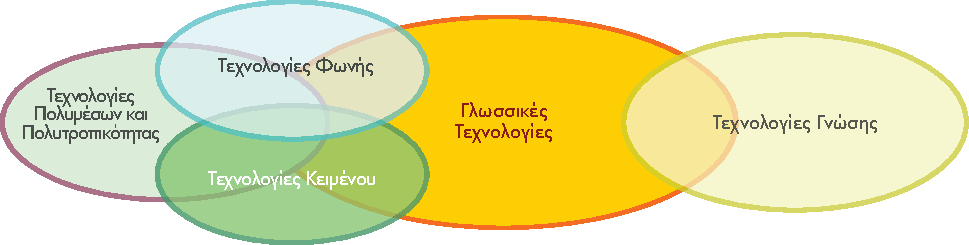
\includegraphics[width=\textwidth]{../_media/greek/language_technologies}
  \caption{Το τοπίο της Γλωσσικής Τεχνολογίας}
  \label{fig:ltincontext_de}
  \colorrule{grey3}{\textwidth}{1.5pt}
\end{figure*}

Στην επικοινωνία μας, συνδυάζουμε τη γλώσσα με άλλα μέσα επικοινωνίας και πληροφόρησης - για παράδειγμα ο προφορικός λόγος μπορεί να περιλαμβάνει χειρονομίες και εκφράσεις του προσώπου. Τα ψηφιακά κείμενα συνδυάζονται με εικόνες και ήχους. Οι ταινίες μπορεί να περιέχουν γλώσσα και σε προφορική και σε γραπτή μορφή. Με άλλα λόγια, οι τεχνολογίες προφορικού λόγου και κειμένου επικαλύπτονται και αλληλεπιδρούν με πολλές άλλες τεχνολογίες που διευκολύνουν την επεξεργασία της πολυτροπικής επικοινωνίας και των πολυμεσικών εγγράφων. 

Στη συνέχεια θα παρουσιαστούν τα βασικά πεδία εφαρμογών της ΓΤ, π.\,χ.~ο γλωσσικός έλεγχος, η αναζήτηση στο διαδίκτυο, η τεχνολογία φωνής και η μηχανική μετάφραση. Τα πεδία αυτά περιλαμβάνουν εφαρμογές όπως:

\begin{itemize}
\item διόρθωση ορθογραφικών λαθών
\item υποστήριξη συγγραφής κειμένου
\item εκμάθηση γλώσσας υποβοηθούμενη από υπολογιστή
\item ανάκτηση πληροφορίας
\item εξαγωγή πληροφορίας
\item αυτόματη περίληψη κειμένου
\item απάντηση ερωτημάτων
\item αναγνώριση φωνής 
\item σύνθεση φωνής
\end{itemize}

Η Γλωσσική τεχνολογία αποτελεί μια καθιερωμένη ερευνητική περιοχή με πλούσιο εισαγωγικό βιβλιογραφικό υλικό. Παρατίθενται ενδεικτικά οι ακόλουθες βιβλιογραφικές αναφορές: \cite{jurafsky-martin01,manning-schuetze1,lt-world1,lt-survey1}.

Πριν την ανάλυση των ανωτέρω πεδίων εφαρμογών θα περιγραφεί σύντομα η αρχιτεκτονική ενός τυπικού συστήματος ΓΤ. 

\subsection{Αρχιτεκτονικές Εφαρμογών}

Οι συνήθεις εφαρμογές λογισμικού για γλωσσική επεξεργασία συνήθως απαρτίζονται από διαφορετικά συστατικά μέρη που αντικατοπτρίζουν διάφορες πτυχές της γλώσσας. Το σχήμα~\ref{fig:textprocessingarch_de} εμφανίζει μια εξαιρετικά απλοποιημένη αρχιτεκτονική που απαντά σε ένα σύστημα επεξεργασίας κειμένου. Οι πρώτες τρεις λειτουργικές μονάδες χειρίζονται τη δομή και τη σημασία του εισαγόμενου κειμένου:

\begin{figure*}[b]
  \colorrule{grey3}{\textwidth}{1.5pt}
  \center
  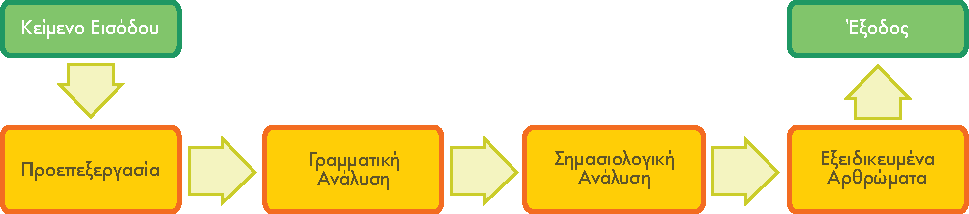
\includegraphics[width=\textwidth]{../_media/greek/text_processing_app_architecture}
  \caption{Τυπική Αρχιτεκτονική Εφαρμογής Επεξεργασίας Κειμένου}
  \label{fig:textprocessingarch_de}
  \colorrule{grey3}{\textwidth}{1.5pt}
\end{figure*}

\begin{enumerate}
\item Προ-επεξεργασία: καθαρισμός των δεδομένων, αφαίρεση μορφοποίησης, ανίχνευση της εισερχόμενης γλώσσας, των ορίων λέξης και πρότασης, κ.\,λπ.
\item Γραμματική ανάλυση: εύρεση του ρήματος και των αντικειμένων του, των προσδιορισμών και άλλων μερών του λόγου,  καθώς και της δομής της πρότασης.
\item Σημασιολογική ανάλυση: αποσαφήνιση (δηλ.~εντοπισμός της κατάλληλης σημασίας των λέξεων στο δεδομένο περικείμενο), επίλυση συναναφοράς και αναφορικών εκφράσεων (δηλ.~ποιες αντωνυμίες αναφέρονται σε ποια ουσιαστικά της πρότασης) και αναπαράσταση της σημασίας της πρότασης κατά τρόπο μηχανικά αναγνώσιμο.
\end{enumerate}

Στη συνέχεια, εξειδικευμένα αρθρώματα εκτελούν άλλες λειτουργίες, όπως η αυτόματη περίληψη κειμένου και η αναζήτηση σε βάσεις δεδομένων. Πρόκειται για μια απλοποιημένη περιγραφή της αρχιτεκτονικής που απεικονίζει την πολυπλοκότητα των εφαρμογών της ΓΤ. 

Μετά την εισαγωγή για τα βασικά πεδία εφαρμογών της ΓΤ θα ακολουθήσει μια σύντομη επισκόπηση της κατάστασης στην έρευνα και την εκπαίδευση της ΓΤ, καταλήγοντας με μια επισκόπηση παλαιών και τρεχουσών ερευνητικών δραστηριοτήτων. Στο τέλος αυτής της ενότητας, θα παρουσιάσουμε τις εκτιμήσεις εμπειρογνωμόνων αναφορικά με βασικά εργαλεία και πόρους ΓΤ ως προς αρκετές διαστάσεις, όπως η διαθεσιμότητα, η ωριμότητα και η ποιότητα. Η γενική εικόνα της κατάστασης της ΓΤ για την ελληνική γλώσσα συνοψίζεται στον πίνακα~\ref{fig:lrlttable_de} στη σελίδα~\pageref{fig:lrlttable_de}.

\subsection{Βασικά πεδία εφαρμογών} 

Η ενότητα αυτή εστιάζει στα πιο σημαντικά εργαλεία και πόρους ΓΤ και παρουσιάζει συνοπτικά τις δραστηριότητες της ΓΤ στην Ελλάδα. 

\subsubsection{Γλωσσικός έλεγχος}

Οποιοσδήποτε έχει χρησιμοποιήσει έναν κειμενογράφο όπως το Microsoft Word γνωρίζει ότι περιλαμβάνει έναν διορθωτή που επισημαίνει τα ορθογραφικά λάθη και προτείνει διορθώσεις. Οι πρώτοι ορθογραφικοί διορθωτές συνέκριναν τη λίστα των λέξεων του κειμένου με ένα λεξικό ορθογραφημένων λέξεων. Οι σύγχρονοι όμως διορθωτές είναι πολύ πιο εξελιγμένοι.  Με τη χρήση εξαρτώμενων από τη γλώσσα αλγόριθμων για την \textbf{γραμματική ανάλυση} εντοπίζουν λάθη που σχετίζονται με την μορφολογία (π.\,χ.~το σχηματισμό του πληθυντικού), όπως και συντακτικά λάθη, π.\,χ.~την έλλειψη ρήματος ή περιπτώσεις ασυμφωνίας ρήματος και υποκειμένου, π.\,χ.~"Μπορείτε να \textit{*προτείνεται} κάτι άλλο;" Εντούτοις, οι περισσότεροι διαθέσιμοι ορθογράφοι δεν θα βρουν κανένα λάθος στο ακόλουθο κείμενο \cite{zar1}:

\begin{quote}
  I have a spelling checker,\\
  It came with my PC.\\
  It plane lee marks four my revue\\
  Miss steaks aye can knot sea.
\end{quote}

Για το χειρισμό τέτοιου τύπου σφαλμάτων, η ανάλυση του περικειμένου είναι απαραίτητη σε πολλές περιπτώσεις, π.\,χ., για να κριθεί εάν μια λέξη είναι ρηματικός ή ονοματικός τύπος, όπως στο ακόλουθο παράδειγμα, όπου οι κλιτικοί τύποι  \textit{λύσης} (από το ουσιαστικό  \textit{λύση}) και  \textit{λύσεις} (από το ρήμα  \textit{λύνω}) ταυτίζονται φωνητικά αλλά διαφέρουν στην ορθογραφία και τη μορφοσυντακτική τους ταυτότητα:

\begin{itemize}
\item Μας παρουσίασε το σχέδιο της λύσης / \textit{*της λύσεις}.
\item Πρέπει να λύσεις / \textit{*λύσης} αυτό το πρόβλημα.
\end{itemize}

Αυτό απαιτεί είτε το σχηματισμό κανόνων \textbf{γραμματικής} ειδικών για κάθε γλώσσα, το οποίο συνεπάγεται μεγάλο βαθμό εξειδίκευσης και ανθρωποωρών ή τη χρήση ενός στατιστικού γλωσσικού μοντέλου. Αυτά τα μοντέλα υπολογίζουν την πιθανότητα μιας συγκεκριμένης λέξης να εμφανίζεται σε ένα συγκεκριμένο περιβάλλον (δηλαδή, τις προηγούμενες και τις επόμενες λέξεις). Για παράδειγμα, \textit{τις λύσεις} είναι μια πολύ πιο πιθανή ακολουθία λέξεων από το \textit{*τις λύσης}.
Ένα στατιστικό γλωσσικό μοντέλο μπορεί να παραχθεί αυτόματα χρησιμοποιώντας ένα μεγάλο όγκο (ορθών) γλωσσικών δεδομένων (π.\,χ.~ένα \textbf{σώμα κειμένων}). Μέχρι σήμερα, αυτές οι προσεγγίσεις έχουν κυρίως αναπτυχθεί και αξιολογηθεί σε αγγλικά γλωσσικά δεδομένα. Ωστόσο, αυτό δε σημαίνει ότι μπορούν να μεταφερθούν απαραίτητα απευθείας στα Ελληνικά, λόγω της ευέλικτης ακολουθίας των λέξεων και του πλούσιου κλιτικού συστήματος.

\boxtext{Η χρήση ορθογράφου δεν περιορίζεται\\ σε εργαλεία επεξεργασίας κειμένου, αλλά εφαρμόζεται επίσης σε συστήματα\\ υποβοήθησης συγγραφής κειμένου.}

Η χρήση Ορθογράφου δεν περιορίζεται σε εργαλεία επεξεργασίας κειμένου, αλλά εφαρμόζεται επίσης σε συστήματα  υποβοήθησης συγγραφής κειμένου, δηλαδή περιβάλλοντα λογισμικού στα οποία εγχειρίδια και λοιπά έγγραφα τεκμηρίωσης γράφονται σύμφωνα με συγκεκριμένα πρότυπα για σύνθετα προϊόντα στο χώρο της τεχνολογίας πληροφοριών, της υγείας, της μηχανολογίας κ.\,λπ.

\begin{figure*}[htb]
  \colorrule{grey3}{\textwidth}{1.5pt}
  %\vspace{-9mm}
  \center
  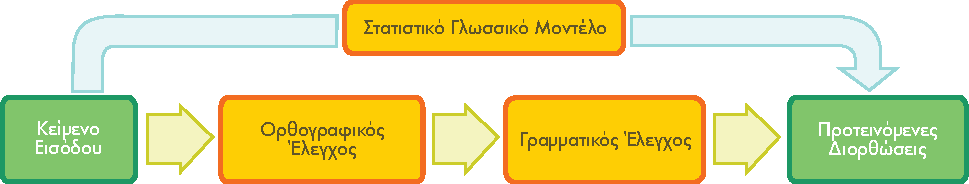
\includegraphics[width=\textwidth]{../_media/greek/language_checking}
  \caption{Γλωσσικός Έλεγχος (στατιστικός, βασισμένος σε κανόνες)}
  \label{fig:langcheckingaarch_de}
  \colorrule{grey3}{\textwidth}{1.5pt}
\end{figure*}

Φοβούμενοι τα παράπονα των πελατών για κακή χρήση και τις αγωγές αποζημιώσεων εξαιτίας ακατανόητων ή δυσνόητων οδηγιών, οι εταιρείες έχουν αρχίσει να εστιάζουν ολοένα και περισσότερο  στην ποιότητα της τεχνικής τεκμηρίωσης, στοχεύοντας παράλληλα στη διεθνή αγορά (μέσω της μετάφρασης ή της τοπικοποίησης). Οι εξελίξεις στην επεξεργασία της φυσικής γλώσσας οδηγούν στην ανάπτυξη λογισμικού υποβοήθησης συγγραφής κειμένου, το οποίο βοηθά τον συντάκτη τεχνικών εγγράφων να χρησιμοποιεί λεξιλόγιο και προτασιακές δομές  συμβατές με κανόνες και περιορισμούς της  (εταιρικής) ορολογίας. 

Λίγοι μόνο ελληνικοί οργανισμοί, εταιρείες και πάροχοι γλωσσικών υπηρεσιών προσφέρουν προϊόντα σε αυτόν τον τομέα. Το Ινστιτούτο Επεξεργασίας του Λόγου έχει αναπτύξει τη "Συμφωνία", μια εφαρμογή ελέγχου ορθογραφίας και γραμματικής συμφωνίας (π.\,χ.~άρθρου-ουσιασιτικού)  για την ελληνική γλώσσα. Δεν υπάρχει ακόμα κάποιος αξιόπιστος γραμματικός διορθωτής για τα Ελληνικά.

Πέρα από τους ορθογράφους και τη υποβοήθηση συγγραφής κειμένου, ο Γλωσσικός Έλεγχος είναι επίσης σημαντικός στον τομέα της εκμάθησης γλωσσών υποβοηθούμενης από υπολογιστή και επιπλέον εφαρμόζεται στην αυτόματη διόρθωση ερωτημάτων σε διαδικτυακές μηχανές αναζήτησης, π.\,χ.~στις προτάσεις ‘Μήπως εννοείτε…’ που προτείνει το Google.

\subsubsection{Αναζήτηση στο Διαδίκτυο}

Η αναζήτηση στο διαδίκτυο, σε εσωτερικά δίκτυα ή ψηφιακές βιβλιοθήκες είναι πιθανότατα η ευρύτερα χρησιμοποιούμενη αλλά παρόλ΄ αυτά η λιγότερο ανεπτυγμένη Γλωσσική Τεχνολογία σήμερα. Η μηχανή αναζήτησης Google, η οποία ξεκίνησε το 1998, χρησιμοποιείται σήμερα για περίπου το 80\% όλων των ερωτημάτων αναζήτησης παγκοσμίως \cite{spi1}. Από το 2007, το ρήμα \textit{γκουκγλάρω} ή \textit{γκουγκλίζω} έχει συμπεριληφθεί ως λήμμα σε ορισμένα ελληνικά λεξικά. Ούτε η διεπαφή αναζήτησης ούτε η παρουσίαση των ανακτημένων αποτελεσμάτων έχει αλλάξει σημαντικά σε σχέση με την πρώτη έκδοση. Στην τρέχουσα έκδοσή του, το Google προσφέρει ορθογραφική διόρθωση για ανορθόγραφες λέξεις κι επίσης, το 2009, ενσωμάτωσε δυνατότητες βασικής σημασιολογικής αναζήτησης στον αλγόριθμό του \cite{pc1}, ο οποίος μπορεί να βελτιώσει την ακρίβεια των αναζητήσεων αναλύοντας τη σημασία των όρων του ερωτήματος εντός περικειμένου. Η επιτυχία του Google δείχνει ότι διαθέτοντας πολλά δεδομένα και αποτελεσματικές τεχνικές για ευρετηρίαση αυτών των δεδομένων, μια στατιστική (κυρίως) προσέγγιση μπορεί να οδηγήσει σε ικανοποιητικά αποτελέσματα.

\begin{figure*}[htb]
  \colorrule{grey3}{\textwidth}{1.5pt}
  %\vspace{-9mm}
  \center
  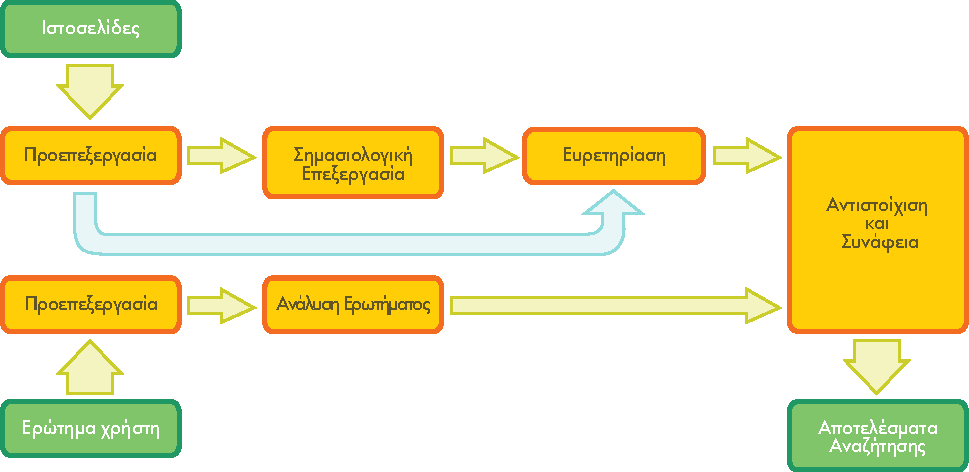
\includegraphics[width=\textwidth]{../_media/greek/web_search_architecture}
  %\vspace{-5mm}
  \caption{Αναζήτηση στον Ιστό}
  \label{fig:websearcharch_de}
  \colorrule{grey3}{\textwidth}{1.5pt}
\end{figure*}

Ωστόσο, για πιο προηγμένες αναζητήσεις   πληροφορίας  απαιτείται η ενσωμάτωση βαθύτερης γλωσσολογικής γνώσης για την ερμηνεία κειμένων. Πειράματα που χρησιμοποιούν \textbf{λεξιλογικούς πόρους}, όπως π.\,χ.~μηχανικά αναγνώσιμους γλωσσικούς θησαυρούς και οντολογικούς γλωσσικούς πόρους  όπως το WordNet, έχουν επιδείξει βελτιώσεις ως προς την ανεύρεση μιας σελίδας με βάση τα συνώνυμα των όρων αναζήτησης, π.\,χ.~\textit{ανανεώσιμες πηγές ενέργειας}, \textit{αιολική ενέργεια} ή ακόμα και όρους λιγότερο στενά συνδεδεμένους.

Η επόμενη γενιά μηχανών αναζήτησης θα πρέπει να συμπεριλάβει πολύ πιο προηγμένη Γλωσσική Τεχνολογία, κυρίως για αναζητήσεις που χρησιμοποιούν  ερώτηση ή άλλον τύπο πρότασης πέρα από μια λίστα λέξεων-κλειδιών. Για το ερώτημα \textit{Δώσε μου μια λίστα όλων των εταιρειών οι οποίες εξαγοράστηκαν από άλλες εταιρείες τα τελευταία πέντε χρόνια} το σύστημα ΓΤ πρέπει να αναλύσει την πρόταση συντακτικά και  \textbf{σημασιολογικά}, καθώς και να παρέχει ένα ευρετήριο που να επιτρέπει τη γρήγορη ανάκτηση των σχετικών εγγράφων. Μια ικανοποιητική απάντηση απαιτεί συντακτική ανάλυση για να αναγνωριστεί η γραμματική δομή της πρότασης και να καθοριστεί ότι ο χρήστης ψάχνει τις εταιρείες που εξαγοράστηκαν και όχι τις εταιρείες που εξαγόρασαν άλλες. Επίσης, για την έκφραση \textit{τα τελευταία πέντε χρόνια} το σύστημα χρειάζεται να προσδιορίσει το σχετικό χρονικό διάστημα. Και τέλος, το επεξεργασμένο ερώτημα πρέπει να αντιστοιχιστεί με έναν τεράστιο όγκο αδόμητων δεδομένων προκειμένου να βρεθεί το τμήμα ή τα τμήματα πληροφοριών που αναζητά ο χρήστης. Αυτό καλείται ‘ανάκτηση πληροφορίας’ και έχει να κάνει με την αναζήτηση και την κατάταξη σχετικών εγγράφων. Για την παραγωγή μιας λίστας εταιρειών χρειάζεται επίσης το σύστημα να αναγνωρίσει  μια συγκεκριμένη ακολουθία λέξεων σε ένα έγγραφο ως όνομα εταιρίας,  διαδικασία που ονομάζεται ‘αναγνώριση ονοματικών οντοτήτων’.

\boxtext{Η επόμενη γενιά μηχανών αναζήτησης\\ θα πρέπει να συμπεριλάβει πολύ πιο\\ εξεζητημένη Γλωσσική Τεχνολογία.}

Ακόμα πιο απαιτητική είναι η απόπειρα αντιστοίχισης ενός ερωτήματος που γίνεται σε μια γλώσσα με έγγραφα διαφορετικής γλώσσας. Η διαγλωσσική ανάκτηση πληροφορίας περιλαμβάνει την αυτόματη μετάφραση του ερωτήματος σε όλες τις πιθανές γλώσσες αναζήτησης, την εύρεση των αποτελεσμάτων και  την επακόλουθη μετάφρασής τους  στην αρχική γλώσσα του ερωτήματος.

Το αυξανόμενο ποσοστό δεδομένων που διατίθενται σε μη κειμενικές μορφές αυξάνει τη ζήτηση για υπηρεσίες που καθιστούν δυνατή την ανάκτηση πολυμεσικής πληροφορίας, δηλαδή την αναζήτηση πληροφορίας σε δεδομένα από εικόνες, ήχο και βίντεο. Στην περίπτωση των αρχείων ήχου και βίντεο, μια μονάδα αναγνώρισης φωνής πρέπει να μετατρέψει το προφορικό περιεχόμενο σε κείμενο (ή σε φωνητική αναπαράσταση), το οποίο στη συνέχεια αντιστοιχίζεται στο ερώτημα του χρήστη.

\subsubsection{Φωνητική Αλληλεπίδραση}

Η φωνητική αλληλεπίδραση είναι ένα από τα πολλά πεδία εφαρμογών που βασίζονται στην τεχνολογία φωνής, δηλαδή τις τεχνολογίες για την επεξεργασία του προφορικού λόγου. Οι τεχνολογίες φωνητικής αλληλεπίδρασης χρησιμοποιούνται για τη δημιουργία διεπαφών που επιτρέπουν στο χρήστη να αλληλεπιδρά χρησιμοποιώντας προφορικό λόγο αντί για οθόνη γραφικών, πληκτρολόγιο, ποντίκι, κ.\,λπ.~Σήμερα, τέτοιες φωνητικές διεπαφές χρήστη (VUI) χρησιμοποιούνται συνήθως για μερικώς ή πλήρως αυτοματοποιημένες τηλεφωνικές υπηρεσίες από εταιρείες προς τους πελάτες, τους εργαζομένους ή τους συνεταίρους τους. Επιχειρηματικοί κλάδοι που βασίζονται σε μεγάλο βαθμό σε VUI είναι οι τράπεζες, ο εφοδιασμός και διακίνηση προϊόντων (logistics), οι δημόσιες συγκοινωνίες και οι τηλεπικοινωνίες. Άλλες χρήσεις της τεχνολογίας φωνητικής αλληλεπίδρασης είναι οι διεπαφές συστημάτων πλοήγησης σε αυτοκίνητα και η χρήση της φωνής ως εναλλακτική της οθόνης γραφικών ή της οθόνης αφής στις έξυπνες τηλεφωνικές συσκευές (smartphones).

\begin{figure*}[htb]
  \colorrule{grey3}{\textwidth}{1.5pt}
  \center  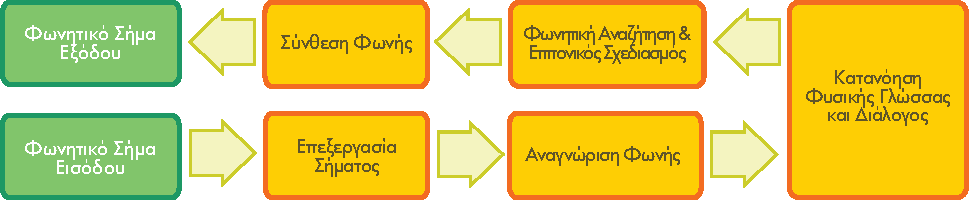
\includegraphics[width=\textwidth]{../_media/greek/simple_speech-based_dialogue_architecture}
  \center
  \caption{Διαλογικό Σύστημα βασισμένο σε Επεξεργασία Φωνής}
  \label{fig:dialoguearch_de}
  \colorrule{grey3}{\textwidth}{1.5pt}
\end{figure*}

Η φωνητική διάδραση περιλαμβάνει τις εξής επιμέρους τέσσερις διαφορετικές τεχνολογίες:

\begin{enumerate}
\item Η αυτόματη \textbf{αναγνώριση φωνής} (ASR) προσδιορίζει τις λέξεις που ειπώθηκαν δεδομένης μιας ακολουθίας ήχων που εκφέρει ο χρήστης.
\item Η τεχνολογία κατανόησης φυσικής γλώσσας αναλύει τη συντακτική δομή του εκφωνήματος του χρήστη και τις ερμηνεύει αναλόγως με το σκοπό του αντίστοιχου συστήματος.
\item τεχνολογία διαχείρισης διαλόγου καθορίζει τις ενέργειες που πρέπει να γίνουν αναλόγως με το εκφώνημα του χρήστη και τη λειτουργικότητα του εκάστοτε συστήματος.    
\item Η τεχνολογία \textbf{σύνθεσης φωνής} (TTS) μετατρέπει την απόκριση του συστήματος σε ήχους αντιληπτούς από το χρήστη.
\end{enumerate}

Μία από τις κύριες προκλήσεις των συστημάτων αναγνώρισης φωνής είναι η ακριβής αναγνώριση των λέξεων που αρθρώνει ο χρήστης. Αυτό απαιτεί είτε περιορισμό του εύρους των πιθανών εκφωνημάτων του χρήστη σε ένα ορισμένο σύνολο λέξεων-κλειδιών είτε τη χειρωνακτική δημιουργία γλωσσικών μοντέλων που καλύπτουν ένα ευρύ φάσμα εκφωνημάτων φυσικής γλώσσας. Μέσω της υιοθέτησης τεχνικών μηχανικής μάθησης τα γλωσσικά μοντέλα είναι δυνατόν να παραχθούν αυτόματα από  \textbf{σώματα κειμένων προφορικού λόγου}, δηλαδή από αρχεία ήχου και κειμενικές μεταγραφές αυτών. Ο περιορισμός των εκφωνημάτων συνήθως οδηγεί τους χρήστες σε μη ευέλικτη χρήση της φωνητικής διεπαφής, γεγονός που οδηγεί στην απόρριψή του. Όμως, η δημιουργία και η συντήρηση πλούσιων γλωσσικών μοντέλων αυξάνει το κόστος σημαντικά. Οι φωνητικές διεπαφές που χρησιμοποιούν γλωσσικά μοντέλα και επιτρέπουν ευελιξία στη διατύπωση της ερώτησης από τον  χρήστη  – με έναν χαιρετισμό  του τύπου \textit{Πώς μπορώ να σας βοηθήσω;} – τείνουν να αυτοματοποιηθούν και τυγχάνουν μεγαλύτερης αποδοχής από το χρήστη.

\boxtext{Οι τεχνολογίες φωνητικής διάδρασης είναι\\ η βάση δημιουργίας διεπαφών που\\ επιτρέπουν στο χρήστη να αλληλεπιδρά χρησιμοποιώντας προφορικό λόγο αντί\\ για οθόνη γραφικών, πληκτρολόγιο ή ποντίκι.}

Οι εταιρείες τείνουν να χρησιμοποιούν προηχογραφημένα εκφωνήματα επαγγελματιών ομιλητών για την παραγωγή του αποτελέσματος μιας VUI. Στην περίπτωση  στατικών εκφωνημάτων, στα οποία η διατύπωση δεν εξαρτάται από ιδιαίτερα περικείμενα χρήσης ή τα προσωπικά δεδομένα του συγκεκριμένου χρήστη, ο χρήστης έχει μια πολύ θετική εμπειρία. Ωστόσο, όσο πιο δυναμικό περιεχόμενο χρειάζεται να λάβει υπόψη της ένα εκφώνημα, τόσο περισσότερο μπορεί να επηρεαστεί αρνητικά η εμπειρία του χρήστη εξαιτίας του αφύσικου επιτονισμού που  οφείλεται στη σύνδεση μεμονωμένων ηχητικών αρχείων.Τα σημερινά συστήματα TTS βελτιώνονται, αν και επιδέχονται επιπλέον βελτιώσεων, όσον αφορά τη προσωδιακή φυσικότητα των εκφωνημάτων.

Οι εμπορικές διεπαφές χρήστη για τεχνολογίες φωνητικής αλληλεπίδρασης την τελευταία δεκαετία είναι σχετικά τυποποιημένες ως προς τα επιμέρους τεχνολογικά συστατικά. Παρατηρείται επίσης ισχυρή ενοποίηση της αγοράς στα πεδία της αναγνώρισης και σύνθεσης φωνής. Στις εθνικές αγορές των χωρών της G20 (οικονομικά εύρωστες χώρες με σημαντικό πληθυσμό) κυριαρχούν μόλις πέντε παίκτες παγκοσμίως, με την Nuance (ΗΠΑ) και την Loquendo (Ιταλία) να είναι οι επικρατέστερες εταιρείες  στην Ευρώπη. Το 2011 η Nuance ανακοίνωσε την απόκτηση της Loquendo, κίνηση η οποία αποτελεί ένα ακόμα βήμα προς την ενοποίηση της αγοράς

Στον χώρο της τεχνολογίας διαχείρισης διαλόγου και της σχετικής τεχνογνωσίας, οι αγορές κινούνται κυρίως σε εθνικό επίπεδο, με κυρίαρχους παίκτες μικρομεσαίες επιχειρήσεις. Αντί να βασίζονται αποκλειστικά σε μια επιχείρηση προϊόντων που εξαρτώνται από άδειες χρήσης λογισμικού, οι επιχειρήσεις αυτές προβάλλονται κυρίως ως πάροχοι ολοκληρωμένων υπηρεσιών που προσφέρουν τη δημιουργία VUI ως υπηρεσία ολοκλήρωσης συστήματος. Τέλος, στον κλάδο της φωνητικής αλληλεπίδρασης δεν υφίσταται ακόμα γνήσια αγορά για τις βασικές γλωσσικές τεχνολογίες συντακτικής και σημασιολογικής ανάλυσης.

Στην Ελλάδα, η ζήτηση για την πραγματική χρήση των VUI έχει αυξηθεί σημαντικά κατά την τελευταία πενταετία. Αυτή η τάση οφείλεται στην αυξανόμενη ζήτηση των τελικών πελατών για αυτοεξυπηρέτηση, στη σημαντική βελτιστοποίηση του κόστους των αυτοματοποιημένων τηλεφωνικών υπηρεσιών, καθώς και στη σημαντικά αυξημένη αποδοχή του προφορικού λόγου ως τρόπου επικοινωνίας  ανθρώπου-μηχανής.

Τέτοιες υπηρεσίες προσφέρονται από μικρομεσαίες επιχειρήσεις που προσαρμόζουν στην ελληνική γλώσσα ένα μείγμα από εισαγόμενες τεχνολογικές λύσεις, όπως αυτές που προαναφέρθηκαν, με εγχώριες τεχνολογικές λύσεις.

Στο άμεσο μέλλον θα υπάρξουν σημαντικές αλλαγές λόγω της διάδοσης των smartphones ως νέας πλατφόρμας διαχείρισης των πελατειακών σχέσεων – πέρα από το σταθερό τηλέφωνο, το διαδίκτυο και το ηλεκτρονικό ταχυδρομείο. Αυτή η τάση θα επηρεάσει επίσης την ανάπτυξη της τεχνολογίας φωνητικής αλληλεπίδρασης. Μακροπρόθεσμα, η ζήτηση για τις βασισμένες στο τηλέφωνο VUI θα μειωθεί, ενώ η χρήση της φωνής ως μιας φιλικής προς το χρήστη λειτουργικότητας εισόδου για smartphones θα αποκτήσει σημαντικό προβάδισμα. Αυτή η τάση υποστηρίζεται από την παρατηρούμενη βελτίωση της ακρίβειας στην αναγνώριση φωνής ανεξαρτήτως ομιλητή στις υπηρεσίες υπαγόρευσης που είναι ήδη διαθέσιμες ως υπηρεσίες σε χρήστες smartphone.

\subsubsection{Μηχανική Μετάφραση}

Την ιδέα της χρήσης ψηφιακών υπολογιστών για τη μετάφραση φυσικών γλωσσών χρονολογείται από το 1946 . Σημαντική χρηματοδότηση δόθηκε για την έρευνα σε αυτόν τον τομέα στη δεκαετία του 1950 και πάλι στη δεκαετία του 1980. Εντούτοις, η \textbf{Μηχανική Μετάφραση} (ΜΜ) εξακολουθεί να αδυνατεί να ικανοποιήσει τις υψηλές προσδοκίες πλήρους αυτόματης μετάφρασης που δημιούργησε στα πρώτα της χρόνια.

\boxtext{Η απλούστερη προσέγγιση στη ΜΜ είναι η αυτόματη αντικατάσταση των λέξεων μιας φυσικής γλώσσας με λέξεις μιας άλλης γλώσσας.}

Η απλούστερη προσέγγιση στη ΜΜ είναι η αυτόματη αντικατάσταση των λέξεων ενός κειμένου γραμμένου σε μια φυσική γλώσσα με λέξεις μιας άλλης γλώσσας. Αυτό μπορεί να είναι χρήσιμο σε θεματικούς τομείς με πολύ περιορισμένη και τυποποιημένη γλώσσα, όπως π.\,χ.~τα μετεωρολογικά δελτία. Ωστόσο, η καλή μετάφραση λιγότερο τυποποιημένων και μεγαλύτερων κειμένων (φράσεων, προτάσεων ή ακόμα και ολόκληρων αποσπασμάτων) απαιτεί την αντιστοίχιση με τα πιο κοντινά τους ισοδύναμα στη γλώσσα στόχο. Η μεγαλύτερη δυσκολία εν προκειμένω έγκειται στο γεγονός ότι η ανθρώπινη γλώσσα είναι αμφίσημη, πράγμα το οποίο γεννά προκλήσεις σε πολλαπλά επίπεδα, π.\,χ., την αποσαφήνιση της σημασίας των λέξεων σε λεξιλογικό επίπεδο (η λέξη \textit{τζάγκουαρ} μπορεί να αναφέρεται σε αυτοκίνητο ή ζώο) ή την προσάρτηση εμπρόθετων φράσεων σε συντακτικό επίπεδο όπως παρακάτω:

\begin{itemize}
\item Ο αστυνομικός παρακολουθεί τη γυναίκα με τα κιάλια.
\item Ο αστυνομικός παρακολουθεί τη γυναίκα με το περίστροφο.
\end{itemize}

Ένας τρόπος ανάπτυξης συστημάτων ΜΜ βασίζεται στη χρήση  γλωσσολογικών κανόνων. Για μεταφράσεις ανάμεσα σε συγγενικές γλώσσες, μια λέξη προς λέξη υποκατάσταση μπορεί να είναι εφικτή σε περιπτώσεις όπως το προηγούμενο παράδειγμα. Όμως, τα συστήματα που βασίζονται σε κανόνες (ή σε γλωσσολογική γνώση) συνήθως αναλύουν το εισερχόμενο κείμενο και δημιουργούν μια ενδιάμεση, συμβολική αναπαράσταση, από την οποία παράγεται το κείμενο στη γλώσσα στόχο. Η επιτυχία αυτών των μεθόδων εξαρτάται σε μεγάλο βαθμό από τη διαθεσιμότητα εκτεταμένων λεξικών με μορφολογική, συντακτική και σημασιολογική πληροφορία και μεγάλα σύνολα γραμματικών κανόνων καταρτισμένων από εξειδικευμένους γλωσσολόγους. Αυτή όμως είναι μια πολύ μακροχρόνια και, επομένως, δαπανηρή διαδικασία.

\begin{figure*}[htb]
  \colorrule{grey3}{\textwidth}{1.5pt}
  \center
  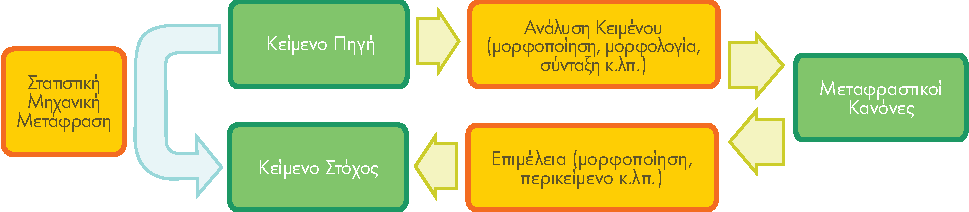
\includegraphics[width=\textwidth]{../_media/greek/machine_translation}
  \caption{Μηχανική Μετάφραση (στατιστική, βασισμένη σε κανόνες)}
  \label{fig:mtarch_de}
  \colorrule{grey3}{\textwidth}{1.5pt}
\end{figure*}

Στα τέλη της δεκαετίας του 1980, καθώς η υπολογιστική ισχύς αυξήθηκε και έγινε λιγότερο δαπανηρή, παρατηρήθηκε  μεγαλύτερο ενδιαφέρον για στατιστικά μοντέλα ΜΜ. Τα στατιστικά μοντέλα προέρχονται από την ανάλυση δίγλωσσων \textbf{σωμάτων παράλληλων κειμένων}, όπως είναι για παράδειγμα το Europarl, το οποίο περιλαμβάνει τα πρακτικά του Ευρωπαϊκού Κοινοβουλίου σε 11 ευρωπαϊκές γλώσσες. Εάν υπάρχουν αρκετά δεδομένα, η στατιστική MΜ αποδίδει αρκετά καλά ως προς την παραγωγή κατά προσέγγιση νοήματος ενός ξενόγλωσσου κειμένου μέσω της επεξεργασίας παράλληλων δεδομένων και της ανεύρεσης πιθανών αντιστοιχίσεων λέξεων. Εντούτοις, σε αντίθεση με τα συστήματα που βασίζονται σε γλωσσολογική γνώση, η στατιστική (ή βασισμένη σε δεδομένα) MΜ συχνά παράγει γραμματικά εσφαλμένα αποτελέσματα. Η βασισμένη σε δεδομένα ΜΜ υπερτερεί στο ότι απαιτεί μικρότερη ανθρώπινη προσπάθεια, και στο ότι έχει τη δυνατότητα να χειρίζεται ιδιαιτερότητες της γλώσσας (π.\,χ.~ιδιωματισμούς) που τα συστήματα που βασίζονται σε γλωσσολογική γνώση πιθανόν να αγνοήσουν.

Καθώς τα πλεονεκτήματα και τα μειονεκτήματα της βασισμένης στη γλωσσολογική γνώση και στα δεδομένα MΜ αλληλοσυμπληρώνονται, οι ερευνητές σήμερα προσανατολίζονται σε υβριδικές προσεγγίσεις που συνδυάζουν και τις δύο μεθοδολογίες. Μία από αυτές συνδυάζει συστήματα βασισμένα στη γλωσσολογική γνώση και συστήματα βασισμένα στα δεδομένα μαζί με μια μονάδα επιλογής, η οποία αποφασίζει ποιο είναι το καλύτερο αποτέλεσμα για κάθε πρόταση. Εντούτοις, τα αποτελέσματα για προτάσεις μεγαλύτερες των 12 λέξεων συνήθως δεν είναι ικανοποιητικά. Επομένως, μια καλύτερη λύση είναι να συνδυαστούν τα καλύτερα τμήματα κάθε πρότασης από πολλαπλά αποτελέσματα, κάτι που είναι αρκετά περίπλοκο καθώς οι αντιστοιχίες των πολλαπλών αυτών εναλλακτικών δεν είναι πάντοτε προφανείς και χρειάζονται στοίχιση. Η χρήση της ΜΜ είναι δυνατόν να αυξήσει σημαντικά την παραγωγικότητα εάν προσαρμοστεί κατάλληλα στην ορολογία και ενταχθεί στη ροή εργασιών. Οι γλωσσικές πύλες παρέχουν πρόσβαση σε λεξικά και εξειδικευμένη ορολογία, καθώς και σε υποστήριξη μεταφραστικών μνημών και ΜΜ. 

Η ποιότητα των συστημάτων MΜ θεωρείται ότι έχει ακόμη τεράστιες δυνατότητες βελτίωσης. Στις προκλήσεις συγκαταλέγονται η δυνατότητα προσαρμογής των γλωσσικών πόρων σε ένα δεδομένο θεματικό πεδίο ή στον τομέα του χρήστη και η ενσωμάτωση σε υπάρχουσες ροές εργασιών με βάσεις δεδομένων και μεταφραστικές μνήμες. Επίσης, τα περισσότερα από τα τρέχοντα συστήματα είναι επικεντρωμένα στα αγγλικά και υποστηρίζουν μόνο λίγες γλώσσες σε συνδυασμό με τα ελληνικά, γεγονός  που δημιουργεί προβλήματα σε ολόκληρη τη ροή μεταφραστικών εργασιών και π.\,χ.~αναγκάζει τους χρήστες της MΜ να μαθαίνουν διαφορετικά εργαλεία για διαφορετικά συστήματα.

\boxtext{Η μηχανική μετάφραση για την ελληνική γλώσσα παρουσιάζει ιδιαίτερες προκλήσεις.} 

Η μηχανική μετάφραση για τα ελληνικά παρουσιάζει ιδιαίτερες προκλήσεις. Η ελεύθερη σειρά των όρων της πρότασης  θέτει προβλήματα στην διαδικασία της ανάλυσης, και το πλούσιο κλιτικό σύστημα αποτελεί πρόκληση για τη διαδικασία παραγωγής λέξεων στο σωστό γένος και πτώση. Σε εθνικό επίπεδο, υπάρχουν μικρές εταιρείες-τεχνοβλαστοί που προσπαθούν να κατακτήσουν μια θέση στην αγορά ενσωματώνοντας λύσεις Μεταφραστικών Μνημών και Στατιστικής Μηχανικής Μετάφρασης, υποστηρίζοντας κυρίως τα ελληνικά σε συνδυασμό με τα αγγλικά, τα γαλλικά και τα γερμανικά.

Δράσεις αξιολόγησης επιτρέπουν τη σύγκριση των συστημάτων MΜ ως προς την ποιότητά τους, τις διαφορετικές προσεγγίσεις και την απόδοσή τους για τα διαφορετικά γλωσσικά ζεύγη. Στον ακόλουθο πίνακα, ο οποίος καταρτίστηκε στο πλαίσιο του ευρωπαϊκού έργου Euromatrix+, περιγράφονται οι κατά ζεύγη επιδόσεις για 22 από τις 23 επίσημες γλώσσες της ΕΕ (εκτός της ιρλανδικής). Η κατάταξη των αποτελεσμάτων ακολουθεί τη βαθμολογία BLEU, η οποία δίνει υψηλότερα σκορ για τις καλύτερες μεταφράσεις \cite{bleu1}. Με αυτή τη μέθοδο, η βαθμολογία ενός ανθρώπου μεταφραστή θα ανερχόταν στους 80 βαθμούς.

Τα καλύτερα αποτελέσματα (με πράσινο και μπλε) επιτεύχθηκαν από γλώσσες που χαρακτηρίζονται από σημαντική ερευνητική δραστηριότητα μέσα από συντονισμένα προγράμματα καθώς και από την ύπαρξη πολλών παράλληλων σωμάτων κειμένων (π.\,χ.~αγγλικά, γαλλικά, ολλανδικά, ισπανικά, γερμανικά). Τα χειρότερα αποτελέσματα (με κόκκινο) αφορούν σε γλώσσες με περιορισμένη ερευνητική δραστηριότητα ή σε γλώσσες που είναι δομικά πολύ διαφορετικές από άλλες (π.\,χ.~ουγγρικά, μαλτέζικα, φινλανδικά).

\begin{figure*}[tb]
  \centering
  \setlength{\tabcolsep}{0.17em}
  \small
  \begin{tabular}{>{\columncolor{corange1}}cccccccccccccccccccccccc}
    & \multicolumn{22}{>{\columncolor{corange1}}c}{Γλώσσα στόχος -- \textcolor{grey1}{Target language}}\\\addlinespace[{-.009cm}]
    \rowcolor{corange1}  & EN & BG & DE & CS & DA & EL & ES & ET & FI & FR & HU & IT & LT & LV & MT & NL & PL & PT & RO & SK & SL & SV\\
    EN & -- & \textcolor{blue}{40.5} & \textcolor{blue}{46.8} & \textcolor{green2}{52.6} & \textcolor{green2}{50.0} & \textcolor{blue}{41.0} & \textcolor{green2}{55.2} & \textcolor{purple}{34.8} & \textcolor{purple}{38.6} & \textcolor{green2}{50.1} & \textcolor{purple}{37.2} & \textcolor{green2}{50.4} & \textcolor{purple}{39.6} & \textcolor{blue}{43.4} & \textcolor{purple}{39.8} & \textcolor{green2}{52.3} & \textcolor{blue}{49.2} & \textcolor{green2}{55.0} & \textcolor{blue}{49.0} & \textcolor{blue}{44.7} & \textcolor{green2}{50.7} & \textcolor{green2}{52.0}\\
    BG & \textcolor{green}{61.3} & -- & \textcolor{purple}{38.7} & \textcolor{purple}{39.4} & \textcolor{purple}{39.6} & \textcolor{purple}{34.5} & \textcolor{blue}{46.9} & \textcolor{red3}{25.5} & \textcolor{red3}{26.7} & \textcolor{blue}{42.4} & \textcolor{red3}{22.0} & \textcolor{blue}{43.5} & \textcolor{red3}{29.3} & \textcolor{red3}{29.1} & \textcolor{red3}{25.9} & \textcolor{blue}{44.9} & \textcolor{purple}{35.1} & \textcolor{blue}{45.9} & \textcolor{purple}{36.8} & \textcolor{purple}{34.1} & \textcolor{purple}{34.1} & \textcolor{purple}{39.9}\\
    DE & \textcolor{green2}{53.6} & \textcolor{red3}{26.3} & -- & \textcolor{purple}{35.4} & \textcolor{blue}{43.1} & \textcolor{purple}{32.8} & \textcolor{blue}{47.1} & \textcolor{red3}{26.7} & \textcolor{red3}{29.5} & \textcolor{purple}{39.4} & \textcolor{red3}{27.6} & \textcolor{blue}{42.7} & \textcolor{red3}{27.6} & \textcolor{purple}{30.3} & \textcolor{red2}{19.8} & \textcolor{green2}{50.2} & \textcolor{purple}{30.2} & \textcolor{blue}{44.1} & \textcolor{purple}{30.7} & \textcolor{red3}{29.4} & \textcolor{purple}{31.4} & \textcolor{blue}{41.2}\\
    CS & \textcolor{green2}{58.4} & \textcolor{purple}{32.0} & \textcolor{blue}{42.6} & -- & \textcolor{blue}{43.6} & \textcolor{purple}{34.6} & \textcolor{blue}{48.9} & \textcolor{purple}{30.7} & \textcolor{purple}{30.5} & \textcolor{blue}{41.6} & \textcolor{red3}{27.4} & \textcolor{blue}{44.3} & \textcolor{purple}{34.5} & \textcolor{purple}{35.8} & \textcolor{red3}{26.3} & \textcolor{blue}{46.5} & \textcolor{purple}{39.2} & \textcolor{blue}{45.7} & \textcolor{purple}{36.5} & \textcolor{blue}{43.6} & \textcolor{blue}{41.3} & \textcolor{blue}{42.9}\\
    DA & \textcolor{green2}{57.6} & \textcolor{red3}{28.7} & \textcolor{blue}{44.1} & \textcolor{purple}{35.7} & -- & \textcolor{purple}{34.3} & \textcolor{blue}{47.5} & \textcolor{red3}{27.8} & \textcolor{purple}{31.6} & \textcolor{blue}{41.3} & \textcolor{red3}{24.2} & \textcolor{blue}{43.8} & \textcolor{red3}{29.7} & \textcolor{purple}{32.9} & \textcolor{red3}{21.1} & \textcolor{blue}{48.5} & \textcolor{purple}{34.3} & \textcolor{blue}{45.4} & \textcolor{purple}{33.9} & \textcolor{purple}{33.0} & \textcolor{purple}{36.2} & \textcolor{blue}{47.2}\\
    EL & \textcolor{green2}{59.5} & \textcolor{purple}{32.4} & \textcolor{blue}{43.1} & \textcolor{purple}{37.7} & \textcolor{blue}{44.5} & -- & \textcolor{green2}{54.0} & \textcolor{red3}{26.5} & \textcolor{red3}{29.0} & \textcolor{blue}{48.3} & \textcolor{red3}{23.7} & \textcolor{blue}{49.6} & \textcolor{red3}{29.0} & \textcolor{purple}{32.6} & \textcolor{red3}{23.8} & \textcolor{blue}{48.9} & \textcolor{purple}{34.2} & \textcolor{green2}{52.5} & \textcolor{purple}{37.2} & \textcolor{purple}{33.1} & \textcolor{purple}{36.3} & \textcolor{blue}{43.3}\\
    ES & \textcolor{green}{60.0} & \textcolor{purple}{31.1} & \textcolor{blue}{42.7} & \textcolor{purple}{37.5} & \textcolor{blue}{44.4} & \textcolor{purple}{39.4} & -- & \textcolor{red3}{25.4} & \textcolor{red3}{28.5} & \textcolor{green2}{51.3} & \textcolor{red3}{24.0} & \textcolor{green2}{51.7} & \textcolor{red3}{26.8} & \textcolor{purple}{30.5} & \textcolor{red3}{24.6} & \textcolor{blue}{48.8} & \textcolor{purple}{33.9} & \textcolor{green2}{57.3} & \textcolor{purple}{38.1} & \textcolor{purple}{31.7} & \textcolor{purple}{33.9} & \textcolor{blue}{43.7}\\
    ET & \textcolor{green2}{52.0} & \textcolor{red3}{24.6} & \textcolor{purple}{37.3} & \textcolor{purple}{35.2} & \textcolor{purple}{37.8} & \textcolor{red3}{28.2} & \textcolor{blue}{40.4} & -- & \textcolor{purple}{37.7} & \textcolor{purple}{33.4} & \textcolor{purple}{30.9} & \textcolor{purple}{37.0} & \textcolor{purple}{35.0} & \textcolor{purple}{36.9} & \textcolor{red3}{20.5} & \textcolor{blue}{41.3} & \textcolor{purple}{32.0} & \textcolor{purple}{37.8} & \textcolor{red3}{28.0} & \textcolor{purple}{30.6} & \textcolor{purple}{32.9} & \textcolor{purple}{37.3}\\
    FI & \textcolor{blue}{49.3} & \textcolor{red3}{23.2} & \textcolor{purple}{36.0} & \textcolor{purple}{32.0} & \textcolor{purple}{37.9} & \textcolor{red3}{27.2} & \textcolor{purple}{39.7} & \textcolor{purple}{34.9} & -- & \textcolor{red3}{29.5} & \textcolor{red3}{27.2} & \textcolor{purple}{36.6} & \textcolor{purple}{30.5} & \textcolor{purple}{32.5} & \textcolor{red2}{19.4} & \textcolor{blue}{40.6} & \textcolor{red3}{28.8} & \textcolor{purple}{37.5} & \textcolor{red3}{26.5} & \textcolor{red3}{27.3} & \textcolor{red3}{28.2} & \textcolor{purple}{37.6}\\
    FR & \textcolor{green}{64.0} & \textcolor{purple}{34.5} & \textcolor{blue}{45.1} & \textcolor{purple}{39.5} & \textcolor{blue}{47.4} & \textcolor{blue}{42.8} & \textcolor{green}{60.9} & \textcolor{red3}{26.7} & \textcolor{purple}{30.0} & -- & \textcolor{red3}{25.5} & \textcolor{green2}{56.1} & \textcolor{red3}{28.3} & \textcolor{purple}{31.9} & \textcolor{red3}{25.3} & \textcolor{green2}{51.6} & \textcolor{purple}{35.7} & \textcolor{green}{61.0} & \textcolor{blue}{43.8} & \textcolor{purple}{33.1} & \textcolor{purple}{35.6} & \textcolor{blue}{45.8}\\
    HU & \textcolor{blue}{48.0} & \textcolor{red3}{24.7} & \textcolor{purple}{34.3} & \textcolor{purple}{30.0} & \textcolor{purple}{33.0} & \textcolor{red3}{25.5} & \textcolor{purple}{34.1} & \textcolor{red3}{29.6} & \textcolor{red3}{29.4} & \textcolor{purple}{30.7} & -- & \textcolor{purple}{33.5} & \textcolor{red3}{29.6} & \textcolor{purple}{31.9} & \textcolor{red2}{18.1} & \textcolor{purple}{36.1} & \textcolor{red3}{29.8} & \textcolor{purple}{34.2} & \textcolor{red3}{25.7} & \textcolor{red3}{25.6} & \textcolor{red3}{28.2} & \textcolor{purple}{30.5}\\
    IT & \textcolor{green}{61.0} & \textcolor{purple}{32.1} & \textcolor{blue}{44.3} & \textcolor{purple}{38.9} & \textcolor{blue}{45.8} & \textcolor{blue}{40.6} & \textcolor{red3}{26.9} & \textcolor{red3}{25.0} & \textcolor{red3}{29.7} & \textcolor{green2}{52.7} & \textcolor{red3}{24.2} & -- & \textcolor{red3}{29.4} & \textcolor{purple}{32.6} & \textcolor{red3}{24.6} & \textcolor{green2}{50.5} & \textcolor{purple}{35.2} & \textcolor{green2}{56.5} & \textcolor{purple}{39.3} & \textcolor{purple}{32.5} & \textcolor{purple}{34.7} & \textcolor{blue}{44.3}\\
    LT & \textcolor{green2}{51.8} & \textcolor{red3}{27.6} & \textcolor{purple}{33.9} & \textcolor{purple}{37.0} & \textcolor{purple}{36.8} & \textcolor{red3}{26.5} & \textcolor{red3}{21.1} & \textcolor{purple}{34.2} & \textcolor{purple}{32.0} & \textcolor{purple}{34.4} & \textcolor{red3}{28.5} & \textcolor{purple}{36.8} & -- & \textcolor{blue}{40.1} & \textcolor{red3}{22.2} & \textcolor{purple}{38.1} & \textcolor{purple}{31.6} & \textcolor{purple}{31.6} & \textcolor{red3}{29.3} & \textcolor{purple}{31.8} & \textcolor{purple}{35.3} & \textcolor{purple}{35.3}\\
    LV & \textcolor{green2}{54.0} & \textcolor{red3}{29.1} & \textcolor{purple}{35.0} & \textcolor{purple}{37.8} & \textcolor{purple}{38.5} & \textcolor{red3}{29.7} & \textcolor{red2}{8.0} & \textcolor{purple}{34.2} & \textcolor{purple}{32.4} & \textcolor{purple}{35.6} & \textcolor{red3}{29.3} & \textcolor{purple}{38.9} & \textcolor{purple}{38.4} & -- & \textcolor{red3}{23.3} & \textcolor{blue}{41.5} & \textcolor{purple}{34.4} & \textcolor{purple}{39.6} & \textcolor{purple}{31.0} & \textcolor{purple}{33.3} & \textcolor{purple}{37.1} & \textcolor{purple}{38.0}\\
    MT & \textcolor{green}{72.1} & \textcolor{purple}{32.2} & \textcolor{purple}{37.2} & \textcolor{purple}{37.9} & \textcolor{purple}{38.9} & \textcolor{purple}{33.7} & \textcolor{blue}{48.7} & \textcolor{red3}{26.9} & \textcolor{red3}{25.8} & \textcolor{blue}{42.4} & \textcolor{red3}{22.4} & \textcolor{blue}{43.7} & \textcolor{purple}{30.2} & \textcolor{purple}{33.2} & -- & \textcolor{blue}{44.0} & \textcolor{purple}{37.1} & \textcolor{blue}{45.9} & \textcolor{purple}{38.9} & \textcolor{purple}{35.8} & \textcolor{blue}{40.0} & \textcolor{blue}{41.6}\\
    NL & \textcolor{green2}{56.9} & \textcolor{red3}{29.3} & \textcolor{blue}{46.9} & \textcolor{purple}{37.0} & \textcolor{blue}{45.4} & \textcolor{purple}{35.3} & \textcolor{blue}{49.7} & \textcolor{red3}{27.5} & \textcolor{red3}{29.8} & \textcolor{blue}{43.4} & \textcolor{red3}{25.3} & \textcolor{blue}{44.5} & \textcolor{red3}{28.6} & \textcolor{purple}{31.7} & \textcolor{red3}{22.0} & -- & \textcolor{purple}{32.0} & \textcolor{blue}{47.7} & \textcolor{purple}{33.0} & \textcolor{purple}{30.1} & \textcolor{purple}{34.6} & \textcolor{blue}{43.6}\\
    PL & \textcolor{green}{60.8} & \textcolor{purple}{31.5} & \textcolor{blue}{40.2} & \textcolor{blue}{44.2} & \textcolor{blue}{42.1} & \textcolor{purple}{34.2} & \textcolor{blue}{46.2} & \textcolor{red3}{29.2} & \textcolor{red3}{29.0} & \textcolor{blue}{40.0} & \textcolor{red3}{24.5} & \textcolor{blue}{43.2} & \textcolor{purple}{33.2} & \textcolor{purple}{35.6} & \textcolor{red3}{27.9} & \textcolor{blue}{44.8} & -- & \textcolor{blue}{44.1} & \textcolor{purple}{38.2} & \textcolor{purple}{38.2} & \textcolor{purple}{39.8} & \textcolor{blue}{42.1}\\
    PT & \textcolor{green}{60.7} & \textcolor{purple}{31.4} & \textcolor{blue}{42.9} & \textcolor{purple}{38.4} & \textcolor{blue}{42.8} & \textcolor{blue}{40.2} & \textcolor{green}{60.7} & \textcolor{red3}{26.4} & \textcolor{red3}{29.2} & \textcolor{green2}{53.2} & \textcolor{red3}{23.8} & \textcolor{green2}{52.8} & \textcolor{red3}{28.0} & \textcolor{purple}{31.5} & \textcolor{red3}{24.8} & \textcolor{blue}{49.3} & \textcolor{purple}{34.5} & -- & \textcolor{purple}{39.4} & \textcolor{purple}{32.1} & \textcolor{purple}{34.4} & \textcolor{blue}{43.9}\\
    RO & \textcolor{green}{60.8} & \textcolor{purple}{33.1} & \textcolor{purple}{38.5} & \textcolor{purple}{37.8} & \textcolor{blue}{40.3} & \textcolor{purple}{35.6} & \textcolor{green2}{50.4} & \textcolor{red3}{24.6} & \textcolor{red3}{26.2} & \textcolor{blue}{46.5} & \textcolor{red3}{25.0} & \textcolor{blue}{44.8} & \textcolor{red3}{28.4} & \textcolor{red3}{29.9} & \textcolor{red3}{28.7} & \textcolor{blue}{43.0} & \textcolor{purple}{35.8} & \textcolor{blue}{48.5} & -- & \textcolor{purple}{31.5} & \textcolor{purple}{35.1} & \textcolor{purple}{39.4}\\
    SK & \textcolor{green}{60.8} & \textcolor{purple}{32.6} & \textcolor{purple}{39.4} & \textcolor{blue}{48.1} & \textcolor{blue}{41.0} & \textcolor{purple}{33.3} & \textcolor{blue}{46.2} & \textcolor{red3}{29.8} & \textcolor{red3}{28.4} & \textcolor{purple}{39.4} & \textcolor{red3}{27.4} & \textcolor{blue}{41.8} & \textcolor{purple}{33.8} & \textcolor{purple}{36.7} & \textcolor{red3}{28.5} & \textcolor{blue}{44.4} & \textcolor{purple}{39.0} & \textcolor{blue}{43.3} & \textcolor{purple}{35.3} & -- & \textcolor{blue}{42.6} & \textcolor{blue}{41.8}\\
    SL & \textcolor{green}{61.0} & \textcolor{purple}{33.1} & \textcolor{purple}{37.9} & \textcolor{blue}{43.5} & \textcolor{blue}{42.6} & \textcolor{purple}{34.0} & \textcolor{blue}{47.0} & \textcolor{purple}{31.1} & \textcolor{red3}{28.8} & \textcolor{purple}{38.2} & \textcolor{red3}{25.7} & \textcolor{blue}{42.3} & \textcolor{purple}{34.6} & \textcolor{purple}{37.3} & \textcolor{purple}{30.0} & \textcolor{blue}{45.9} & \textcolor{purple}{38.2} & \textcolor{blue}{44.1} & \textcolor{purple}{35.8} & \textcolor{purple}{38.9} & -- & \textcolor{blue}{42.7}\\
    SV & \textcolor{green2}{58.5} & \textcolor{red3}{26.9} & \textcolor{blue}{41.0} & \textcolor{purple}{35.6} & \textcolor{blue}{46.6} & \textcolor{purple}{33.3} & \textcolor{blue}{46.6} & \textcolor{red3}{27.4} & \textcolor{purple}{30.9} & \textcolor{purple}{38.9} & \textcolor{red3}{22.7} & \textcolor{blue}{42.0} & \textcolor{red3}{28.2} & \textcolor{purple}{31.0} & \textcolor{red3}{23.7} & \textcolor{blue}{45.6} & \textcolor{purple}{32.2} & \textcolor{blue}{44.2} & \textcolor{purple}{32.7} & \textcolor{purple}{31.3} & \textcolor{purple}{33.5} & --\\
    \end{tabular}
  \caption{Μηχανική Μετάφραση μεταξύ 22 ευρωπαϊκών γλωσσών -- \textcolor{grey1}{Machine translation between 22 EU-languages \cite{euro1}}}
  \label{fig:euromatrix_de}
\end{figure*}

\subsection{Άλλα πεδία εφαρμογών}

Η δημιουργία εφαρμογών Γλωσσικής Τεχνολογίας περιλαμβάνει ευρύ φάσμα επιμέρους εργασιών οι οποίες δεν είναι πάντα αντιληπτές  από τον χρήστη,  αλλά προσφέρουν σημαντικές λειτουργικότητες 'στο παρασκήνιο' του εκάστοτε συστήματος. Για το λόγο αυτό συνιστούν σημαντικά ερευνητικά ζητήματα που έχουν εξελιχθεί σε διακριτούς κλάδους της Υπολογιστικής Γλωσσολογίας. 

\boxtext{Οι εφαρμογές γλωσσικής τεχνολογίας\\ συχνά παρέχουν σημαντικές\\ λειτουργικότητες ενσωματωμένες σε\\ μεγαλύτερα συστήματα λογισμικού.}

Για παράδειγμα, τα συστήματα ερωταποκρίσεων έχουν εξελιχθεί σε ένα δυναμικό πεδίο έρευνας, για το οποίο έχουν αναπτυχθεί επισημειωμένα σχολιασμένα σώματα κειμένων, ενώ έχουν διενεργηθεί και σχετικοί επιστημονικοί διαγωνισμοί. Η λογική πίσω από τα συστήματα ερωταποκρίσεων βρίσκεται πέρα από την αναζήτηση με λέξεις κλειδιά (στην οποία η μηχανή αναζήτησης επιστρέφει μια συλλογή πιθανά σχετιζόμενων εγγράφων) δεδομένου ότι δίνει στον χρήστη τη δυνατότητα να απευθύνει μια συγκεκριμένη ερώτηση για την οποία το σύστημα παρέχει μια μοναδική απάντηση. Για παράδειγμα:

\begin{itemize}
\item[] \textit{Ερώτηση: Σε ποια ηλικία πάτησε ο Neil Armstrong στο φεγγάρι;}
\item[] \textit{Απάντηση: 38.}
\end{itemize}

Ενώ η απάντηση ερωτημάτων σχετίζεται προφανώς με την ερευνητική περιοχή της αναζήτησης στο διαδίκτυο, σήμερα αποτελεί έναν περιληπτικό όρο για ερευνητικά ζητήματα όπως είναι ο τύπος των πιθανών ερωτημάτων και ο τρόπος διαχείρισής τους, ο τρόπος ανάλυσης και σύγκρισης (σε περίπτωση αντικρουόμενων απαντήσεων) συνόλου εγγράφων που ενδεχομένως περιλαμβάνουν την απάντηση, καθώς και ο τρόπος με τον οποίο η συγκεκριμένη πληροφορία (απάντηση) εξάγεται αξιόπιστα από ένα έγγραφο χωρίς να παραβλέπεται το περικείμενο. 

Η απάντηση ερωτημάτων σχετίζεται με την εξαγωγή πληροφορίας (ΕΠ), κλάδος που ήταν εξαιρετικά δημοφιλής και ισχυρός την εποχή που η υπολογιστική γλωσσολογία στράφηκε στις στατιστικές προσεγγίσεις στις αρχές της δεκαετίας του 1990. Η ΕΠ στοχεύει στον εντοπισμό συγκεκριμένων πληροφοριών σε συγκεκριμένα είδη εγγράφων, όπως π.\,χ.~ο εντοπισμός των σημαντικών παραγόντων  στις εξαγορές εταιρειών όπως καταγράφονται στα άρθρα εφημερίδων. Ένα άλλο σενάριο που έχει διερευνηθεί είναι οι αναφορές σε τρομοκρατικά συμβάντα, όπου το ζήτημα είναι η απεικόνιση του κειμένου σε ένα μοντέλο (template) που να προσδιορίζει τον δράστη, το στόχο, το χρόνο και την τοποθεσία του συμβάντος, καθώς και τα αποτελέσματά του. Η συμπλήρωση μοντέλων ανάλογα με το θεματικό πεδίο είναι το κεντρικό χαρακτηριστικό της EΠ, η οποία επίσης συνιστά ένα παράδειγμα τεχνολογίας ‘παρασκηνίου’, το οποίο χρειάζεται στη συνέχεια να ολοκληρωθεί σε ένα κατάλληλο περιβάλλον εφαρμογής. 

Η αυτόματη περίληψη και η \textbf{παραγωγή κειμένου} είναι δύο οριακές περιπτώσεις, οι οποίες άλλοτε υφίστανται ως αυτόνομες εφαρμογές, ενώ άλλοτε έχουν υποστηρικτικό ρόλο. Η περίληψη επιδιώκει την απόδοση του νοήματος ενός μακροσκελούς κειμένου σε πιο συνοπτική έκταση και προσφέρεται, για παράδειγμα, ως λειτουργικότητα από το Microsoft Word. Σε μεγάλο βαθμό χρησιμοποιεί στατιστικές προσεγγίσεις για τον εντοπισμό ‘σημαντικών’ λέξεων στα κείμενα (ήτοι λέξεις με υψηλή συχνότητα στο κείμενο αλλά λιγότερο συχνές στην καθημερινή χρήση της γλώσσας) και τον προσδιορισμό των προτάσεων που περιλαμβάνουν τις περισσότερες από αυτές τις ‘σημαντικές’ λέξεις. Στη συνέχεια οι προτάσεις αυτές εξάγονται και συγκεντρώνονται έτσι ώστε να δημιουργηθεί η περίληψη. Στην πολύ συχνή αυτή περίπτωση εμπορικής εφαρμογής, η περίληψη είναι μια μορφή εξαγωγής προτάσεων και το κείμενο μειώνεται σε ένα υποσύνολο των προτάσεών του. Μια εναλλακτική προσέγγιση συνιστά η παραγωγή νέων προτάσεων οι οποίες δεν υπάρχουν στο κείμενο πηγή.

\boxtext{Η έρευνα για τις περισσότερες τεχνολογίες κειμένου στην ελληνική γλώσσα είναι λιγότερο ανεπτυγμένη σε σχέση με την αγγλική.} 

Η προσέγγιση αυτή απαιτεί βαθύτερη κατανόηση του κειμένου, και επομένως είναι, προς το παρόν τουλάχιστον, λιγότερο εύρωστη. Γενικότερα, η εφαρμογή παραγωγής κειμένου σπανίως χρησιμοποιείται αυτόνομα. Αντιθέτως, ενσωματώνεται σε ευρύτερο περιβάλλον λογισμικού, όπως π.\,χ.~σε ένα ιατρικό σύστημα πληροφόρησης το οποίο συλλέγει, αποθηκεύει και επεξεργάζεται δεδομένα ασθενών. Η παραγωγή αναφορών είναι μία από τις πολλές εφαρμογές της αυτόματης περίληψης κειμένου. 

Για τα ελληνικά, η κατάσταση σε όλα αυτά τα ερευνητικά πεδία είναι πολύ λιγότερο ανεπτυγμένη σε σχέση με την αγγλική γλώσσα, όπου τα συστήματα ερωταποκρίσεων, η εξαγωγή πληροφορίας και η αυτόματη περίληψη ήδη από τη δεκαετία του 1990 αποτελούν το αντικείμενο πολυάριθμων ανοιχτών διαγωνισμών, πρωτίστως εκείνων που διοργανώνει η DARPA/NIST στις Ηνωμένες Πολιτείες. Οι διαγωνισμοί έχουν βελτιώσει σημαντικά το επίπεδο, αλλά στο επίκεντρο βρίσκονταν πάντα τα αγγλικά. Ορισμένοι διαγωνισμοί έχουν αποκτήσει πολυγλωσσικό χαρακτήρα, αλλά τα ελληνικά ποτέ δεν είχαν την πρωτοκαθεδρία. Εντούτοις, έχουν αναπτυχθεί πλατφόρμες μηχανικής ανάλυσης κειμένου όπως το ELLOGON, κυρίως εμπνευσμένες από (και εξυπηρετώντας) την εξαγωγή πληροφορίας καθώς και εφαρμογές σχετικές με την ανάλυση και την  αξιολόγηση κειμενικής και πολυμεσικής πληροφορίας. Μικροί τεχνοβλαστοί δραστηριοποιούνται σε πεδία εφαρμογής όπως η παρακολούθηση ΜΜΕ (τηλεόραση, ραδιόφωνο, διαδίκτυο), η ανάλυση συναισθήματος και την εξόρυξη απόψεων κ.\,λπ., εστιάζοντας σε ελληνικό και αγγλικό περιεχόμενο. 

Τα συστήματα αυτόματης περίληψης που χρησιμοποιούν στατιστικές μεθόδους είναι συχνά ανεξάρτητα γλώσσας σε μεγάλο βαθμό, και για το λόγο αυτό υπάρχουν διαθέσιμα κάποια ερευνητικά πρωτότυπα που μπορούν να επαναχρησιμοποιηθούν και για άλλες γλώσσες. Ως προς την παραγωγή κειμένου, τα επαναχρησιμοποιήσιμα τμήματα περιορίζονται στις γραμματικές παραγωγής κειμένου. Και πάλι, το μεγαλύτερο μέρος του διαθέσιμου λογισμικού αφορά τα Αγγλικά.

Πέρα από την πολυπλοκότητα της γλώσσας ως μέσου επικοινωνίας εν γένει, η επεξεργασία φυσικής γλώσσας για μια λιγότερο διαδεδομένη γλώσσα όπως τα ελληνικά θέτει επιπλέον προκλήσεις. Οι ερευνητικές προσπάθειες που εστιάζουν στα ελληνικά προσπαθούν να μοντελοποιήσουν γλωσσικά φαινόμενα αφενός και να αναπτύξουν χρήσιμες εφαρμογές αφετέρου. Αυτό αντικατοπτρίζεται στον σχετικά αυξημένο αριθμό ερευνητικών ομάδων και ερευνητών που προσπαθούν να αντιμετωπίσουν προβλήματα επεξεργασίας της γλώσσας που κυμαίνονται από το μορφογραφηματικό και φωνητικό επίπεδο έως τις τεχνολογικές λύσεις για πρόσβαση σε πληροφορίες και περιεχόμενο.

\subsection{Εκπαιδευτικά Προγράμματα}

Η Γλωσσική Τεχνολογία είναι ένας διεπιστημονικός κλάδος, που συνδυάζει τη γνώση και την εμπειρία γλωσσολόγων, πληροφορικών, μαθηματικών, φιλοσόφων, ψυχογλωσσολόγων και νευροεπιστημόνων. Στην Ελλάδα, υπάρχει μόνο ένα μεταπτυχιακό πρόγραμμα σχετικό με την Γλωσσική Τεχνολογία. Αυτό το πρόγραμμα προσφέρεται από κοινού από το Εθνικό Καποδιστριακό Πανεπιστήμιο Αθηνών και το Εθνικό Μετσόβιο Πολυτεχνείο, ενώ οι διαλέξεις δίνονται από μέλη αυτών των δύο πανεπιστημίων και από τα δύο κύρια ερευνητικά Εργαστήρια για τη ΓΤ, ήτοι το ΙΕΛ / Ε.Κ 'Αθηνά' και το Εργαστήριο Τεχνολογίας Γνώσεων και Λογισμικού του ΕΚΕΦΕ 'Δημόκριτος'. Περίπου 35 φοιτητές αποφοιτούν από αυτό το πρόγραμμα κάθε δύο χρόνια από το 1998.

Μεμονωμένα μαθήματα Υπολογιστικής Γλωσσολογίας και σχετικών επιστημονικών περιοχών προσφέρονται από όλα τα υπόλοιπα μεγάλα ελληνικά πανεπιστήμια, στα προπτυχιακά και στα μεταπτυχιακά προγράμματα σπουδών (πιο αξιοσημείωτες περιπτώσεις μεταξύ αυτών είναι το Οικονομικό Πανεπιστήμιο Αθηνών, το Πανεπιστήμιο Πειραιά, το Πανεπιστήμιο Πατρών και το Αριστοτέλειο Πανεπιστήμιο Θεσσαλονίκης). Πολλά από αυτά τα προγράμματα και μαθήματα ξεκίνησαν μόλις πρόσφατα.

Ο αυξανόμενος αριθμός νέων ερευνητικών ομάδων και εργαστηρίων σε πανεπιστήμια και ερευνητικά κέντρα που εστιάζουν στη ΓΤ, δείχνει τη δυναμική του κλάδου και τη δημοτικότητα που αποκτά μεταξύ των φοιτητών.

Το Ινστιτούτο Επεξεργασίας του Λόγου και το Ινστιτούτο Πληροφορικής και Τηλεπικοινωνιών του ΕΚΕΦΕ 'Δημόκριτος' είναι τα δύο μεγαλύτερα ερευνητικά ιδρύματα που επί μονίμου βάσεως προσφέρουν ευκαιρίες για υποτροφίες σε φοιτητές Υπολογιστικής Γλωσσολογίας και παρεμφερών κλάδων.

Δεν υπάρχουν διαθέσιμα στοιχεία για τον αριθμό των φοιτητών που σπουδάζουν και σε προπτυχιακό και σε μεταπτυχιακό επίπεδο σε κλάδους που συνδέονται με τη Γλωσσική Τεχνολογία. Οι περισσότεροι από όσους επιθυμούν να σπουδάσουν σε αυτόν τον κλάδο φοιτούν σε Πανεπιστήμια και εξειδικευμένα κέντρα του εξωτερικού. Οι περισσότερες θέσεις στη βιομηχανία και τον ακαδημαϊκό κλάδο που συνδέονται με τις γλωσσικές τεχνολογίες καταλαμβάνονται από ανθρώπους που έχουν ήδη σπουδάσει ή/και εργαστεί στο εξωτερικό. Εξαιτίας της απουσίας επαρκώς καταρτισμένου προσωπικού, σε πολλές περιπτώσεις οι θέσεις εργασίας που απαιτούν εξειδίκευση στη Γλωσσική Τεχνολογία καλύπτονται από μηχανικούς υπολογιστών που έχουν (μικρότερη ή μεγαλύτερη εξειδίκευση) σε (αυτο)κατάρτιση στην ΓΤ.

\subsection{Εθνικά Προγράμματα και Πρωτοβουλίες}

Η ύπαρξη βιομηχανίας ΓΤ στην Ελλάδα συνδέεται με μεγάλα προγράμματα ΓΤ που διεξήχθησαν τις τελευταίες δεκαετίες. Το πρώτο τέτοιο πρόγραμμα ήταν το EUROTRA, ένα φιλόδοξο έργο Μηχανικής Μετάφρασης (ΜΜ) που δημιουργήθηκε και χρηματοδοτήθηκε από την Ευρωπαϊκή Επιτροπή από τα τέλη της δεκαετίας του 1970 έως το 1994. Αν και το έργο EUROTRA δεν εκπλήρωσε τις προσδοκίες της δημιουργίας ενός σύγχρονου συστήματος MΜ,  είχε μακροχρόνια επίδραση στις γλωσσικές βιομηχανίες στην Ευρώπη. Ένα πρόσθετο αποτέλεσμα αυτού του έργου ήταν η δημιουργία και η επιμόρφωση σημαντικού αριθμού επιστημόνων και ερευνητών στον αναδυόμενο κλάδο. 

Εθνικά προγράμματα (χρηματοδοτούμενα κυρίως μέσω Διαρθρωτικών Ταμείων της ΕΕ) στη δεκαετία του 1990 και τις αρχές του 2000 αποσκοπούσαν στην ανάπτυξη γλωσσικής τεχνολογίας και τη δημιουργία υποδομής στον τομέα της επεξεργασίας γλώσσας και φωνής (σώματα κειμένων, φωνητικές βάσεις δεδομένων, εργαλεία επεξεργασίας γραπτού και προφορικού λόγου, υπολογιστικά λεξικά, ηλεκτρονικά λεξικά, εκπαιδευτικές πλατφόρμες για τη διδασκαλία ελληνικών). Αυτά τα προγράμματα (STRIDE, ΔΙΑΛΟΓΟΣ, ΕΠΕΤ I – ΓΤ, ΕΠΕΤ II) ήταν πολύ σημαντικά για  τη συνέχιση του τομέα της ΓΤ στην Ελλάδα και σε συνδυασμό με τα έργα της ΕΕ στις δεκαετίες του 1990 και τις αρχές του 2000 εξασφάλισαν την υλοποίηση των βασικών εργαλείων και τεχνολογιών επισημείωσης γλωσσικών πόρων για τα ελληνικά.

Επακόλουθα προγράμματα, όπως το ΗΧΟΣ, ΕΙΚΟΝΑ, ΓΛΩΣΣΑ, προσανατολίστηκαν περισσότερο στο χρήστη και τις εφαρμογές. Εστίασαν στη χρήση της σύγχρονης Γλωσσικής Τεχνολογίας σε τομείς όπως η Ψηφιακή Πολιτιστική Κληρονομιά, η Ηλεκτρονική Διακυβέρνηση και η επεξεργασία πολυμεσικού περιεχομένου για τη βιομηχανία των μέσων μαζικής επικοινωνίας.

Ένα σημαντικό πλεονέκτημα που αποκτήθηκε από τις χρηματοδοτικές αυτές πρωτοβουλίες είναι η δημιουργία ομάδων ΓΤ σε μεγάλα ερευνητικά κέντρα και πανεπιστημιακά εργαστήρια, καθώς και σε εταιρείες. Οι πλειονότητα αυτών των ομάδων δραστηριοποιείται συνεχώς στον κλάδο μέσω ερευνητικών δραστηριοτήτων της ΕΕ συμβάλλοντας θετικά στη δημιουργία των περισσότερων πόρων και εργαλείων ΓΤ που υπάρχουν σήμερα διαθέσιμα για τα Ελληνικά, καλύπτοντας τους άξονες της επεξεργασίας κειμένου, φωνής και πολυμεσικών δεοδμένων. 

Μια νέα εθνική χρηματοδοτική πρωτοβουλία Ε\&Α για όλους τους κλάδους (ΣΥΝΕΡΓΑΣΙΑ) έχει ξεκινήσει, η οποία περιλαμβάνει πολλά υποσχόμενα έργα ΓΤ - που ωστόσο δεν εστιάζουν στην ΓΤ. Καθώς αυτό το πρόγραμμα δημιουργείται για να προάγει συνεργασίες μεταξύ της ακαδημαϊκής κοινότητας και της βιομηχανίας, προβλέπεται ότι μέσα στα επόμενα χρόνια θα υπάρχει διαθέσιμος ένας σεβαστός αριθμός γλωσσικών εργαλείων και συστημάτων και υπηρεσιών ενισχυμένων από ΓΤ για τα ελληνικά.

Εντούτοις, η κρατική χρηματοδότηση για έργα ΓΤ στην Ελλάδα είναι σχετικά χαμηλή συγκριτικά με τις δαπάνες των ΗΠΑ για θέματα όπως η μετάφραση και η πρόσβαση σε πολυγλωσσική πληροφορία \cite{laz2}. Επιπρόσθετα, το γεγονός ότι η ιδιωτική χρηματοδότηση Ε\&Τ στην Ελλάδα στο σύνολό της είναι εξαιρετικά χαμηλή αποδεικνύεται ιδιαίτερα μειονεκτικό για τεχνολογίες όπως η ΓΤ.

\subsection{Ο ιδιωτικός τομέας}

Ενδεικτική της σημασίας της ΓΤ στην Ελλάδα είναι η ύπαρξη μικρού, αλλά σημαντικού για το μέγεθος της χώρας, αριθμού ιδιωτικών εταιρειών, συμπεριλαμβανομένων των τεχνοβλαστών, οι οποίες διεξάγουν προηγμένη έρευνα στα πεδία της αναγνώρισης και σύνθεσης φωνής, την παρακολούθηση ΜΜΕ, τη μηχανική μετάφραση, την παραγωγή γλωσσικών πόρων (λεξικά, θησαυρούς, οντολογίες), τις ηλεκτρονικές εκδόσεις, την ηλεκτρονική μάθηση και την έξυπνη ανάλυση περιεχομένου.

Αυτές οι εταιρείες εστιάζουν στην ανάπτυξη πρόσθετων  εφαρμογών και προηγμένων μηχανών αναζήτησης για πύλες ειδικού ενδιαφέροντος αξιοποιώντας σημασιολογική πληροφορία των σχετικών με τις πύλες θεμάτων. Εξαιτίας των ακόμα υψηλών απαιτήσεων σε υπολογιστική ισχύ, τέτοιες μηχανές αναζήτησης είναι εύχρηστες και οικονομικές  μόνο σε σχετικά μικρούς όγκους κειμενικών δεδομένων. Ο χρόνος επεξεργασίας εύκολα ξεπερνά κατά αρκετές τάξεις μεγέθους τον χρόνο που απαιτεί μία κοινή  στατιστική μηχανή αναζήτησης όπως, π.\,χ., αυτή της Google. Αυτές οι μηχανές αναζήτησης παρουσιάζουν επίσης υψηλές απαιτήσεις  στη μοντελοποίηση συγκεκριμένων θεματικών τομέων, καθιστώντας μη εφικτή τη χρήση τους σε  κλίμακα διαδικτύου.

\subsection{Διαθεσιμότητα Εργαλείων και Πόρων}

Σημαντικό μέρος των βασικών  γλωσσικών πόρων και εργαλείων έχει αναπτυχθεί για τα ελληνικά: γλωσσικοί πόροι (μονόγλωσσοι, πολύγλωσσοι, πολυτροπικοί, κ.\,λπ.), υπολογιστικά λεξικά, συντακτικοί αναλυτές, ορθογραφικοί και συντακτικοί διορθωτές, συστήματα αναγνώρισης ονοματικών οντοτήτων, σημασιολογικοί επισημειωτές, μεταφραστικές εφαρμογές, συστήματα υποβοήθησης συγγραφής, τεχνολογίες αναγνώρισης και σύνθεσης φωνής, εκπαιδευτικό λογισμικό υποβοηθούμενο από γλωσσική τεχνολογία – μία ευρεία γκάμα. Είναι όμως προφανές ότι ο κλάδος χρήζει περαιτέρω ανάπτυξης.

Ορισμένα προϊόντα έχουν κυκλοφορήσει στην αγορά με κυμαινόμενη επιτυχία. Οι υπηρεσίες που προσφέρονται στο διαδίκτυο σχετικά με τους γλωσσικούς πόρους περιλαμβάνουν μονόγλωσσα ελληνικά σώματα κειμένων (ο Εθνικός Θησαυρός της Ελληνικής Γλώσσας, το Σώμα Ελληνικών Κειμένων και το σώμα εφημερίδων του Κέντρου Ελληνικής Γλώσσας). Η αγορά, ωστόσο, συνεχίζει να είναι μικρή και ανεπαρκώς ενημερωμένη για τη διαθεσιμότητά τους.

Ο πίνακας που ακολουθεί παρέχει μια επισκόπηση της τρέχουσας κατάστασης της Γλωσσικής Τεχνολογίας που υποστηρίζει την ελληνική γλώσσα. Η βαθμολόγηση των υπαρχόντων εργαλείων και πόρων βασίζεται σε εκτιμήσεις αρκετών επιφανών εμπειρογνωμόνων που υπολογίστηκαν σύμφωνα με επτά κριτήρια και βάσει κλίμακας διαβαθμιζόμενης από 0 (πολύ χαμηλό) έως 6 (πολύ υψηλό).

\begin{figure*}[htb]
  \centering
\begin{tabular}{>{\columncolor{orange1}}p{.33\linewidth}@{\hspace*{6mm}}c@{\hspace*{6mm}}c@{\hspace*{6mm}}c@{\hspace*{6mm}}c@{\hspace*{6mm}}c@{\hspace*{6mm}}c@{\hspace*{6mm}}c}
  \rowcolor{orange1}
   \cellcolor{white}&\begin{sideways}\makecell[l]{Ποσότητα}\end{sideways}
  &\begin{sideways}\makecell[l]{\makecell[l]{Διαθεσιμότητα} }\end{sideways} &\begin{sideways}\makecell[l]{Ποιότητα}\end{sideways}
  &\begin{sideways}\makecell[l]{Κάλυψη}\end{sideways} &\begin{sideways}\makecell[l]{Ωρίμανση}\end{sideways} &\begin{sideways}\makecell[l]{Βιωσιμότητα}\end{sideways} &\begin{sideways}\makecell[l]{Προσαρμοστικότητα~~~}\end{sideways} \\ \addlinespace
  \multicolumn{8}{>{\columncolor{orange2}}l}{Γλωσσική Τεχνολογία: εργαλεία, τεχνολογίες και εφαρμογές} \\\addlinespace
  Αναγνώριση φωνής &3&2&4&3&5&4&3 \\ \addlinespace
  Σύνθεση φωνής &4&2&5&4&5&4&3\\ \addlinespace
  Γραμματική ανάλυση &2&1.5&3.5&3&3&3&3\\ \addlinespace
  Σημασιολογική ανάλυση &1&1.5&1.5&1.5&1.5&1.5&1.5\\ \addlinespace
  Παραγωγή κειμένου &1&1&2&1&1&1&1\\ \addlinespace
  Μηχανική μετάφραση &2&1&1&1&1&1&2\\ \addlinespace
  \multicolumn{8}{>{\columncolor{orange2}}l}{Γλωσσικοί Πόροι: πόροι, βάσεις δεδομένων και γνώσης} \\\addlinespace
  Σώματα κειμένων &3&3.5&3.5&3&3&4&4\\ \addlinespace
  Σώματα προφορικού λόγου &2&1&3&2&3&2&2\\ \addlinespace
  Παράλληλα σώματα κειμένων &2&2&2&2&3&3&2\\ \addlinespace
  Λεξικοί πόροι &1.5&1&2.5&2&2&2.5&2.5\\ \addlinespace
  Γραμματικές &1&1&1&1&1&2&1\\
  \end{tabular}
  \caption{Επίπεδο υποστήριξης της γλωσσικής τεχνολογίας για τα ελληνικά}
  \label{fig:lrlttable_de}
\end{figure*}

Τα σημαντικότερα ευρήματα για την ελληνική γλώσσα συνοψίζονται ως εξής:

\begin{itemize}
\item Ενώ υπάρχουν σώματα κειμένων υψηλής ποιότητας, που καλύπτουν κυρίως τα νέα ελληνικά, τα ελληνικά σώματα κειμένων αναφοράς είναι αρκετά μικρότερα από το όριο των 100 εκατομμυρίων λέξεων και περιέχουν κυρίως δημοσιογραφικά κείμενα, ενώ λίγα περιλαμβάνουν κείμενα προφορικού λόγου.
\item Όλα τα σώματα κειμένων είναι προσβάσιμα μέσω Διαδικτύου αλλά  δεν υπάρχει η δυνατότητα λήψης.
\item Οι περισσότεροι ΓΠ που έχουν αναπτυχθεί για την ελληνική γλώσσα δεν συντηρούνται επαρκώς ούτε ενημερώνονται μετά τη δημιουργία τους.
\item Πολλοί από τους πόρους στερούνται προτυποποίησης, δηλαδή ακόμα κι εάν υπάρχουν, η βιωσιμότητά τους δεν είναι δεδομένη. Απαιτούνται επομένως στοχευμένα προγράμματα και πρωτοβουλίες για την προτυποποίηση των δεδομένων και των μορφότυπων κωδικοποίησης.
\item Η επεξεργασία της σημασιολογικής πληροφορίας είναι πιο δύσκολη σε σχέση με τη συντακτική. Επιπλέον, η επεξεργασία της σημασίας σε επίπεδο κειμένου είναι πιο δύσκολη σε σύγκριση με μικρότερες μονάδες, όπως είναι η λέξη και η πρόταση.
\item Όσο περισσότερη σημασιολογική πληροφορία λαμβάνει υπόψη του ένα εργαλείο, τόσο δυσκολότερο είναι να βρεθούν τα σωστά δεδομένα. Απαιτούνται περισσότερες προσπάθειες για την υποστήριξη της βαθύτερης επεξεργασίας.
\item Αν και υπάρχουν διεθνή πρότυπα για την κωδικοποίηση σημασιολογικής πληροφορίας  κυρίως με τη μορφή της αναπαράστασης της γνώσης για τον κόσμο (RDF, OWL, κ.\,λπ.), εντούτοις είναι δύσκολο να εφαρμοστούν σε τομείς της επεξεργασίας φυσικής γλώσσας (ΕΦΓ).
\item Η επεξεργασία φωνής είναι επί του παρόντος πιο ώριμη από τις τεχνολογίες ΕΦΓ για γραπτά κείμενα.
\item Ως προς την ποσότητα και ποικιλία των λεξικών πόρων, υπάρχει μεγάλη ανάγκη για περισσότερα λεξικά με σημασιολογική και συντακτική πληροφορία, για σημασιολογικά δίκτυα,  για ορολογικά δεδομένα για διάφορες θεματικές περιοχές, καθώς και για περισσότερους δίγλωσσους (για ζεύγη γλωσσών πέραν των ελληνικών-αγγλικών) και πολύγλωσσους πόρους. Όσον αφορά την ωριμότητα, πολύ λίγοι πόροι είναι αρκετά ώριμοι ώστε να ενσωματωθούν απευθείας σε εργαλεία και συστήματα ΕΦΓ.
\item Η έρευνα στην ΓΤ πέτυχε στο σχεδιασμό ιδιαίτερα υψηλής ποιότητας λογισμικού, αλλά είναι σχεδόν αδύνατο να βρεθούν βιώσιμες και τυποποιημένες λύσεις με την τρέχουσα κατάσταση ελλιπούς χρηματοδότησης.
\item Τα εργαλεία χαρακτηρίζονται από διάφορα επίπεδα ωριμότητας, από εργαστηριακά πρωτότυπα έως εμπορικά προϊόντα.
\item Η τεκμηρίωση των πόρων και των εργαλείων είναι σπάνια.
\item Οι ελληνικοί πολυμεσικοί και πολυτροπικοί πόροι παρουσιάζουν μεγάλη ποικιλία και ικανοποιητική κάλυψη όσον αφορά τα είδη, τα μέσα και τις τροπικότητες.
\item Εν γένει, δεν καταγράφονται αρκετά συντακτικά και σημασιολογικά επισημειωμένα σώματα κειμένων, ενώ ταυτόχρονα οι υπάρχοντες πόροι αγγίζουν υψηλά επίπεδα ποιότητας.	
\end{itemize}

\subsection{Διαγλωσσική σύγκριση}

Το επίπεδο της ΓΤ ποικίλλει σημαντικά από γλώσσα σε γλώσσα. Με στόχο τη σύγκριση μεταξύ των γλωσσών, η παρούσα ενότητα περιγράφει μια αξιολόγηση που στηρίχθηκε δειγματικά σε δύο πεδία εφαρμογών (μηχανική μετάφραση και επεξεργασία φωνής) και μιας υποκείμενης τεχνολογίας (ανάλυση κειμένου), καθώς και στους βασικούς τύπους πόρων που είναι απαραίτητοι για την ανάπτυξη εφαρμογών ΓΤ.

Η κατηγοριοποίηση των γλωσσών πραγματοποιήθηκε επί τη βάσει των ακόλουθων πέντε κριτηρίων:

\begin{enumerate}
\item Άριστη υποστήριξη
\item Καλή υποστήριξη
\item Μέτρια υποστήριξη
\item Αποσπασματική υποστήριξη
\item Μικρή ή καθόλου υποστήριξη
\end{enumerate}

\textbf{Επεξεργασία Φωνής:} ποιότητα υπάρχουσας τεχνολογίας αναγνώρισης φωνής, ποιότητα υπάρχουσας τεχνολογίας σύνθεσης φωνής, κάλυψη θεματικών περιοχών, ποιότητα και όγκος υπαρχόντων σωμάτων κειμένων προφορικού λόγου, αριθμός και ποικιλία διαθέσιμων εφαρμογών επεξεργασίας φωνής.

\textbf{Μηχανική Μετάφραση:} ποιότητα υπάρχουσας τεχνολογίας ΜΜ, αριθμός γλωσσικών ζευγών που αντιμετωπίζονται, κάλυψη γλωσσικών φαινομένων και θεματικών περιοχών, ποιότητα και όγκος υπαρχόντων παράλληλων σωμάτων κειμένων, αριθμός και ποικιλία διαθέσιμων εφαρμογών ΜΜ.

\textbf{Ανάλυση Κειμένου:} ποιότητα και κάλυψη υπαρχουσών τεχνολογιών ανάλυσης κειμένου (μορφολογία, σύνταξη, σημασιολογία), κάλυψη γλωσσικών φαινομένων και θεματικών περιοχών, αριθμός και ποικιλία διαθέσιμων εφαρμογών, ποιότητα και όγκος υπαρχόντων (επισημειωμένων) σωμάτων κειμένων γραπτού λόγου, ποιότητα και κάλυψη υπαρχόντων λεξικών πόρων (π.\,χ.~WordNet) και γραμματικών.

\textbf{Γλωσσικοί Πόροι:} ποιότητα και όγκος υπαρχόντων σωμάτων κειμένων (γραπτού λόγου, προφορικού λόγου, παράλληλα), ποιότητα και κάλυψη υπαρχόντων λεξικών πόρων και γραμματικών.

Οι Πίνακες~\ref{fig:speech_cluster_de} με~\ref{fig:resources_cluster_de} δείχνουν ότι η γλωσσική τεχνολογία στην Ελλάδα έχει σημειώσει σημαντική πρόοδο κατά τις τελευταίες δεκαετίες. Δεν έχει όμως φτάσει ακόμα το επίπεδο μεγαλύτερων (ως προς τον αριθμό ομιλητών και τους διαθέσιμους πόρους) γλωσσών. Αυτό οφείλεται σε πολλούς παράγοντες. Ένα παράδειγμα γλωσσικού παράγοντα είναι η ταυτότητα της γλώσσας (μοναδικό αλφάβητο, δύσκολη μορφολογία), η οποία απαιτεί την ανάπτυξη γλωσσικών εργαλείων ειδικά προσαρμοσμένων στα ελληνικά, γεγονός το οποίο με τη σειρά του παρεμποδίζει τη μεταφορά τεχνολογίας από άλλες γλώσσες. Είναι προφανές ότι για τα ελληνικά δεν υπάρχει ακόμα το ίδιο επίπεδο ποιότητας και κάλυψης σε σχέση με τα αντίστοιχα εργαλεία και γλωσσικούς πόρους για την αγγλική γλώσσα, η οποία προηγείται σχεδόν σε όλες τις περιοχές της ΓΤ. Και υπάρχουν ακόμα πολλά κενά σε γλωσσικούς πόρους για εφαρμογές υψηλής ποιότητας και για τα αγγλικά.

Η επίδοση συγκεκριμένων τεχνολογιών επεξεργασίας φωνής (π.\,χ.~κείμενο σε φωνή) είναι αρκετά καλή ώστε να επιτρέπει την ολοκλήρωσή τους σε βιομηχανικές εφαρμογές. Τα σημερινά συστήματα ανάλυσης κειμένου και οι γλωσσικοί πόροι καλύπτουν σε μεγάλο βαθμό τα γλωσσικά φαινόμενα της ελληνικής και αποτελούν τμήματα πολλών εφαρμογών, κυρίως επιφανειακής επεξεργασίας φυσικής γλώσσας, όπως οι ορθογραφικοί διορθωτές και τα συστήματα υποβοήθησης συγγραφής κειμένου.

Εντούτοις, για την ανάπτυξη πιο απαιτητικών εφαρμογών, όπως είναι η μηχανική μετάφραση, είναι απαραίτητη η ύπαρξη πόρων και τεχνολογιών που καλύπτουν μεγαλύτερο εύρος γλωσσολογικών φαινομένων και επιτρέπουν τη βαθιά σημασιολογική ανάλυση του κειμένου εισόδου. Η βελτίωση της ποιότητας και του εύρους κάλυψης των βασικών αυτών πόρων και τεχνολογιών θα δημιουργήσει νέες ευκαιρίες για την αντιμετώπιση ευρείας γκάμας προηγμένων εφαρμογών, συμπεριλαμβανομένης της μηχανικής μετάφρασης υψηλής ποιότητας.

\subsection{Συμπεράσματα}

\emph{Αυτή η συλλογή λευκών βίβλων αποτελεί μια σημαντική πρώτη προσπάθεια καταγραφής της υποστήριξης που παρέχει η γλωσσική τεχνολογία σε 30 ευρωπαϊκές γλώσσες, και μια υψηλού επιπέδου συγκριτική ανάλυση μεταξύ των γλωσσών αυτών. Μέσω του εντοπισμού των κενών, των αναγκών και των ελλείψεων, θα μπορέσουν η  ευρωπαϊκή κοινότητα της γλωσσικής τεχνολογίας και οι σχετικοί ενδιαφερόμενοι φορείς   να σχεδιάσουν ευρείας κλίμακας δράσεις έρευνας και ανάπτυξης  με στόχο μια πραγματικά πολύγλωσση και τεχνολογικά υποβοηθούμενη Ευρώπη.}

Διαπιστώθηκε ότι υπάρχουν τεράστιες διαφορές μεταξύ των ευρωπαϊκών γλωσσών. Παρά την ύπαρξη λογισμικού καλής ποιότητας και τη διαθεσιμότητα πόρων για κάποιες  γλώσσες και  πεδία εφαρμογών, άλλες (κυρίως ‘μικρότερες’) γλώσσες παρουσιάζουν σημαντικά κενά. Πολλές γλώσσες στερούνται των βασικών τεχνολογιών για ανάλυση κειμένου και των βασικών πόρων για την ανάπτυξη των τεχνολογιών αυτών. Άλλες γλώσσες διαθέτουν μεν τα βασικά εργαλεία και τους πόρους αλλά δεν είναι ακόμη σε θέση να επενδύσουν στην επεξεργασία σημασιολογικής πληροφορίας. Είναι απαραίτητη επομένως μια προσπάθεια ευρείας κλίμακας για την επίτευξη του φιλόδοξου στόχου της παροχής μηχανικής μετάφρασης υψηλής ποιότητας μεταξύ όλων των ευρωπαϊκών γλωσσών.

Στην περίπτωση των ελληνικών, αν και είναι σαφής η πρόοδος του χώρου, δεν μπορούμε παρά να δηλώσουμε ρητά ότι είναι πολλά αυτά που πρέπει να γίνουν ως προς την υποστήριξη της γλωσσικής τεχνολογίας. Η ερευνητική κοινότητα ΓΤ στην Ελλάδα έχει υποστηριχθεί κατά το παρελθόν από εθνικά και ευρωπαϊκά ερευνητικά προγράμματα, τα οποία οδήγησαν στην παραγωγή πόρων μεγάλης κλίμακας και σε τεχνολογίες αιχμής. Εντούτοις, το εύρος κάλυψης των πόρων και το εύρος των εργαλείων εξακολουθούν να είναι περιορισμένα συγκριτικά με την αγγλική γλώσσα και δεν επαρκούν ποσοτικά και ποιοτικά για την ανάπτυξη της τεχνολογίας που απαιτείται για την υποστήριξη μιας πραγματικά πολύγλωσσης κοινωνίας της γνώσης.

Δεν υπάρχει επίσης η δυνατότητα μεταφοράς ήδη ανεπτυγμένης και βελτιστοποιημένης τεχνολογίας από την αγγλική γλώσσα στην ελληνική. Τα συστήματα συντακτικής ανάλυσης (επιφανειακής και βαθειάς συντακτικής ανάλυσης της δομής της πρότασης) που βασίζονται στην αγγλική γλώσσα συνήθως δεν αποδίδουν ικανοποιητικά στην ελληνική γλώσσα λόγω των ιδιαιτεροτήτων της.

Η Ελλάδα δεν είναι ακόμα σε θέση να ισχυριστεί ότι υπάρχει βιομηχανία γλωσσικής τεχνολογίας που να μετατρέπει τα ερευνητικά αποτελέσματα σε προϊόντα. Οι λίγες εταιρίες που είναι ενεργές στο χώρο έχουν είτε σταματήσει είτε περιορίσει σημαντικά τις προσπάθειές τους για ΓΤ, με αποτέλεσμα οι εξειδικευμένες μικρομεσαίες επιχειρήσεις που ασχολούνται πλέον με το χώρο της ΓΤ να μην είναι ακόμη τόσο εύρωστες ώστε να απευθύνονται με μια  βιώσιμη στρατηγική στην εγχώρια και διεθνή αγορά. 

Τα ευρήματα που παρουσιάστηκαν υποδηλώνουν ότι η μόνη εναλλακτική είναι η ουσιαστική προσπάθεια για τη δημιουργία πόρων ΓΤ για τα ελληνικά και η χρήση τους για την προώθηση της έρευνας, της καινοτομίας και της ανάπτυξης. Η ανάγκη μεγάλων όγκων δεδομένων και η μεγάλη πολυπλοκότητα των συστημάτων ΓΤ καθιστά ζωτικής σημασίας την ανάπτυξη μιας νέας υποδομής και μιας νέας συνεκτικής οργάνωσης της έρευνας για την προώθηση της διαμοίρασης και της συνεργασίας.

Παρατηρείται επίσης έλλειψη συνέχειας ως προς τη χρηματοδότηση της έρευνας και της ανάπτυξης. Συντονισμένα προγράμματα μικρής διάρκειας εναλλάσσονται με περιόδους σποραδικής ή μηδενικής χρηματοδότησης σε εθνικό επίπεδο. Επιπλέον, διαπιστώνεται συνολική έλλειψη συντονισμού με προγράμματα άλλων ευρωπαϊκών χωρών και στο επίπεδο της Ευρωπαϊκής Επιτροπής.

Οδηγούμαστε επομένως στο συμπέρασμα ότι είναι επιτακτική ανάγκη να υπάρξει μια μεγάλη και συντονισμένη πρωτοβουλία που θα εστιάσει στην αντιμετώπιση των διαφορετικών επιπέδων ετοιμότητας των ευρωπαϊκών γλωσσών συνολικά, απέναντι στη γλωσσική τεχνολογία. 

Μακροπρόθεσμο στόχο του ΜΕΤΑ-ΝΕΤ αποτελεί η ανάπτυξη γλωσσικής τεχνολογίας υψηλής ποιότητας για όλες τις γλώσσες με στόχο την επίτευξη της πολιτικής και κοινωνικής ενοποίησης μέσω της πολιτισμικής ποικιλότητας. Η τεχνολογία θα συνεισφέρει στην κατάργηση των υπαρχόντων συνόρων και θα δημιουργήσει συνδέσμους μεταξύ των γλωσσών της Ευρώπης. Για το λόγο αυτό χρειάζεται όλοι οι ενδιαφερόμενοι φορείς  από την πολιτική, την έρευνα, τις επιχειρήσεις και την κοινωνία να ενώσουν τις προσπάθειές τους για το μέλλον.
\end{multicols}

\clearpage

\begin{figure*}[t]
  \small
  \centering
  \begin{tabular}
  { 
  >{\columncolor{corange5}}p{.13\linewidth}@{\hspace{.040\linewidth}}
  >{\columncolor{corange4}}p{.13\linewidth}@{\hspace{.040\linewidth}}
  >{\columncolor{corange3}}p{.13\linewidth}@{\hspace{.040\linewidth}}
  >{\columncolor{corange2}}p{.13\linewidth}@{\hspace{.040\linewidth}}
  >{\columncolor{corange1}}p{.13\linewidth} 
  }
  \multicolumn{1}{>{\columncolor{white}}c@{\hspace{.040\linewidth}}}{\textbf{Άριστη}} & 
  \multicolumn{1}{@{}>{\columncolor{white}}c@{\hspace{.040\linewidth}}}{\textbf{Καλή}} &
  \multicolumn{1}{@{}>{\columncolor{white}}c@{\hspace{.040\linewidth}}}{\textbf{Μέτρια}} &
  \multicolumn{1}{@{}>{\columncolor{white}}c@{\hspace{.040\linewidth}}}{\textbf{Αποσπασματική}} &
  \multicolumn{1}{@{}>{\columncolor{white}}c}{\textbf{Μικρή/καθόλου}} \\ 
  \multicolumn{1}{>{\columncolor{white}}c@{\hspace{.040\linewidth}}}{\textbf{Υποστήριξη}} & 
  \multicolumn{1}{@{}>{\columncolor{white}}c@{\hspace{.040\linewidth}}}{\textbf{Υποστήριξη}} &
  \multicolumn{1}{@{}>{\columncolor{white}}c@{\hspace{.040\linewidth}}}{\textbf{Υποστήριξη}} &
  \multicolumn{1}{@{}>{\columncolor{white}}c@{\hspace{.040\linewidth}}}{\textbf{Υποστήριξη}} &
  \multicolumn{1}{@{}>{\columncolor{white}}c}{\textbf{Υποστήριξη}} \\ \addlinespace

  & \vspace*{0.5mm}αγγλικά 
  & \vspace*{0.5mm}γαλλικά \newline   
  γερμανικά \newline  
  ισπανικά \newline
  ιταλικά \newline 
  ολλανδικά \newline 
  πορτογαλικά \newline
  τσεχικά \newline
  φινλανδικά \newline  
  & \vspace*{0.5mm}βασκικά \newline 
  βουλγαρικά \newline 
  γαλικιανά \newline
  δανικά \newline 
  ελληνικά \newline 
  εσθονικά \newline
  ιρλανδικά \newline  
  καταλανικά \newline 
  νορβηγικά \newline 
  ουγγρικά \newline
  πολωνικά \newline 
  σερβικά \newline 
  σλοβακικά \newline 
  σλοβενικά \newline
  σουηδικά \newline
  & \vspace*{0.5mm}ισλανδικά \newline  
  κροατικά \newline 
  λεττονικά \newline 
  λιθουανικά \newline 
  μαλτέζικα \newline 
  ρουμανικά \\
  \end{tabular}
  \caption{Επεξεργασία φωνής: Επίπεδο υποστήριξης γλωσσικής τεχνολογίας για τις 30 ευρωπαϊκές γλώσσες}
  \label{fig:speech_cluster_de}
\end{figure*}

\begin{figure*}[b]
  \small
  \centering
  \begin{tabular}
  { % defines color for each column.
  >{\columncolor{corange5}}p{.13\linewidth}@{\hspace{.040\linewidth}}
  >{\columncolor{corange4}}p{.13\linewidth}@{\hspace{.040\linewidth}}
  >{\columncolor{corange3}}p{.13\linewidth}@{\hspace{.040\linewidth}}
  >{\columncolor{corange2}}p{.13\linewidth}@{\hspace{.040\linewidth}}
  >{\columncolor{corange1}}p{.13\linewidth} 
  }
  \multicolumn{1}{>{\columncolor{white}}c@{\hspace{.040\linewidth}}}{\textbf{Άριστη}} & 
  \multicolumn{1}{@{}>{\columncolor{white}}c@{\hspace{.040\linewidth}}}{\textbf{Καλή}} &
  \multicolumn{1}{@{}>{\columncolor{white}}c@{\hspace{.040\linewidth}}}{\textbf{Μέτρια}} &
  \multicolumn{1}{@{}>{\columncolor{white}}c@{\hspace{.040\linewidth}}}{\textbf{Αποσπασματική}} &
  \multicolumn{1}{@{}>{\columncolor{white}}c}{\textbf{Μικρή/καθόλου}} \\ 
  \multicolumn{1}{>{\columncolor{white}}c@{\hspace{.040\linewidth}}}{\textbf{Υποστήριξη}} & 
  \multicolumn{1}{@{}>{\columncolor{white}}c@{\hspace{.040\linewidth}}}{\textbf{Υποστήριξη}} &
  \multicolumn{1}{@{}>{\columncolor{white}}c@{\hspace{.040\linewidth}}}{\textbf{Υποστήριξη}} &
  \multicolumn{1}{@{}>{\columncolor{white}}c@{\hspace{.040\linewidth}}}{\textbf{Υποστήριξη}} &
  \multicolumn{1}{@{}>{\columncolor{white}}c}{\textbf{Υποστήριξη}} \\ \addlinespace

  & \vspace*{0.5mm}αγγλικά  
  & \vspace*{0.5mm}γαλλικά \newline 
  ισπανικά 
  & \vspace*{0.5mm}γερμανικά \newline 
  ιταλικά \newline 
  καταλανικά \newline 
  ολλανδικά \newline 
  ουγγρικά \newline 
  πολωνικά \newline 
  ρουμανικά 
  & \vspace*{0.5mm}βασκικά \newline 
  βουλγαρικά \newline 
  γαλικιανά \newline
  δανικά \newline 
  ελληνικά \newline 
  εσθονικά \newline 
  ιρλανδικά \newline 
  ισλανδικά \newline 
  κροατικά \newline 
  λεττονικά \newline 
  λιθουανικά \newline 
  μαλτέζικα \newline 
  νορβηγικά \newline 
  πορτογαλικά \newline 
  σερβικά \newline 
  σλοβακικά \newline 
  σλοβενικά \newline 
  σουηδικά \newline 
  τσεχικά \newline
  φινλανδικά \newline
  \end{tabular}
  \caption{Μηχανική Μετάφραση: Επίπεδο υποστήριξης γλωσσικής τεχνολογίας για τις 30 ευρωπαϊκές γλώσσες}
  \label{fig:mt_cluster_de}
\end{figure*}

\begin{figure*}[t]
  \small
  \centering
  \begin{tabular}
  { % defines color for each column.
  >{\columncolor{corange5}}p{.13\linewidth}@{\hspace{.040\linewidth}}
  >{\columncolor{corange4}}p{.13\linewidth}@{\hspace{.040\linewidth}}
  >{\columncolor{corange3}}p{.13\linewidth}@{\hspace{.040\linewidth}}
  >{\columncolor{corange2}}p{.13\linewidth}@{\hspace{.040\linewidth}}
  >{\columncolor{corange1}}p{.13\linewidth} 
  }
  \multicolumn{1}{>{\columncolor{white}}c@{\hspace{.040\linewidth}}}{\textbf{Άριστη}} & 
  \multicolumn{1}{@{}>{\columncolor{white}}c@{\hspace{.040\linewidth}}}{\textbf{Καλή}} &
  \multicolumn{1}{@{}>{\columncolor{white}}c@{\hspace{.040\linewidth}}}{\textbf{Μέτρια}} &
  \multicolumn{1}{@{}>{\columncolor{white}}c@{\hspace{.040\linewidth}}}{\textbf{Αποσπασματική}} &
  \multicolumn{1}{@{}>{\columncolor{white}}c}{\textbf{Μικρή/καθόλου}} \\ 
  \multicolumn{1}{>{\columncolor{white}}c@{\hspace{.040\linewidth}}}{\textbf{Υποστήριξη}} & 
  \multicolumn{1}{@{}>{\columncolor{white}}c@{\hspace{.040\linewidth}}}{\textbf{Υποστήριξη}} &
  \multicolumn{1}{@{}>{\columncolor{white}}c@{\hspace{.040\linewidth}}}{\textbf{Υποστήριξη}} &
  \multicolumn{1}{@{}>{\columncolor{white}}c@{\hspace{.040\linewidth}}}{\textbf{Υποστήριξη}} &
  \multicolumn{1}{@{}>{\columncolor{white}}c}{\textbf{Υποστήριξη}} \\ \addlinespace

  & \vspace*{0.5mm}αγγλικά 
  & \vspace*{0.5mm}γαλλικά \newline 
  γερμανικά \newline 
  ιταλικά \newline 
  ισπανικά \newline 
  ολλανδικά 
  & \vspace*{0.5mm}βασκικά \newline 
  βουλγαρικά \newline 
  γαλικιανά \newline
  δανικά \newline 
  ελληνικά \newline 
  καταλανικά \newline 
  νορβηγικά \newline 
  ουγγρικά \newline
  πολωνικά \newline 
  πορτογαλικά \newline 
  ρουμανικά \newline
  σλοβακικά \newline 
  σλοβενικά \newline 
  σουηδικά \newline
  τσεχικά \newline 
  φινλανδικά \newline 
  & \vspace*{0.5mm}εσθονικά \newline 
  ιρλανδικά \newline 
  ισλανδικά \newline 
  κροατικά \newline 
  λεττονικά \newline 
  λιθουανικά \newline 
  μαλτέζικα \newline 
  σερβικά \\
  \end{tabular}
  \caption{Ανάλυση κειμένου: Επίπεδο υποστήριξης γλωσσικής τεχνολογίας για τις 30 ευρωπαϊκές γλώσσες}
  \label{fig:text_cluster_de}
\end{figure*}

\begin{figure*}[b]
  \small
  \centering
  \begin{tabular}
  { % defines color for each column.
  >{\columncolor{corange5}}p{.13\linewidth}@{\hspace{.040\linewidth}}
  >{\columncolor{corange4}}p{.13\linewidth}@{\hspace{.040\linewidth}}
  >{\columncolor{corange3}}p{.13\linewidth}@{\hspace{.040\linewidth}}
  >{\columncolor{corange2}}p{.13\linewidth}@{\hspace{.040\linewidth}}
  >{\columncolor{corange1}}p{.13\linewidth} 
  }
  \multicolumn{1}{>{\columncolor{white}}c@{\hspace{.040\linewidth}}}{\textbf{Άριστη}} & 
  \multicolumn{1}{@{}>{\columncolor{white}}c@{\hspace{.040\linewidth}}}{\textbf{Καλή}} &
  \multicolumn{1}{@{}>{\columncolor{white}}c@{\hspace{.040\linewidth}}}{\textbf{Μέτρια}} &
  \multicolumn{1}{@{}>{\columncolor{white}}c@{\hspace{.040\linewidth}}}{\textbf{Αποσπασματική}} &
  \multicolumn{1}{@{}>{\columncolor{white}}c}{\textbf{Μικρή/καθόλου}} \\ 
  \multicolumn{1}{>{\columncolor{white}}c@{\hspace{.040\linewidth}}}{\textbf{Υποστήριξη}} & 
  \multicolumn{1}{@{}>{\columncolor{white}}c@{\hspace{.040\linewidth}}}{\textbf{Υποστήριξη}} &
  \multicolumn{1}{@{}>{\columncolor{white}}c@{\hspace{.040\linewidth}}}{\textbf{Υποστήριξη}} &
  \multicolumn{1}{@{}>{\columncolor{white}}c@{\hspace{.040\linewidth}}}{\textbf{Υποστήριξη}} &
  \multicolumn{1}{@{}>{\columncolor{white}}c}{\textbf{Υποστήριξη}} \\ \addlinespace
  
  & \vspace*{0.5mm}αγγλικά 
  & \vspace*{0.5mm}γαλλικά \newline 
    γερμανικά \newline 
    ιταλικά \newline
    ισπανικά \newline
    ολλανδικά \newline 
    ουγγρικά \newline 
    πολωνικά \newline
    σουηδικά \newline 
    τσεχικά 
  & \vspace*{0.5mm}  βασκικά \newline 
    βουλγαρικά \newline 
    γαλικιανά \newline 
    δανικά \newline 
    ελληνικά \newline 
    εσθονικά \newline 
    καταλανικά \newline 
    κροατικά \newline 
    νορβηγικά \newline 
    πορτογαλικά \newline 
    ρουμανικά \newline 
    σερβικά \newline 
    σλοβακικά \newline 
    σλοβενικά \newline
    φινλανδικά \newline 
  &  \vspace*{0.5mm} ιρλανδικά \newline 
    ισλανδικά \newline 
    λεττονικά \newline 
    λιθουανικά \newline 
    μαλτέζικα \\
  \end{tabular}
  \caption{Πόροι προφορικού και γραπτού λόγου: Επίπεδο υποστήριξης γλωσσικής τεχνολογίας για τις 30 ευρωπαϊκές γλώσσες}
  \label{fig:resources_cluster_de}
\end{figure*}

\cleardoublepage

% --------------------------------------------------------------------------
\ssection[Σχετικά με το META-NET]{Σχετικά με το META-NET}

\begin{multicols}{2}
 \selectlanguage{greek}
Το META-NET είναι ένα Δίκτυο Αριστείας που χρηματοδοτείται από την Ευρωπαϊκή Επιτροπή. Το δίκτυο απαρτίζουν σήμερα 54 μέλη από 33 ευρωπαϊκές χώρες. Το META-NET προάγει την Σύμπραξη Τεχνολογίας για την Πολύγλωσση Ευρώπη (META), μια συνεχώς διευρυνόμενη κοινότητα επαγγελματιών και οργανισμών γλωσσικής τεχνολογίας στην Ευρώπη. 
Το META-NET συνεργάζεται με άλλες πρωτοβουλίες όπως η Κοινή Υποδομή Γλωσσικών Πόρων και Τεχνολογίας (Common Language Resources and Technology Infrastructure-CLARIN), η οποία προωθεί την εδραίωση της ψηφιακής ανθρωπιστικής έρευνας στην Ευρώπη. Το META-NET προάγει τα τεχνολογικά θεμέλια για μια πραγματικά πολύγλωσση ευρωπαϊκή κοινωνία της πληροφορίας η οποία:

\begin{itemize}
\item  καθιστά εφικτές την επικοινωνία και τη συνεργασία σε όλες τις γλώσσες
\item παρέχει ισότιμη πρόσβαση στην πληροφορία και τη γνώση σε οποιαδήποτε γλώσσα
\item προσφέρει προηγμένη και προσιτή οικονομικά δικτυωμένη τεχνολογία πληροφορίας στους Ευρωπαίους πολίτες
\end{itemize}

Το META-NET ενισχύει και προάγει τις πολύγλωσσες τεχνολογίες για όλες τις ευρωπαϊκές γλώσσες. Οι τεχνολογίες καθιστούν δυνατή την αυτόματη μετάφραση, την παραγωγή περιεχομένου, την επεξεργασία πληροφορίας και τη διαχείριση γνώσης για μια μεγάλη ποικιλία εφαρμογών και θεματικούς τομείς. Το δίκτυο αποσκοπεί στη βελτίωση των τρεχουσών προσεγγίσεων με στόχο τη βελτιστοποίηση της επικοινωνίας και της συνεργασίας μεταξύ των γλωσσών. Οι Ευρωπαίοι έχουν ίσα δικαιώματα στην πληροφορία και τη γνώση ανεξαρτήτως γλώσσας.

Το META-NET ξεκίνησε την 1η Φεβρουαρίου 2010 με στόχο να προάγει την έρευνα στη γλωσσική τεχνολογία (ΓΤ). Το δίκτυο υποστηρίζει το  όραμα μιας ενωμένης Ευρώπης, ενός χώρου ενιαίας ψηφιακής αγοράς και πληροφορίας.Το META-NET έχει πραγματοποιήσει πολλές  δραστηριότητες που προάγουν τους στόχους του. Τα META-VISION, META-SHARE και META-RESEARCH συνιστούν τους τρεις άξονες δράσης του δικτύου. 

Το \textbf{META-VISION} καλλιεργεί μια δυναμική και με ισχυρή επιρροή κοινότητα φορέων ενωμένη γύρω από ένα κοινό όραμα και μια κοινή στρατηγική ατζέντα για την έρευνα. Ο κύριος στόχος αυτής της δραστηριότητας είναι να αναπτύξει μια συνεκτική κοινότητα ΓΤ στην Ευρώπη φέρνοντας σε επαφή εκπροσώπους από πολλές και διαφορετικές ομάδες ενδιαφερόμενων φορέων. Τον πρώτο χρόνο του META-NET, η παρουσία του σε συνέδρια όπως το FLaReNet Forum (Ισπανία), οι Ημέρες Γλωσσικής Τεχνολογίας (Λουξεμβούργο), το JIAMCATT 2010 (Λουξεμβούργο), το LREC 2010 (Μάλτα), το EAMT 2010 (Γαλλία) και το ICT 2010 (Βέλγιο) επικεντρώθηκαν στην ενημέρωση του κοινού. Σύμφωνα με  πρώτες εκτιμήσεις, το META-NET έχει ήδη επικοινωνήσει με πάνω από 2.500 επαγγελματίες ΓΤ για να τους ενημερώσει για τους στόχους και τα οράματά του, προσπάθεια που ενισχύθηκε από τα συνέδρια META-FORUM 2010 στις Βρυξέλλες και META-FORUM 2011 στη Βουδαπέστη όπου παρουσιάστηκαν τα πρώτα αποτελέσματα της διαδικασίας υλοποίησης του οράματος στους συμμετέχοντες.

Το \textbf{META-SHARE} δημιουργεί μια ανοιχτή, κατανεμημένη υποδομή για την ανταλλαγή και την κοινή χρήση πόρων. Το δίκτυο των αποθετηρίων θα περιέχει γλωσσικά δεδομένα, εργαλεία και διαδικτυακές υπηρεσίες τεκμηριωμένα με υψηλής ποιότητας μεταδεδομένα και οργανωμένα σε τυποποιημένες κατηγορίες. Οι πόροι είναι εύκολα προσβάσιμοι και η αναζήτηση γίνεται με ενιαίο τρόπο. Οι διαθέσιμοι πόροι περιλαμβάνουν ελεύθερο, ανοιχτού κώδικα υλικό αλλά και περιορισμένο, εμπορικά διαθέσιμο υλικό έναντι αμοιβής. Το META-SHARE στοχεύει σε υπάρχοντα γλωσσικά δεδομένα, εργαλεία και συστήματα καθώς και σε νέα και αναδυόμενα προϊόντα που απαιτούνται για τη δημιουργία και την αξιολόγηση νέων τεχνολογιών, προϊόντων και υπηρεσιών. Η επαναχρησιμοποίηση, ο συνδυασμός, η προσαρμογή και ο επανασχεδιασμός γλωσσικών δεδομένων και εργαλείων παίζει σημαντικό ρόλο. Το META-SHARE θα γίνει αργά ή γρήγορα ένα ζωτικό κομμάτι της αγοράς ΓΤ για  προγραμματιστές, ειδικούς γλωσσικής προσαρμογής και τοπικοποίησης, ερευνητές, μεταφραστές και επαγγελματίες της γλώσσας από μικρές, μικρομεσαίες και μεγάλες επιχειρήσεις. Το META-SHARE απευθύνεται σε ολόκληρο τον κύκλο ανάπτυξης ΓΤ — από την έρευνα έως τα καινοτόμα προϊόντα και υπηρεσίες. Μια βασική πτυχή αυτής της δραστηριότητας είναι η εδραίωση του META-SHARE ως ένα σημαντικού και πολύτιμου τμήματος μιας ευρωπαϊκής και παγκόσμιας υποδομής για την κοινότητα της ΓΤ.

Το \textbf{META-RESEARCH} δημιουργεί συνδέσμους με συναφείς τεχνολογικούς τομείς. Αυτή η δραστηριότητα επιδιώκει να διευκολύνει τις εξελίξεις σε άλλους τομείς και να κεφαλαιοποιήσει την καινοτόμο έρευνα που μπορεί να ωφελήσει τη γλωσσική τεχνολογία. Συγκεκριμένα, αυτή η δραστηριότητα στοχεύει στην αξιοποίηση της σημασιολογικής πληροφορίας στη μηχανική μετάφραση (MΜ), στη βελτίωση της κατανομής εργασιών στην υβριδική MΜ, στην αξιοποίηση του περικειμένου κατά την αυτόματη μετάφραση και στην προετοιμασία μιας εμπειρικής βάσης δεδομένων για τη ΜΜ. Το META-RESEARCH συνεργάζεται με άλλα πεδία και επιστημονικούς κλάδους, όπως η μηχανική μάθηση και η κοινότητα του Σημασιολογικού Δικτύου. Το META-RESEARCH εστιάζει στη συγκέντρωση δεδομένων, στην προετοιμασία συνόλων δεδομένων και στην οργάνωση γλωσσικών πόρων για την αξιολόγηση συστημάτων και τεχνολογιών, στην κατασκευή ευρετηρίων εργαλείων και μεθόδων και στην διοργάνωση ειδικών συνεδρίων και επιμορφωτικών εκδηλώσεων για τα μέλη της κοινότητας. Αυτή η δραστηριότητα έχει ήδη εντοπίσει πτυχές της MΜ όπου η προσθήκη σημασιολογικής πληροφορίας μπορεί να επηρεάσει τις τρέχουσες βέλτιστες πρακτικές. Επίσης, η δραστηριότητα έχει καταρτίσει συστάσεις για τον τρόπο προσέγγισης του προβλήματος της ενσωμάτωσης σημασιολογικής πληροφορίας στην MΜ. Το META-RESEARCH ολοκληρώνει επίσης έναν νέο γλωσσικό πόρο για τη MΜ, το Επισημειωμένο Σώμα Κειμένων για Υβριδική ΜΜ, το οποίο παρέχει δεδομένα για τα γλωσσικά ζεύγη αγγλικών-γερμανικών, αγγλικών-ισπανικών και αγγλικών-τσεχικών. Το META-RESEARCH έχει επίσης αναπτύξει λογισμικό που συγκεντρώνει πολύγλωσσα σώματα κειμένων που είναι κρυμμένα στο Διαδίκτυο.
\end{multicols}

\vfill
\centerline{office@meta-net.eu -- http://www.meta-net.eu}

\addtocontents{toc}{\protect\clearpage\protect}
\addtocontents{toc}{\protect\thispagestyle{empty}\protect}
%\addtocontents{toc}{\protect\vspace*{1mm}\protect}
\addtocontents{toc}{\smallskip{\Large\textsf{\centerline{THE GREEK LANGUAGE IN THE DIGITAL AGE}}\par}}

\setcounter{section}{0}
\setcounter{figure}{0}

\cleardoublepage

\selectlanguage{english}

% Start of english part
% --------------------------------------------------------------------------
\ssection[Executive Summary]{Executive Summary}

\begin{multicols}{2}

During the last 60 years, Europe has become a distinct political and economic structure. Culturally and linguistically it is rich and diverse. However, from Portuguese to Polish and Italian to Icelandic, everyday communication between Europe’s citizens, within business and among politicians is inevitably confronted with language barriers. The EU's institutions spend about a billion euros a year on maintaining their policy of multilingualism, i.\,e., translating texts and interpreting spoken communication. Does this have to be such a burden? Language technology and linguistic research can make a significant contribution to removing the linguistic borders. Combined with intelligent devices and applications, language technology will help Europeans talk and do business together even if they do not speak a common language. 

\boxtext{Language technology builds bridges.}

Language barriers can bring business to a halt, especially for SMEs who do not have the financial means to reverse the situation. The only (unthinkable) alternative to this kind of a multilingual Europe would be to allow a single language to take a dominant position, to replace all other languages. 
One way to overcome the language barrier is to learn foreign languages. Yet without technological support, mastering the 23 official languages of the member states of the European Union and some 60 other European languages is an insurmountable obstacle for Europe’s citizens, economy, political debate, and scientific progress. 

The solution is to build key enabling technologies: language technologies will offer European stakeholders tremendous advantages, not only within the common European market, but also in trade relations with non-European countries, especially emerging economies. Language technology solutions will eventually serve as a unique bridge between Europe's languages. An indespensable prerequisite for their development is first to carry out a systematic analysis of the linguistic particularities of all European languages, and the current state of language technology support for them.  
    
The automated translation and speech processing tools currently available on the market fall short of the envisaged goals. The dominant actors in the field are primarily privately-owned for-profit enterprises based in Northern America. As early as the late 1970s, the EU realised the profound relevance of language technology as a driver of European unity, and began funding its first research projects, such as EUROTRA. At the same time, national projects were set up that generated valuable results, but never led to a concerted European effort. In contrast to these highly selective funding efforts, other multilingual societies such as India (22 official languages) and South Africa (11 official languages) have set up long-term national programmes for language research and technology development. 

The predominant actors in LT today rely on imprecise statistical approaches that do not make use of deeper linguistic methods and knowledge. For example, sentences are often automatically translated by comparing each new sentence against thousands of sentences previously translated by humans. The quality of the output largely depends on the size and quality of the available data. While the automatic translation of simple sentences in languages with sufficient amounts of available textual data can achieve useful results, shallow statistical methods are doomed to fail in the case of languages with a much smaller body of sample data or in the case of sentences with complex, non-repetitive structures. Analysing the deeper structural properties of languages is the only way forward if we want to build applications that perform well across the entire range of European languages.

\boxtext{Language technology as a key for the future}

The European Union is thus funding projects such as EuroMatrix and EuroMatrixPlus (since 2006) and iTranslate4 (since 2010) that carry out basic and applied research, and generate resources for establishing high quality language technology solutions for all European languages. 
European research in the area of language technology has already achieved a number of successes. For example, the translation services of the European Union now use the Moses open-source machine translation software, which has been mainly developed in European research projects. Rather than building on the outcomes of these research projects, Europe has tended to pursue isolated research activities with a less pervasive impact on the market. The economic value of even the earliest efforts can be seen in the number of spin-offs. A company such as Trados, which was founded back in 1984, was sold to the UK-based SDL in 2005.

\boxtext{Language Technology helps unify Europe}

Drawing on the insights gained so far, today’s hybrid language technology mixing deep processing with statistical methods should be able to bridge the gap between all European languages and beyond. But as this series of white papers shows, there is a dramatic difference in the state of readiness with respect to language solutions and the state of research between Europe’s member states.Although the field of language technology has witnessed much progress the past years in Greece, further research and de-velopment is needed before truly effective language technology solutions are ready for everyday use. 

META-NET’s vision is high-quality language technology for all languages that supports political and economic unity through cultural diversity. This technology will help tear down existing barriers and build bridges between Europe’s languages. This requires all stakeholders -- in politics, research, business, and society -- to unite their efforts for the future.

This whitepaper series complements the other strategic actions taken by META-NET (see the appendix for an overview). Up-to-date information such as the current version of the META-NET vision paper \cite{Meta1} or the Strategic Research Agenda (SRA) can be found on the META-NET web site: http://www.meta-net.eu.
\end{multicols}

\clearpage

% --------------------------------------------------------------------------
\ssection[Languages at Risk: a Challenge for Language Technology]{Languages at Risk: a Challenge for\newline Language Technology}

\begin{multicols}{2}

We are witnesses to a digital revolution that is dramatically impacting communication and society. Recent developments in information and communication technology are sometimes compared to Gutenberg’s invention of the printing press. What can this analogy tell us about the future of the European information society and our languages in particular?

\boxtext{The digital revolution is comparable to Gutenberg’s invention of the printing press.}

After Gutenberg’s invention, real breakthroughs in communication were accomplished by efforts such as Luther’s translation of the Bible into vernacular language. In subsequent centuries, cultural techniques have been developed to better handle language processing and knowledge exchange:

\begin{itemize}
\item the orthographic and grammatical standardisation of major languages enabled the rapid dissemination of new scientific and intellectual ideas;
\item the development of official languages made it possible for citizens to communicate within certain (often political) boundaries;
\item the teaching and translation of languages enabled exchanges across languages;
\item the creation of editorial and bibliographic guidelines assured the quality of printed material;
\item the creation of different media like newspapers, radio, television, books, and other formats satisfied different communication needs. 
\end{itemize}

In the past twenty years, information technology has helped to automate and facilitate many processes:

\begin{itemize}
\item desktop publishing software has replaced typewriting and typesetting;
\item Microsoft PowerPoint has replaced overhead projector transparencies;
\item e-mail allows documents to be sent and received more quickly than using a fax machine;
\item Skype offers cheap Internet phone calls and hosts virtual meetings;
\item audio and video encoding formats make it easy to exchange multimedia content;
\item web search engines provide keyword-based access;
\item online services like Google Translate produce quick, approximate translations;
\item social media platforms such as Facebook, Twitter and Google+ facilitate communication, collaboration, and information sharing.
\end{itemize}

Although these tools and applications are helpful, they are not yet capable of supporting a fully-sustainable, multilingual European society in which information and goods can flow freely.

\subsection[Language Borders Hold back the European Information Society]{Language Borders\newline Hold back the European Information Society}

We cannot predict exactly what the future information society will look like. However, there is a strong likelihood that the revolution in communication technology is bringing together people who speak different languages in new ways. This is putting pressure both on individuals to learn new languages and especially on developers to create new technology applications to ensure mutual understanding and access to shareable knowledge. In the global economic and information space, there is increasing interaction between different languages, speakers and content thanks to new types of media. The current popularity of social media (Wikipedia, Facebook, Twitter, YouTube, and, recently, Google+) is only the tip of the iceberg.

\boxtext{The global economy and information space confronts us with different languages, speakers and content.}

Today, we can transmit gigabytes of text around the world in a few seconds before we recognise that it is in a language that we do not understand. According to a report from the European Commission, 57\% of Internet users in Europe purchase goods and services in languages that are not their native language; English is the most common foreign language followed by French, German and Spanish. 55\% of users read content in a foreign language while 35\% use another language to write e-mails or post comments on the Web \cite{EC1}. A few years ago, English might have been the lingua franca of the Web -- the vast majority of content on the Web was in English -- but the situation has now drastically changed. The amount of online content in other European (as well as Asian and Middle Eastern) languages has exploded.

Surprisingly, this ubiquitous digital linguistic divide has not gained much public attention. Yet, it raises a very pressing question: Which European languages will thrive in the networked information and knowledge society, and which are doomed to disappear?

\subsection{Our Languages at Risk}

While the printing press helped step up the exchange of information in Europe, it also led to the extinction of many languages. Regional and minority languages were rarely printed and languages such as Cornish and Dalmatian were limited to oral forms of transmission, which in turn restricted their scope of use. Will the Internet have the same impact on our modern languages?

\boxtext{The variety of languages in Europe is one of its richest and most important cultural assets.}

Europe’s approx.~80 languages are one of our richest and most important cultural assets, and a vital part of this unique social model \cite{EC2}. While languages such as English and Spanish are likely to survive in the emerging digital marketplace, many languages could become irrelevant in a networked society. This would weaken Europe’s global standing, and run counter to the goal of ensuring equal participation for every citizen regardless of language. According to a UNESCO report on multilingualism, languages are an essential medium for the enjoyment of fundamental rights, such as political expression, education and participation in society \cite{Unesco1}.

\subsection{Language Technology is a Key Enabling Technology}

In the past, investments in language preservation focussed primarily on language education and translation. According to one estimate, the European market for translation, interpretation, software localisation and website globalisation was €8.4 billion in 2008 and is expected to grow by 10\% per annum \cite{EC3}. Yet this figure covers just a small proportion of current and future needs in communicating between languages. The most compelling solution for ensuring the breadth and depth of language usage in Europe tomorrow is to use appropriate technology, just as we use technology to solve our transport and energy needs among others.

Language technology targeting all forms of written text and spoken discourse can help people to collaborate, conduct business, share knowledge and participate in social and political debate regardless of language barriers and computer skills. It often operates invisibly inside complex software systems to help us already today to:

\begin{itemize}
\item find information with a search engine;
\item check spelling and grammar in a word processor;
\item view product recommendations in an online shop;
\item follow the spoken directions of a navigation system;
\item translate web pages via an online service.
\end{itemize}

Language technology consists of a number of core applications that enable processes within a larger application framework. The purpose of the META-NET language white papers is to focus on how ready these core enabling technologies are for each European language. 

\boxtext{Europe needs robust and affordable language technology for all European languages.}

To maintain our position in the frontline of global innovation, Europe will need language technology, tailored to all European languages, that is robust and affordable and can be tightly integrated within key software environments. Without language technology, we will not be able to achieve a really effective interactive, multimedia and multilingual user experience in the near future.

\subsection{Opportunities for Language Technology}

In the world of print, the technology breakthrough was the rapid duplication of an image of a text using a suitably powered printing press. Human beings had to do the hard work of looking up, assessing, translating, and summarising knowledge. We had to wait until Edison to record spoken language – and again his technology simply made analogue copies.

Language technology can now simplify and automate the processes of translation, content production, and knowledge management for all European languages. It can also empower intuitive speech-based interfaces for household electronics, machinery, vehicles, computers and robots. Real-world commercial and industrial applications are still in the early stages of development, yet R\&D achievements are creating a genuine window of opportunity. For example, machine translation is already reasonably accurate in specific domains, and experimental applications provide multilingual information and knowledge management, as well as content production, in many European languages. 

As with most technologies, the first language applications such as voice-based user interfaces and dialogue systems were developed for specialised domains, and often exhibit limited performance. However, there are huge market opportunities in the education and entertainment industries for integrating language technologies into games, edutainment packages, libraries, simulation environments and training programmes. Mobile information services, computer-assisted language learning software, eLearning environments, self-assessment tools and plagiarism detection software are just some of the application areas in which language technology can play an important role. The popularity of social media applications like Twitter and Facebook suggest a need for sophisticated language technologies that can monitor posts, summarise discussions, suggest opinion trends, detect emotional responses, identify copyright infringements or track misuse.

\boxtext{Language technology helps overcome the “disability” of linguistic diversity.}

Language technology represents a tremendous opportunity for the European Union. It can help to address the complex issue of multilingualism in Europe – the fact that different languages coexist naturally in European businesses, organisations and schools. However, citizens need to communicate across the language borders of the European Common Market, and language technology can help overcome this final barrier, while supporting the free and open use of individual languages. Looking even further ahead, innovative European multilingual language technology will provide a benchmark for our global partners when they begin to support their own multilingual communities. Language technology can be seen as a form of “assistive” technology that helps overcome the “disability” of linguistic diversity and makes language communities more accessible to each other. Finally, one active field of research is the use of language technology for rescue operations in disaster areas, where performance can be a matter of life and death: Future intelligent robots with cross-lingual language capabilities have the potential to save lives.

\subsection{Challenges Facing Language Technology}

Although language technology has made considerable progress in the last few years, the current pace of technological progress and product innovation is too slow. Widely-used technologies such as the spelling and grammar correctors in word processors are typically monolingual, and are only available for a handful of languages. Online machine translation services, although useful for quickly generating a reasonable approximation of a document’s contents, are fraught with difficulties when highly accurate and complete translations are required. Due to the complexity of human language, modelling our tongues in software and testing them in the real world is a long, costly business that requires sustained funding commitments. Europe must therefore maintain its pioneering role in facing the technological challenges of a multiple-language community by inventing new methods to accelerate development right across the map. These could include both computational advances and techniques such as crowdsourcing.

\boxtext{Technological progress needs to be accelerated.}

\subsection{Language Acquisition in Humans and Machines}

To illustrate how computers handle language and why it is difficult to program them to process different tongues, let’s look briefly at the way humans acquire first and second languages, and then see how language technology systems work.

Humans acquire language skills in two different ways. Babies acquire a language by listening to the real interactions between their parents, siblings and other family members. From the age of about two, children produce their first words and short phrases. This is only possible because humans have a genetic disposition to imitate and then rationalise what they hear. 

Learning a second language at an older age requires more cognitive effort, largely because the child is not immersed in a language community of native speakers. At school, foreign languages are usually acquired by learning grammatical structure, vocabulary and spelling using drills that describe linguistic knowledge in terms of abstract rules, tables and examples.

\boxtext{Humans acquire language skills in two different ways: learning examples and learning the underlying language rules.}

Moving now to language technology, the two main types of systems acquire language capabilities in a similar manner. Statistical (or data-driven) approaches obtain linguistic knowledge from vast collections of concrete example texts. While it is sufficient to use text in a single language for training, e.\,g., a spell checker, parallel texts in two (or more) languages have to be available for training a machine translation system. The machine learning algorithm then learns patterns of how words, short phrases and complete sentences are translated. 

This statistical approach usually requires millions of sentences to boost performance quality. This is one reason why search engine providers are eager to collect as much written material as possible. Spelling correction in word processors, and services such as Google Search and Google Translate, all rely on statistical approaches. The great advantage of statistics is that the machine learns quickly in a continuous series of training cycles, even though quality can vary randomly.

The second approach to language technology, and to machine translation in particular, is to build rule-based systems. Experts in the fields of linguistics, computational linguistics and computer science first have to encode grammatical analyses (translation rules) and compile vocabulary lists (lexicons). This is very time consuming and labour intensive. Some of the leading rule-based machine translation systems have been under constant development for more than 20 years. The great advantage of rule-based systems is that the experts have more detailed control over the language processing. This makes it possible to systematically correct mistakes in the software and give detailed feedback to the user, especially when rule-based systems are used for language learning. However, due to the high cost of this work, rule-based language technology has so far only been developed for a few major languages. 

%\boxtext{The two main types of language technology systems acquire language in a similar manner.}

As the strengths and weaknesses of statistical and rule-based systems tend to be complementary, current research focusses on hybrid approaches that combine the two methodologies. However, these approaches have so far been less successful in industrial applications than in the research lab. 

As we have seen in this chapter, many applications widely used in today’s information society rely heavily on language technology, particularly in Europe’s economic and information space. Although this technology has made considerable progress in the last few years, there is still huge potential to improve the quality of language technology systems. In the next section, we describe the role of Greek in European information society and assess the current state of language technology for the Greek language.
\end{multicols}

\clearpage

% --------------------------------------------------------------------------
\ssection[The Greek Language in the European Information Society]{The Greek Language in the\newline European Information Society}

\begin{multicols}{2}

\subsection{General Facts}

Greek is the official language of Greece and one of the two official languages of Cyprus and since 1981 one of the official languages of the European Union. It is spoken as a mother tongue by approxi-mately 95\% of the 11.5 million inhabitants of Greece and by ap-proximately 500.00 Greek Cypriots \cite{Stat1}. It is also used (at varying levels of competence) by a total of approximately 5 million people of Greek origin, members of Greek communities (the Diaspora) worldwide  \cite{Dias1}, mainly in the USA, Australia (Melbourne has been named 'the third largest Greek city in the world'), Canada, Europe (UK and Germany mainly), the former Soviet Union countries, Turkey, and Egypt. 

Greek is an Indo-European language, the only surviving member of the Hellenic branch of the Indo-European language family \cite{Trud1}. Unlike Latin, which gave rise to several daughter languages, the only descendant of Ancient Greek is Modern Greek. It has the longest documented history of any Indo-European language, spanning 34 centuries of written records.

After the Classical Antiquity, from the 4th century B.C. onwards, the various dialects were subject to leveling, leading to the formation of an interdialectal \textit{Koiné} (\=common language), which was largely based on the Athenian dialect infused with elements from other dialects. This common language was spoken, as a native or as a second language, in a geographical setting with varied extension around the Mediterranean Sea. The basic Greek-speaking territory, at the south of the Balkan Peninsula, extending west to Southern Italy and Sicily and east to Asia Minor, at times grew significantly (Egypt, Near East, Anatolia etc.) and came into contact with many cultures and languages. Extensive simplification of the language in what concerned morphology, syntax and vocabulary took place, and Greek became a widely spoken lingua franca. During Byzantium (after 610 A.C.) it became the official language of the Byzantine Empire.

Almost all Modern Greek varieties are descended from the \textit{Koiné} \cite{Bro1}. After World War II, the various Greek dialects gradually decline and some (e.\,g., the Cappadocian dialect, the Tsakonia dialect or Grico, the Greek dialect spoken in a handful of villages in southern Italy, area also known as Magna Grecia) are considered practically extinct. The currently existing dialects are considered as elements of cultural identity being used exclusively among members of the specific communities; the modern way of living, urbanism, the use of the standard variety in education and mass media has led to the prevalence of standard Modern Greek over the various dialects. Such dialects of Greek are the Pontic dialect, Cypriot Greek and the Cretan dialect.

\subsection{The Greek Alphabet}

The Greek writing system has been the Greek alphabet for the majority of its history; other systems were previously used \cite{Kopi1}. The Greek alphabet was created based on the Phoenician alphabet (according to Herodotus), i.\,e., the Semitic alphabet, which used symbols to represent consonants only. The Greek alphabet introduced – or, rather, reused existing symbols that did not correspond to Greek phonemes for the representation of vowels. This alphabet has been used since approximately the 10th century B.C. \cite{Tonn1}, and was the basis of the Latin, Cyrillic, Coptic, and many other writing systems.

In classical Greek only upper-case letters existed. During the Hellenistic period, diacritics and accent marks were introduced in order to reveal how particular vowels were pronounced, given that the prosody had changed. These diacritics were established in the graphemic system of Greek \cite{Chris1}. The lower-case Greek letters were developed much later by medieval scribes.

The Modern Greek alphabet consists of 24 letters. The writing reform of 1982 eliminated the diacritics. Since then, the official orthography of Modern Greek is the simplified \textit{monotonic} (single stress) system, which employs only the stress mark and the diaeresis. The traditional system, called the \textit{polytonic} (multiple stress) system, is still used internationally for the writing of Ancient Greek.

Historically, the usage of the Latin alphabet for the representation of the Greek language has been attested, e.\,g., in territories that were under Venetian rule or by Greek Catholics. Recently the use of the Latin alphabet for writing Greek is a tendency observed mainly in emails and texting with mobile phones; this script is called “Greeklish”.

\boxtext{The diglossia issue.}

Greece became an independent country in 1830 (much smaller than now). The core of the newly founded country was Athens and the Peloponnese; as a consequence, the dialects spoken in these regions were the basis for the formation of the standard variety Greek language. However, the evolution of the language was not without impediments: extensive language planning took place, influenced by the Enlightenment ideal for a national language. According to Dendrinos \cite{Dend1}, the traditionalists argued for the resurrection of the classical Greek, uncontaminated by ‘impure’ admixtures with which it had been ‘polluted’ during its contacts”. The opposite side advocated the usage of the language actually spoken by the people, while a third option supported a mixture of the two, namely the use of the current language, ‘purified’ through its infusion with classical Greek morphology, syntax  and vocabulary. The third option, which bore also the symbolic charge of continuation of Ancient Greek, prevailed, leading to a long period of diglossia.

Diglossia, i.\,e., the simultaneous existence of a vernacular and a high variety, was prominent from the birth of the new country until practically the end of the 20th century. The high variety, \textit{Katharevousa} (from \textit{katharo}, meaning “clean”), an imitation of classical Greek was used in all areas of public life (politics, administration, education, science) while the low variety, \textit{Dimotiki}, was used in everyday informal communication, literature (although not by all authors) and primary education.

The diglossia problem ended officially in 1976, when Dimotiki was declared the official language of Greece. Currently, the distance between Dimotiki and Katharevousa is getting narrower, as the Standard Greek language which is in use for all official and non-official purposes combines aspects of both.

\subsection{Particularities of the Greek Language}

Greek is a heavily inflectional language, with four cases for the nominal system, three genders and two numbers \cite{Mack1}. Greek shows an extensive set of derivational affixes, whereas the system of compounding is relatively limited but productive. In the evolution of the language through the ages, the morphological categories have been relatively stable. The major change in nominal morphology was the loss of the dative case (its functions being largely taken over by the genitive or by prepositional phrases); in the verb, the major change was the loss of the infinitive, with a concomitant rise in new periphrastic forms.

\boxtext{Certain linguistic characteristics of Greek are challenges for computational processing.}

The rich inflectional system poses specific difficulties to LT systems: lemmatisation, for example, faces the notorious problem of recognition of certain inflectional types that can belong to a verb or to its deverbal noun. Such a case of homography, for instance, is the word \textit{διαβάσεις}, which can be:

\begin{itemize}    
\item 2nd person singular perfective aspect of the verb \textit{διαβάζω} (read), or
\item plural nominative or accusative case of the noun \textit{διάβαση} (crossing)
\end{itemize}

In case such as these, processing of the context gives the solution.
   
As regards syntax, the use of the surviving cases is largely intact (nominative for subjects and predicates, accusative for objects of most verbs and many prepositions, genitive for possessors), articles precede nouns, adpositions are largely prepositional. The loss of the dative led to a rise of prepositional indirect objects (and the use of the genitive to directly mark these as well). Greek presents a free word order, the neutral word order being Verb-Subject-Object or Subject-Verb-Object. This allows the speakers to form utterances in a wide variety of ways, and to put the focus on different parts of the sentence; at the same time, these variations pose great challenges for computational processing of natural language. Consider, e.\,g., the English sentence

\begin{itemize}    
\item[] The woman gave the man an apple.
\end{itemize}

In English, there are two more ways to express the same idea, namely:

\begin{itemize}    
\item The woman gave an apple to the man.
\item An apple was given to the man by the woman.
\end{itemize}

In Greek, this sentence could be structured as follows:

\begin{itemize}    
\item Η γυναίκα έδωσε στον άντρα ένα μήλο.
\item Η γυναίκα έδωσε ένα μήλο στον άντρα.
\item Έδωσε ένα μήλο η γυναίκα στον άντρα.
\item Έδωσε η γυναίκα ένα μήλο στον άντρα.
\item Έδωσε στον άντρα η γυναίκα ένα μήλο.
\item Στον άντρα έδωσε η γυναίκα ένα μήλο.
\item Στον άντρα έδωσε ένα μήλο η γυναίκα.
\item Ένα μήλο δόθηκε από τη γυναίκα στον άντρα.
\item Ένα μήλο δόθηκε στον άντρα από τη γυναίκα.
\item Δόθηκε ένα μήλο από τη γυναίκα στον άντρα.
\item Δόθηκε από τη γυναίκα στον άντρα ένα μήλο.
\item Δόθηκε στον άντρα ένα μήλο από τη γυναίκα.
\end{itemize}
 
The rich case system makes free word order possible and offers crucial information to syntactic analysis: nominative case is used only for subjects, and accusative for objects of most verbs and of many prepositions, genitive for possessives and for objects of some verbs and prepositions. Consequently, recognition of syntactic roles is more straightforward than in languages with no cases; additionally, there is no need for strict places in the sentence for the various syntactic roles.

Greek is a pro-drop language: personal pronouns may be omitted when they are morphologically or pragmatically inferable. Morphological inference is aided by the fact that verbs include a person morpheme which agrees with the pronoun in person and number. Most commonly, 1st and 2nd person singular personal pronouns (\textit{I, you}) are omitted; their inclusion is interpreted as emphasis. Thus, the English sentence 

\begin{itemize}
\item[] I am leaving.
\end{itemize}

can be rendered in Greek as

\begin{itemize}
\item Φεύγω. (neutral utterance) or 
\item Εγώ φεύγω. (emphasis on ‘I’ – e.\,g. ‘I, for one, am leaving’)
\end{itemize}

Two significant features of the Greek vocabulary are extension and word length. One reason for the size of the vocabulary is the great number of synonyms observed. The abundance of synonyms is due to their origin form the various dialects as well as from Katharevousa (the high variety). As all languages, the vocabulary also includes words borrowed from other languages. As a result, for the same concept, it is possible to find 3 or 4 words, each one originating from a different language; in most cases, the standard Modern Greek word has prevailed.

\boxtext{Greek is extremely productive when it comes to derivational morphology.}

Another reason for the extensive vocabulary is the productivity of the derivational morphological system: the productive chain \textit{verb} >  \textit{deverbal noun} >  \textit{denominal adjective} > \textit{adverb} is very common. Additionally, Greek is characterized by a very productive mecha-nism for diminutives and augmentatives for nouns and adjectives.

As regards word length, Greek has very few one-syllable words. Two- or three-syllable words are the majority, but multi-syllable words are not rare at all (even eight or nine-syllable words).

Modern Greek vocabulary mainly comes from ancient Greek, either as whole words (although some have changed morphologically or semantically) or as stems that produced new words.

During older periods, loan words into Greek acquired Greek inflections, getting thus adjusted to and assimilated in the morphological system. Modern loan words (imported during the last decades), especially from English and French, are typically not inflected; absence of inflectional morphemes results in difficulty in gender assignment, which is an indispensable feature of nominals. Factors that influence gender assignment are the original gender (if present), analogical formation (in analogy to existing Greek words) and similarity (words ending in a morpheme typical for a gender will be assigned this specific gender).

\subsection{Recent Developments}

From the 1950s on, American movies began to dominate the Greek market; the domination was even more evident in the 1970s, when television series were introduced to every household. Foreign films and series are not dubbed in Greece; instead, subtitles are used (in contrast to many other countries such as France and Germany). The strong presence of the American way of life in the media influenced the Greek culture and language. Due to the continuing triumph of English and American music since the 1960s, Greeks have been exposed to a lot of English during their adolescence for generations. English soon acquired the status of a ‘cool/hip’ language, which it has kept up to the present day.

This continuing status is reflected by the sheer number of present-day loan words from English (so-called anglicisms). In most cases these words fill some gap in the vocabulary, e.\,g. by naming a new concept or referent for which a Greek name does not exist.

However, in some areas, anglicisms have started to replace existing Greek vocabulary. One example is the use of English titles in job advertisements, in particular for executive positions, e.\,g. ‘Human Resource Manager’ instead of \textit{Υπεύθυνος Προσωπικού}; furthermore, English shop names, product brands etc. are considered more ‘catchy’ than Greek ones. A strong tendency to overuse anglicisms can also be detected in product advertisements. This tendency, however, ‘cool’ as it might be, runs the risk of excluding large parts of the population from taking part in information society, namely those who are not familiar with English.

\subsection{Language Policy in Greece}

Greece has gone through a variation of policy mixtures during the 20th century trying to overcome the language problem that domi-nated the Language Programming efforts of the expanding Greek State.

The Diglossia issue (referred to above) was resolved by legislation in 1976, but the procedure that led to this decision was not based on the work of a certain authority or otherwise constituted body, but on the common feeling of language scientists and the public. The Language Reform was contained in a single legislation and has been accepted and followed since with no changes. No official authority has been set up either to enforce the reform or to examine future needs for changes.

The Academy of Athens, an institution comprising of the leading academics, thinkers and influencers from all fields of arts, science, politics and society has sporadically tried to articulate both criti-cism and proposals to help maintain a “language culture” and “language quality” for Modern Greek, but this has not been turned into a formal or standing effort.

The only publicly funded non-university institution that has been set up to conduct research and support the documentation and teaching of Modern Greek is the Centre for the Greek Language which is not involved in any kind of language planning; its mission is the support and promotion of Modern Greek language and literature through research, the development of teaching material, the support of teachers of Greek in the country and abroad, and the organisation of the only official examinations for attainment in Modern Greek.

There are literally hundreds of publications every year, mainly in newspapers and recently on the web, that routinely focus on the threats that Modern Greek faces in its struggle for survival. People from all walks of life feel the need to complain about how foreign vocabulary and expression patterns have made young people speak a lower quality version of Greek. Although the young generation language poverty argument is common in many languages and societies, it appears very strong in Greece. Many people are also worried that the “Greeklish” mode of writing Greek (writing Greek using Latin phonetically or visually equivalent letters) will somehow affect the quality of spoken and written Greek and eliminate the use of the distinctive Greek alphabet. Unfortunately there have been no large scale studies that can offer any insights on whether any real dangers exist.

If we move away from official (scientific or other) language planning/support/promotion efforts and institutions, we can find a great number of associations, editions and online spaces (sites, blogs, e-zines etc) that include the promotion/support/defence of Modern Greek in their aims.

Language Technology has been early enough seen as a crucial factor in achieving equal status for Modern Greek among more widely spoken and taught languages. This realisation has led to the creation of a specialised research Institute (Institute for Language and Speech Processing – ILSP) and the development of three major National Funding Programmes focusing on language and knowledge technologies. These Programmes have led to the development of a cohort of tools and resources that are now being used to support the usage of Modern Greek on Information Systems and to facilitate language-enhanced Greek content processing.

\subsection{Language in Education}

Results of the Programme for International Student Assessment (PISA) test studies (2009) \cite{Pisa2} show that Greek students perform poorly in all three major reporting areas, including that of text comprehension. Although these results show that there has been a slight improvement from previous studies, Greece is in the lowest rank of the countries reported by PISA.

There has been little effort to analyse these results and connect them with language education in Greece. Language lessons (of Ancient and Modern Greek) have always been quantitatively fa-voured in the Greek educational system. There have been many discussions on how native language skills may be improved through education and there has been a 2010 plan by the Greek Government (in the framework of the New School initiative) to increase Modern Greek teaching hours during primary education and cut down hours dedicated on learning Ancient Greek.

During the last decade an extensive programme for bringing Mod-ern Greek language learning closer to minorities (Pomak, Roma, Muslim) and immigrants has been deployed and produced high quality material and methodologies. These are expected to promote equal access to Greek language content for all citizens and immigrants. Lots of private and community initiatives have also emerged during the last years to fill gaps in Modern Greek teaching for immigrants that are for various reasons excluded by the formal education system.

A special issue that affects Modern Greek more than almost any other European language is how its learning/teaching is organised among Greeks of the Diaspora. Since people of Greek origin that live outside Greece now count almost to 5 million (numbers are approximate since no official diaspora “census” has ever been carried out), the problem of teaching them aspects of Modern Greek or providing them with full Modern Greek language education has always been hot. The Greek state has established Greek schools in many countries all over the world and has signed agreements with even more to allow Modern Greek to be offered as an optional subject in school curricula over several educational levels. This effort has arguably not achieved its aim to allow more second and third generation Greeks of the diaspora to stay or come again in touch with their ancestral language. A recent law, plans to reform Greek language teaching and education abroad. The main focus of this law  takes into consideration the specific national and local features of the diaspora communities and aims to help them develop customised learning environments and structures.

Language technologies and Technology Enhanced Language Learning (TELL) have been proclaimed by the Greek government as of the greatest importance to achieve the New School and the Diaspora Education Reform targets.

The Greek language has become a central part of the immigration policy in Greek: the law which regulates residence and working rights of migrants, places particular emphasis on learning Greek through integration classes. These classes include language teaching, introduction to Greek history and culture. Knowledge of the language is certified with examinations which lead to the Certificate of Greek language. The Certificate entails longer residence permits and quicker integration in the host country.

\subsection{International Aspects}

It is certainly not possible to provide a brief overview of the importance of the Greek language to modern (western) civilisation. Science, philosophy, literature, practically every major aspect of human activity is influenced by the way it has been linguistically described and developed in Greek.

But this is mainly an “achievement” of Ancient Greek. How has Modern Greek placed itself in the modern era? Modern Greek has played a significant role in the Balkan and Black Sea areas, being a major commercial and education language during at least the 17th-19th centuries. During the 20th century, the acute Diglossia issue, in combination with political, economical and social issues, has hindered the diffusion of Modern Greek and its importance in South-Eastern Europe and East Mediterranean declined. Despite this fact, Modern Greek saw two of its 20th century poets receiving the Nobel Prize for Literature and a great number of translations of Greek writers’ works.

After the opening of the Eastern European countries towards the West, Modern Greek again gains importance, mainly in the Balkan countries, where Greek investments play a significant financial role with the presence of increasingly many Greek firms and tourism flows from these countries getting larger every year. 

Modern Greek studies internationally seem to decline gradually in the last years. Many of the approximately 185 Modern Greek chairs in various Universities around the world face the danger of closing down. Reasons mentioned are financial cuts even at the largest universities, global deterioration of the field of Humanities at large, insignificance of the Greek language for business and the job market especially, and finally the inability of the Greek state to support the Greek language abroad.

\subsection{Greek on the Internet}

According to the Observatory for Digital Greece \cite{Obs1} 20\% of the Greek citizens have full access to broadband internet services and 25\% percent use their smartphones to access the Web. 50\% of the population have home access (of any kind) to the internet, while almost all enterprises have internet access. 40\% of the total population are reported to visit the web at least once a week, with these numbers to be significantly higher for younger age groups. Almost one third of the professionally active population uses the internet to perform e-government related tasks, use e-banking and make on-line transactions of various kinds.

The deviation from the European average is evident but is getting bridged quite quickly, taking into account the current economic situation. The ongoing Community Support Framework has more than 4 billion Euros to spend on building digital infrastructures, services and capabilities.

At the end of 2010 the Greek domain (.gr URLs) had almost 330.000 registered addresses. There is no reliable count of Greek sites on the .com domain, Greek blogs and Greek sites of the Dias-pora Greeks. More than 3 million Greeks have a Facebook account. It is fair to say that Modern Greek is a very lively and increasingly used language on the Web.

For Language Technology, the growing importance of the Internet is critical in two ways. On the one hand, the large amount of digitally available language data represents a rich source for analysing the usage of natural language, in particular by collecting statistical information. On the other hand, the Internet offers a wide range of application possibilities for Language Technology.

The most commonly used web application is certainly Web Search, which involves the automatic processing of language on multiple levels, as we will see in more detail in the second part of this paper. It involves sophisticated Language Technology, differing for each language. For Greek, this may include erroneous input processing (misspelled words in query getting processed), rich morphological processing, language specific ontologies etc.

It is an expressed political aim in Greece and other European countries to ensure equal opportunities for everyone. In particular, the recently (June 2011) legislated e-Governement Reform Act clearly asks for “design for all” features to be implemented in all governmental online services. This not only affects users with disabilities but has also to do with multilinguality and different access modalities (mobile, narrowband, time/space-critical settings etc). User-friendly language technology tools offer the principal solution to satisfy this regulation, for example by offering speech synthesis for the vision impaired citizens.

Internet users and providers of web content can also profit from Language Technology in less obvious ways, e.\,g., if it is used to automatically translate web contents from one language into another. Considering the high costs associated with manually trans-lating such content, comparatively little usable Language Technology is developed and applied, compared to the anticipated need. This may be due to the complexity of the Greek language and its small “market” as opposed to the number of technologies involved in typical Language Technology applications. 

In the next chapter, we will present an introduction to Language Technology and its core application areas as well as an evaluation of the current situation of Language Technology support for Modern Greek.
\end{multicols}

\clearpage

% --------------------------------------------------------------------------
\ssection[Language Technology Support for Greek]{Language Technology Support\newline for Greek}

\begin{multicols}{2}

Language technology is used to develop software systems designed to handle human language and are therefore often called “human language technology”. Human language comes in spoken and written forms. While speech is the oldest and in terms of human evolution the most natural form of language communication, complex information and most human knowledge is stored and transmitted through the written word. Speech and text technologies process or produce these different forms of language, using dictionaries, rules of grammar, and semantics. This means that language technology (LT) links language to various forms of knowledge, independently of the media (speech or text) in which it is expressed. Figure~\ref{fig:ltincontext_en} illustrates the LT landscape.

\begin{figure*}[htb]
  \colorrule{grey3}{\textwidth}{1.5pt}
  \center
  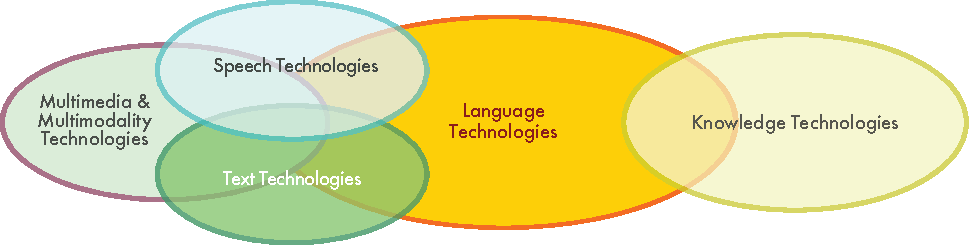
\includegraphics[width=\textwidth]{../_media/english/language_technologies}
  \caption{Language technology in context}
  \label{fig:ltincontext_en}
  \colorrule{grey3}{\textwidth}{1.5pt}
\end{figure*}

When we communicate, we combine language with other modes of communication and information media – for example speaking can involve gestures and facial expressions. Digital texts link to pictures and sounds. Movies may contain language in spoken and written form. In other words, speech and text technologies overlap and interact with other multimodal communication and multimedia technologies.

In this section, we will discuss the main application areas of language technology, i.\,e., language checking, web search, speech interaction, and machine translation. These applications and basic technologies include 

\begin{itemize}
\item spelling correction
\item authoring support
\item computer-assisted language learning
\item information retrieval 
\item information extraction
\item text summarisation
\item question answering
\item speech recognition 
\item speech synthesis 
\end{itemize}

\begin{figure*}[b]
  \colorrule{grey3}{\textwidth}{1.5pt}
  \center
  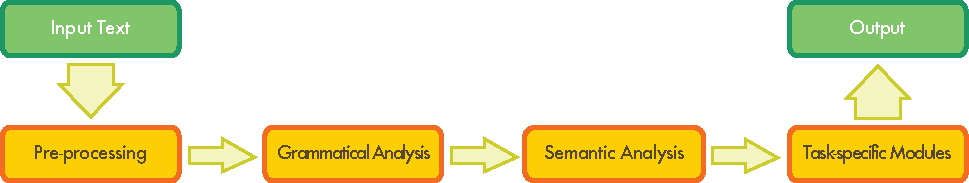
\includegraphics[width=\textwidth]{../_media/english/text_processing_app_architecture}
  \caption{A typical text processing architecture}
  \label{fig:textprocessingarch_en}
  \colorrule{grey3}{\textwidth}{1.5pt}
\end{figure*}

Language technology is an established area of research with an extensive set of introductory literature. The interested reader is referred to the following references:  \cite{jurafsky-martin01,manning-schuetze1,lt-world1,lt-survey1}.

Before discussing the above application areas, we will briefly describe the architecture of a typical LT system.

\subsection{Application Architectures}

Software applications for language processing typically consist of several components that mirror different aspects of language. While such applications are typically very complex, figure~\ref{fig:textprocessingarch_en} shows a highly simplified architecture of a typical text processing system. The first three modules handle the structure and meaning of the text input:

\begin{enumerate}
\item Pre-processing: cleans the data, analyses or removes formatting, detects the input languages, and so on.
\item Grammatical analysis: finds the verb, its objects, modifiers and other parts of speech; detects the sentence structure.
\item Semantic analysis: performs disambiguation (i.\,e., computes the appropriate meaning of words in a given context); resolves anaphora (i.\,e., which pronouns refer to which nouns in the sentence); represents the meaning of the sentence in a machine-readable way.
\end{enumerate}

After analysing the text, task-specific modules can perform other operations, such as automatic summarisation and database look-ups.

In the remainder of this section, we firstly introduce the core application areas for language technology, and follow this with a brief overview of the state of LT research and education today, and a description of past and present research programmes. Finally, we present an expert estimate of core LT tools and resources for Greek in terms of various dimensions such as availability, maturity and quality. The general situation of LT for the Greek language is summarised in a matrix (figure~\ref{fig:lrlttable_en}). Tools and resources that are boldfaced in the text can also be found in figure~\ref{fig:lrlttable_en} (p.~\pageref{fig:lrlttable_en}) at the end of this chapter. LT support for Greek is also compared to other languages that are part of this series.

\subsection{Core Application Areas}

In this section, we focus on the most important LT tools and resources, and provide an overview of LT activities in Greece.

\subsubsection{Language Checking}

\begin{figure*}[t]
  \colorrule{grey3}{\textwidth}{1.5pt}
  \center
  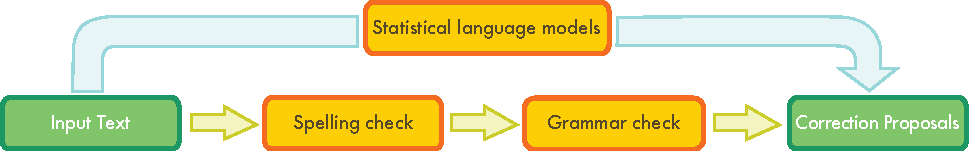
\includegraphics[width=\textwidth]{../_media/english/language_checking}
  \caption{Language checking (top: statistical; bottom: rule-based)}
  \label{fig:langcheckingaarch_en}
  \colorrule{grey3}{\textwidth}{1.5pt}
\end{figure*}

Anyone who has used a word processor such as Microsoft Word knows that it has a spell checker that highlights spelling mistakes and proposes corrections. The first spelling correction programs compared a list of extracted words against a dictionary of correctly spelled words. Today these programs are far more sophisticated. Using language-dependent algorithms for \textbf{grammatical analysis}, they detect errors related to morphology (e.\,g., plural formation) as well as syntax–related errors, such as a missing verb or a conflict of verb-subject agreement (e.\,g., \textit{she *write a letter}). However, most spell checkers will not find any errors in the following text \cite{zar1}:

\begin{quote}
  I have a spelling checker,\\
  It came with my PC.\\
  It plane lee marks four my revue\\
  Miss steaks aye can knot sea.
\end{quote}

For handling this type of errors, analysis of the context is needed in many cases, e.\,g., for deciding if a word is a verbal or a nominal type, as in the following example, where the inflected types λύσης (from the noun λύση [solution]) and λύσεις (from the verb λύνω [to solve]) coincide phonetically but differ in spelling and morphosyntactic identity:

\begin{itemize}
\item Μας παρουσίασε το σχέδιο της \textbf{λύσης}.
\item {[}He presented the solution plan to us.{]} 
\item Πρέπει να \textbf{λύσεις } αυτό το πρόβλημα.
\item {[}You must solve this problem.{]}
\end{itemize}

This type of analysis either needs to draw on language-specific \textbf{grammars} laboriously coded into the software by experts, or on a statistical language model. In this case, a model calculates the probability of a particular word as it occurs in a specific position (e.\,g., between the words that precede and follow it). For example: \textit{τις λύσεις} is a much more probable word sequence than * \textit{τις λύσης}. A statistical language model can be automatically created by using a large amount of (correct) language data, a \textbf{text corpus}. Most of these two approaches have been developed around data from English. However, they do not necessarily transfer straightforwardly to Greek with its flexible word order and rich inflection system.

\boxtext{Language checking is not limited to word processors but also applies to authoring systems.}

Language checking is not limited to word processors; it is also used in “authoring support systems”, i.\,e., software environments in which manuals and other types of technical documentation for complex IT, healthcare, engineering and other products, are written. To offset customer complaints about incorrect use and damage claims resulting from poorly understood instructions, companies are increasingly focusing on the quality of technical documentation while targeting the international market (via translation or localisation) at the same time. Advances in natural language processing have led to the development of authoring support software, which helps the writer of technical documentation to use vocabulary and sentence structures that are consistent with industry rules and (corporate) terminology restrictions.

Only few Greek organizations, companies and Language Service Providers offer products in this area. The Institute for Language and Speech Processing has developed a spelling and syntactic agreement checking module Symfonia (Agreement), for Greek language checking. A robust grammar checker for Greek is still missing.
Besides spell checkers and authoring support, language checking is also important in the field of computer-assisted language learning. Language checking applications also automatically correct search engine queries, as found in Google's \textit{Did you mean…} suggestions.

\subsubsection{Web Search}

\begin{figure*}[htb]
  \colorrule{grey3}{\textwidth}{1.5pt}
  \center
  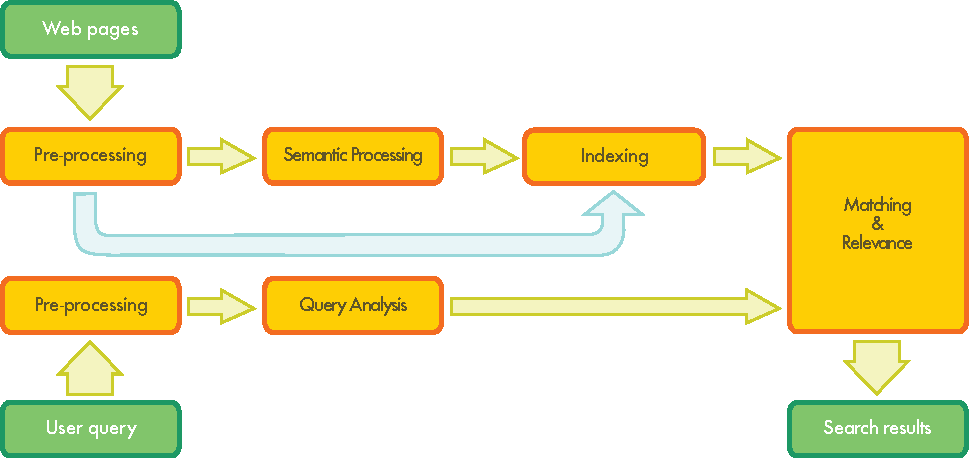
\includegraphics[width=\textwidth]{../_media/english/web_search_architecture}
  \caption{Web search}
  \label{fig:websearcharch_en}
  \colorrule{grey3}{\textwidth}{1.5pt}
 \end{figure*}

Searching the Web, intranets or digital libraries is probably the most widely used yet largely underdeveloped language technology application today. The Google search engine, which started in 1998, now handles about 80\% of all search queries \cite{spi1}. Since 2007, the verb \textit{γκουκγλάρω} or \textit{γκουγκλίζω} [to google] has even had an entry in some Greek dictionaries. The Google search interface and results page display has not significantly changed since the first version. However, in the current version, Google offers spelling correction for misspelled words and incorporates basic semantic search capabilities that can improve search accuracy by analysing the meaning of terms in a search query context \cite{pc1}. The Google success story shows that a large volume of data and efficient indexing techniques can deliver satisfactory results using a statistical approach to language processing. 

For more sophisticated information requests, it is essential to integrate deeper linguistic knowledge to facilitate text interpretation. Experiments using \textbf{lexical resources} such as machine-readable thesauri or ontological language resources (e.\,g., WordNet) have demonstrated improvements in finding pages using synonyms of the original search terms, such as \textit{ανανεώσιμες πηγές ενέργειας} {[}renewable energy resources{]}, \textit{αιολική ενέργεια} {[}wind power/energy{]}, or even more loosely related terms.

\boxtext{The next generation of search engines\\ will have to include much more sophisticated language technology.}

The next generation of search engines will have to include much more sophisticated language technology, escpecially to deal with search queries consisting of a question or other sentence type rather than a list of keywords. For the query, \textit{Give me a list of all companies that were taken over by other companies in the last five years}, a syntactic as well as \textbf{semantic analysis} is required. The system also needs to provide an index to quickly retrieve relevant documents. A satisfactory answer will require syntactic parsing to analyse the grammatical structure of the sentence and determine that the user wants companies that have been acquired, rather than companies that have acquired other companies. For the expression \textit{last five years}, the system needs to determine the relevant range of years, taking into account the present year. The query then needs to be matched against a huge amount of unstructured data to find the pieces of information that are relevant to the user’s request. This process is called information retrieval, and involves searching and ranking relevant documents. To generate a list of companies, the system also needs to recognise a particular string of words in a document represents a company name, using a process called named entity recognition.

A more demanding challenge is matching a query in one language with documents in another language. Cross-lingual information retrieval involves automatically translating the query into all possible source languages and then translating the results back into the user's target language.

Now that data is increasingly found in non-textual formats, there is a need for services that deliver multimedia information retrieval by searching images, audio files and video data. In the case of audio and video files, a speech recognition module must convert the speech content into text (or into a phonetic representation) that can then be matched against a user query.

\subsubsection{Speech Interaction}

Speech interaction is one of many application areas that depend on speech technology, i.\,e., technologies for processing spoken language. Speech interaction technology is used to create interfaces that enable users to interact in spoken language instead of using a graphical display, keyboard and mouse.  Today, these voice user interfaces (VUI) are used for partially or fully automated telephone services provided by companies to customers, employees or partners. Business domains that rely heavily on VUIs include banking, supply chain, public transportation, and telecommunications. Other uses of speech interaction technology include interfaces to car navigation systems and the use of spoken language as an alternative to the graphical or touchscreen interfaces in smartphones.

\begin{figure*}[htb]
  \colorrule{grey3}{\textwidth}{1.5pt}
  \center
  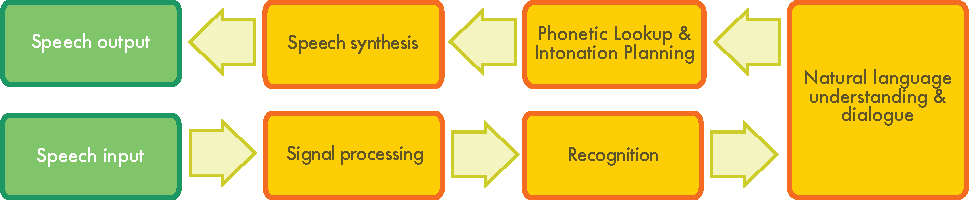
\includegraphics[width=\textwidth]{../_media/english/simple_speech-based_dialogue_architecture}
  \caption{Speech-based dialogue system}
  \label{fig:dialoguearch_en}
  \colorrule{grey3}{\textwidth}{1.5pt}
\end{figure*}

\begin{enumerate}
\item Automatic \textbf{speech recognition} (ASR) determines which words are actually spoken in a given sequence of sounds uttered by a user.  
\item Natural language understanding analyses the syntactic structure of a user’s utterance and interprets it according to the system in question.
\item Dialogue management determines which action to take given the user input and system functionality.   
\item \textbf{Speech synthesis} (text-to-speech or TTS) transforms the system’s reply into sounds for the user.
\end{enumerate}

One of the major challenges of ASR systems is to accurately recognise the words a user utters. This means restricting the range of possible user utterances to a limited set of keywords, or manually creating language models that cover a large range of natural language utterances. Using machine learning techniques, language models can also be generated automatically from \textbf{speech corpora}, i.\,e., large collections of speech audio files and text transcriptions. Restricting utterances usually forces people to use the voice user interface in a rigid way and can damage user acceptance; but the creation, tuning and maintenance of rich language models will significantly increase costs. VUIs that employ language models and initially allow a user to express their intent more flexibly — prompted by a \textit{How may I help you?} greeting — tend to be automated and are better accepted by users.

\boxtext{Speech interaction is the basis for interfaces that allow a user to interact with spoken language.}

Companies tend to use pre-recorded utterances by professional speakers for generating the output of the voice user interface. For static utterances where the wording does not depend on particular contexts of use or personal user data, this can deliver a rich user experience. But more dynamic content in an utterance may suffer from unnatural intonation because bits of audio files have simply been strung together. Through optimisation, today’s TTS systems are getting better at producing natural-sounding dynamic utterances.

Interfaces in speech interaction have been considerably standardised during the last decade in terms of their various technological components. There has also been strong market consolidation in speech recognition and speech synthesis. The national markets in the G20 countries (economically resilient countries with high populations) have been dominated by just five global players, with Nuance (USA) and Loquendo (Italy) being the most prominent players in Europe. In 2011, Nuance announced the acquisition of Loquendo, which represents a further step in market consolidation.

With regard to dialogue management technology and know-how, the market is dominated by national SME players. Rather than relying on a software license-driven product business, these companies are mainly positioned as full-service providers that create voice user interfaces as part of a system integration service. In the area of speech interaction, there is as yet no real market for syntactic and semantic analysis-based core technologies.

As for the actual employment of VUIs, demand in Greece has strongly increased within the last 5 years. This tendency has been driven by end customers’ increasing demand for customer self-service and the considerable cost optimisation aspect of automated telephone services, as well as by a significantly increased acceptance of spoken language as a modality for man-machine interaction. Such services are offered by SMEs which adapt and customize to Greek mixtures of imported technological solutions from big players as those mentioned above and indigenous technological solutions.

Looking ahead, there will be significant changes, due to the spread of smartphones as a new platform for managing customer relationships, in addition to fixed telephones, the Internet and e-mail. This will also affect how speech interaction technology is used. In the long term, there will be fewer telephone-based VUIs, and spoken language apps will play a far more central role as a user-friendly input for smartphones. This will be largely driven by stepwise improvements in the accuracy of speaker-independent speech recognition via the speech dictation services already offered as centralised services to smartphone users.

\subsubsection{Machine Translation}

The idea of using digital computers to translate natural languages can be traced back to 1946 and was followed by substantial funding for research during the 1950s and again in the 1980s. Yet \textbf{machine translation} (MT) still cannot deliver on its initial promise of providing across-the-board automated translation.

\boxtext{At its basic level, Machine Translation simply substitutes words in one natural language with words in another language.}

The most basic approach to machine translation is the automatic replacement of the words in a text written in one natural language with the equivalent words of another language. This can be useful in subject domains that have a very restricted, formulaic language such as weather reports. However, in order to produce a good translation of less restricted texts, larger text units (phrases, sentences, or even whole passages) need to be matched to their closest counterparts in the target language. The major difficulty is that human language is ambiguous. Ambiguity creates challenges on multiple levels, such as word sense disambiguation on the lexical level (a \textit{jaguar} is a brand of car or an animal) or the attachment of prepositional phrases on the syntactic level as in:

\begin{itemize}
\item[] The woman saw the car and her husband, too.
\item Die Frau sah das Auto und \textbf{ihr} Mann auch.
\item Die Frau sah das Auto und \textbf{ihren} Mann auch.
\end{itemize}

One way to build an MT system is to use linguistic rules. For translations between closely related languages, a translation using direct substitution may be feasible in cases such as the above example. However, rule-based (or linguistic knowledge-driven) systems often analyse the input text and create an intermediary symbolic representation from which the target language text can be generated. The success of these methods is highly dependent on the availability of extensive lexicons with morphological, syntactic, and semantic information, and large sets of grammar rules carefully designed by skilled linguists. This is a very long and therefore costly process.

\begin{figure*}[htb]
  \colorrule{grey3}{\textwidth}{1.5pt}
  \center
  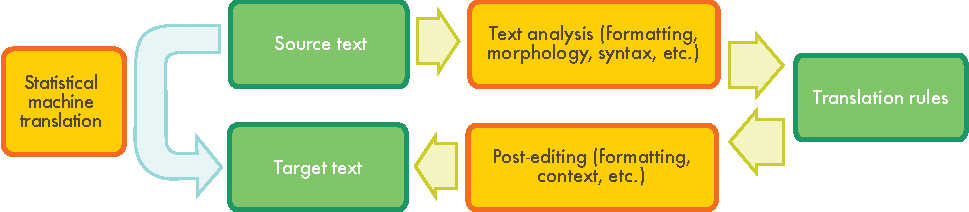
\includegraphics[width=\textwidth]{../_media/english/machine_translation}
  \caption{Machine translation (left: statistical; right: rule-based)}
  \label{fig:mtarch_en}
  \colorrule{grey3}{\textwidth}{1.5pt}
\end{figure*}
 
In the late 1980s when computational power increased and became cheaper, interest in statistical models for machine translation began to grow. Statistical models are derived from analysing bilingual text corpora, \textbf{parallel corpora}, such as the Europarl parallel corpus, which contains the proceedings of the European Parliament in 11 European languages. Given enough data, statistical MT works well enough to derive an approximate meaning of a foreign language text by processing parallel versions and finding plausible patterns of words. Unlike knowledge-driven systems, however, statistical (or data-driven) MT systems often generate ungrammatical output. Data-driven MT is advantageous because less human effort is required, and it can also cover special particularities of the language (e.\,g., idiomatic expressions) that are often ignored in knowledge-driven systems. 

The strengths and weaknesses of knowledge-driven and data-driven machine translation tend to be complementary, so that nowadays researchers focus on hybrid approaches that combine both methodologies. One such approach uses both knowledge-driven and data-driven systems, together with a selection module that decides on the best output for each sentence. However, results for sentences longer than, say, 12 words, will often be far from perfect. A more effective solution is to combine the best parts of each sentence from multiple outputs; this can be fairly complex, as corresponding parts of multiple alternatives are not always obvious and need to be aligned. 

Provided good adaptation in terms of user-specific terminology and workflow integration, the use of MT can increase productivity significantly. Language portals provide access to dictionaries and company-specific terminology, translation memory and MT support.

\boxtext{Machine Translation is particularly challenging for the Greek language.}

The quality of MT systems is still considered to have huge improvement potential. Challenges include the adaptability of the language resources to a given subject domain or user area and the integration into existing workflows with term bases and translation memories. In addition, most of the current systems are English-centred and support only few languages from and into Greek, which leads to frictions in the total translation workflow, and, e.\,g., forces MT users to learn different lexicon coding tools for different systems.

For Greek, MT is particularly challenging. Free word order poses problems for analysis, and extensive inflection is a challenge for generating words with proper gender and case markings. At the national level, there are small spin-off companies that try to gain a position in the market, by integrating Translation Memory and Statistical Machine Translation solutions, catering mostly for Greek paired with English, French and German.

Evaluation campaigns help to compare the quality of MT systems, the different approaches and the status of the systems for different language pairs. Figure~\ref{fig:euromatrix_de} (p.~\pageref{fig:euromatrix_de}), which was prepared during the EC Euromatrix+ project, shows the pair-wise performances obtained for 22 of the 23 official EU languages (Irish was not compared). The results are ranked according to a BLEU score, which indicates higher scores for better translations \cite{bleu1}. A human translator would normally achieve a score of around 80 points.

The best results (in green and blue) were achieved by languages that benefit from a considerable research effort in coordinated programmes and the existence of many parallel corpora (e.\,g., English, French, Dutch, Spanish and German). The languages with poorer results are shown in red. These languages either lack such development efforts or are structurally very different from other languages (e.\,g., Hungarian, Maltese and Finnish).

\subsection{Other Application Areas}

Building language technology applications involves a range of subtasks that do not always surface at the level of interaction with the user, but they provide significant service functionalities “behind the scenes” of the system in question. They all form important research issues that have now evolved into individual sub-disciplines of computational linguistics. Question answering, for example, is an active area of research for which annotated corpora have been built and scientific competitions have been initiated. The concept of question answering goes beyond keyword-based searches (in which the search engine responds by delivering a collection of potentially relevant documents) and enables users to ask a concrete question to which the system provides a single answer. For example:

\begin{itemize}
\item[] \textit{Question: How old was Neil Armstrong when he stepped on the moon?}
\item[] \textit{Answer: 38.}
\end{itemize}

While question answering is obviously related to the core area of web search, it is nowadays an umbrella term for such research issues as which different types of questions exist, and how they should be handled; how a set of documents that potentially contain the answer can be analysed and compared (do they provide conflicting answers?); and how specific information (the answer) can be reliably extracted from a document without ignoring the context. 

\boxtext{Language technology applications often provide significant service functionalities "behind the scenes" of larger software systems.}

Question answering is in turn related to information extraction (IE), an area that was extremely popular and influential when computational linguistics took a statistical turn in the early 1990s. IE aims to identify specific pieces of information in specific classes of documents, such as the key players in company takeovers as reported in newspaper stories. Another common scenario that has been studied is reports on terrorist incidents. The task here consists of mapping appropriate parts of the text to a template that specifies the perpetrator, target, time, location and results of the incident. Domain-specific template-filling is the central characteristic of IE, which makes it another example of a “behind the scenes” technology that forms a well-demarcated research area, which in practice needs to be embedded into a suitable application environment. 

Text summarisation and \textbf{text generation} are two borderline areas that can act either as standalone applications or play a supporting role. Summarisation attempts to give the essentials of a long text in a short form, and is one of the features available in Microsoft Word. It mostly uses a statistical approach to identify the “important” words in a text (i.\,e., words that occur very frequently in the text in question but less frequently in general language use) and determine which sentences contain the most of these “important” words. These sentences are then extracted and put together to create the summary. In this very common commercial scenario, summarisation is simply a form of sentence extraction, and the text is reduced to a subset of its sentences. An alternative approach, for which some research has been carried out, is to generate brand new sentences that do not exist in the source text. 

\boxtext{For the Greek language, research in most text technologies is much less developed than for the English language.}

This requires a deeper understanding of the text, which means that so far this approach is far less robust. On the whole, a text generator is rarely used as a stand-alone application but is embedded into a larger software environment, such as a clinical information system that collects, stores and processes patient data. Creating reports is just one of many applications for text summarisation. 
For Greek, the situation in all these research areas is much less developed than it is for English, where question answering, information extraction, and summarization have since the 1990s been the subject of numerous open competitions, primarily those organized by DARPA/NIST in the United States. These have significantly improved the state of the art, but the focus has always been on English; some competitions have added multilingual tracks, but Greek was never prominent. However, text engineering platforms like ELLOGON have been developed, mostly inspired by (and catering for) information extraction as well as text and media analytics related applications. Small spin-offs are active in application areas such as media (TV, Radio, Web) monitoring, sentiment analysis and opinion mining etc., focusing on Greek and English content

Summarization systems, when using purely statistical methods, are often language-independent to a good extent, and thus some research prototypes are available. For text generation, reusable components have traditionally been limited to the surface realization modules (the 'generation grammars'); again, most available software is for English.

Apart from the intricacies of language as a communication medium in general, natural language processing for a less-widely spoken language like Greek poses its own challenges. Research endeavours focused on Greek try to model language phenomena on the one hand and develop useful applications on the other. This is reflected in the relatively high number of research groups and researchers trying to attack language processing problems from the morphographemic and phonetic level to technological solutions for access to information and content.

\subsection{Educational Programmes}

Language Technology is a highly interdisciplinary field, involving the expertise of linguists, computer scientists, mathematicians, philosophers, psycholinguists, and neuroscientists, among others. In Greece there is only one dedicated post-graduate programme that deals with Language Technology. This programme is offered jointly by the National Kapodistrian University of Athens and the National Technical University of Athens, while lectures are given by members of these two Universities and of the two main research Labs on LT, namely ILSP / R.C ‘Athena’ and the Software and Knowledge Engineering Laboratory of NCSR Demokritos. Approximately 35 students graduate from this programme every two years since 1998.

Isolated courses on Computational Linguistics and related areas are offered by all other major Greek Universities both in their un-dergraduate and postgraduate curricula (most notable cases among those are the Athens University for Economics and Business, the University of Pireaus, the University of Patras, the Aristotle University of Thessaloniki). Many of these programs and courses have only recently been introduced.

The increasing number of new research groups and labs in Universities and research centres focussing on LT, indicates the impetus of the field and the popularity it has been gaining among students.

The Institute for Language and Speech Processing and the Institute for Informatics and Telecommunications of the NCSR Demokritos are the two major Research Institutes that routinely offer opportunities for internships to students of Computational Linguistics and related fields.

There are no data available on the number of students that study on both under- and post-graduate levels in fields related to Language Technology. Most people that wish to pursue education in these fields do so in Universities and specialized Centers abroad. Most industrial and academic positions related to Language Tech-nologies are occupied by people that have already studied and/or worked abroad. Due to the lack of adequately qualified personnel, in many cases jobs that need Language Technology expertise are filled by computer engineers that have a (short or more extensive) LT (self)training.

\subsection[National Projects and Initiatives]{National Projects\newline and Initiatives}

The existence of LT industry in Greece can be traced back to major LT programs carried out in the last decades. The first such program was EUROTRA, an ambitious Machine Translation (MT) project established and funded by the European Commission from the late 1970s until 1994. Even though the EUROTRA project did not fulfill the expectations of creating a state-of-the-art MT system, the project had a long-term impact on the language industries in Europe; an additional result of this project was the creation and training of a critical mass of scientists, researchers in the emerging field. 

National programmes (mainly funded through EU Structural Funds) in the '90s and early '00s aimed at the development of language technology and the creation of infrastructure in the field of language and speech processing (text corpora, speech databases, speech and written language processing tools, computational lexica, electronic dictionaries, educational platforms for teaching Greek). These programmes (namely STRIDE, DIALOGOS, EPET I – LT, EPET II) were seminal for the continuation of the field of LT in the country and together with EU projects in the 1990s and early 2000 catered for the creation of the basic tools and technologies for the mark-up and annotation of language resources for Greek.

Follow-up programmes, such as 'SOUND, IMAGE, LANGUAGE', were more user- and application-oriented. They focused on the use of contemporary Language Technology in sectors like Digital Cultural Heritage, e-Government, and multimedia content processing for the mass media communication industry.

A significant asset gained by those funding initiatives is the establishment of a group of LT teams in major Research Centers and University labs as well as of LT-aware teams in companies. Most of these teams are continuously active in the area through EU research activities and have acted positively in producing most of the LT resources and tools that are now available for Greek, covering the axes of text, speech and multimedia data processing.

A new national all-areas R\&D funding initiative (SYNERGASIA) is currently unfolding, including some promising LT projects - not focusing, however, on LT. Since this programme is built to foster academia-industry collaborations, it is foreseen that a good set of Greek language tools and LT enhanced systems and services will be available in the coming years.

Still, public funding for LT projects in Greece is relatively low compared to the expenses spent on issues like translation and multilingual information access by the USA \cite{laz2}. An additional crucial fact is that private R\&D funding in Greece is overall extremely low, a fact that proves especially disad-vantageous for technologies like LT.

\subsection{The Private Sector}

Indicative of the significance of LT in Greece is the existence of a small, but important for the size of the country, number of private companies, spin-off companies included, which conduct state-of-the-art research in the fields of speech recognition and synthesis, media monitoring, machine translation, language resources pro-duction (dictionaries, thesauri, ontologies), ePublishing, eLearning and intelligent content analysis.

Focus on development for these companies lies on providing add-ons and advanced search engines for special-interest portals by exploiting topic-relevant semantics. Due to the still high demands in processing power, such search engines are only economically usable on relatively small text corpora. Processing time easily exceeds that of a common statistical search engine as, e.\,g., provided by Google by a magnitude of thousands. These search engines also have high demand in topic-specific domain modelling, making it not feasible to use these mechanisms on web scale.

\subsection{Availability of Tools and Resources}

A good part of the basic LRT components have been developed for Greek: language resources (mono- and multilingual, multimodal etc.) computational lexica, parsers, spelling and syntax checkers, named entity recognizers, semantic annotators, translation applications, authoring tools, speech recognition and synthesis technologies, language technology assisted educational software -- a broad range. It is obvious, however, that the field needs further development.

Some products have reached the market, with ranging success. Services offered over the internet concerning language resources include monolingual Greek corpora (The Hellenic National Corpus, the Corpus of Greek Texts, and the CGL newspaper corpus). The market, though, continues to be small and not well aware of the availability.

Figure~\ref{fig:lrlttable_en} provides a rating for language technology support for the Greek language. This rating of existing tools and resources was generated by leading experts in the field who provided estimates based on a scale from 0 (very low) to 6 (very high) using seven criteria.

\begin{figure*}[htb]
\centering
%\begin{tabular}{>{\columncolor{orange1}}p{.33\linewidth}ccccccc} % ORIGINAL
\begin{tabular}{>{\columncolor{orange1}}p{.33\linewidth}@{\hspace*{6mm}}c@{\hspace*{6mm}}c@{\hspace*{6mm}}c@{\hspace*{6mm}}c@{\hspace*{6mm}}c@{\hspace*{6mm}}c@{\hspace*{6mm}}c}
\rowcolor{orange1}
 \cellcolor{white}&\begin{sideways}\makecell[l]{Quantity}\end{sideways}
&\begin{sideways}\makecell[l]{\makecell[l]{Availability} }\end{sideways} &\begin{sideways}\makecell[l]{Quality}\end{sideways}
&\begin{sideways}\makecell[l]{Coverage}\end{sideways} &\begin{sideways}\makecell[l]{Maturity}\end{sideways} &\begin{sideways}\makecell[l]{Sustainability}\end{sideways} &\begin{sideways}\makecell[l]{Adaptability}\end{sideways} \\ \addlinespace
\multicolumn{8}{>{\columncolor{orange2}}l}{Language Technology: Tools, Technologies and Applications} \\ \addlinespace
Speech Recognition	&3&2&4&3&5&4&3 \\ \addlinespace
Speech Synthesis &4&2&5&4&5&4&3\\ \addlinespace
Grammatical analysis &2&1.5&3.5&3&3&3&3\\ \addlinespace
Semantic analysis &1&1.5&1.5&1.5&1.5&1.5&1.5\\ \addlinespace
Text generation &1&1&2&1&1&1&1\\ \addlinespace
Machine translation &2&1&1&1&1&1&2\\ \addlinespace
\multicolumn{8}{>{\columncolor{orange2}}l}{Language Resources: Resources, Data and Knowledge Bases} \\ \addlinespace
Text corpora &3&3.5&3.5&3&3&4&4\\ \addlinespace
Speech corpora &2&1&3&2&3&2&2\\ \addlinespace
Parallel corpora &2&2&2&2&3&3&2\\ \addlinespace
Lexical resources &1.5&1&2.5&2&2&2.5&2.5\\ \addlinespace
Grammars &1&1&1&1&1&2&1\\
\end{tabular}
\caption{State of language technology support for Greek}
\label{fig:lrlttable_en}
\end{figure*}

The key results for the Greek language technology can be summed up as follows:

\begin{itemize}
\item While some corpora of high quality exist, covering mainly Modern Greek, Greek reference corpora are well below the 100 million threshold and mainly include journalistic texts, whereas spoken text types are found only in few. 
\item All of the corpora are accessed over the Internet and are not downloadable. 
\item Most LRs developed for the Greek language have not been sufficiently maintained and/or updated once constructed. 
\item Many of the resources lack standardization, i.\,e., even if they exist, sustainability is not given; concerted programs and initiatives are needed to standardize data and interchange formats. 
\item Semantics is more difficult to process than syntax; text semantics is more difficult to process than word and sentence semantics.
\item The more semantics a tool takes into account, the more difficult it is to find the right data; more efforts for supporting deep processing are needed.
\item Standards do exist for semantics in the sense of world knowledge (RDF, OWL, etc.); they are, however, not easily applicable to NLP tasks.
\item Speech processing is currently more mature than NLP for written text. 
\item In what concerns lexical resources, in terms of \textit{quantity} and \textit{variety}, there is a great need for more lexicons with semantic and syntactic information, semantic networks, terminological data for different domains, as well as more bilingual (for pairs of languages other than Greek-English) and multilingual resources. As regards \textit{maturity}, very few are mature enough to be directly integrated in NLP tools and systems. 
\item Research was successful in designing particular high quality software, but it is nearly impossible to come up with sustainable and standardized solutions given the current funding situations. 
\item Tools are at varied levels of maturity, from lab prototype to market product. 
\item Documentation of resources and tools is scarce. 
\item Greek multimedia/ multimodal resources present a large variety and a satisfactory coverage regarding genres, media and modalities. 
\item In general, syntactically and semantically annotated corpora are rather under-represented while at the same time the existing resources reach high levels of quality. 
\end{itemize}

\subsection{Cross-language comparison}

The current state of LT support varies considerably from one language community to another. In order to compare the situation between languages, this section will present an evaluation based on two sample application areas (machine translation and speech processing) and one underlying technology (text analysis), as well as basic resources needed for building LT applications. The languages were categorised using the following five-point scale: 

\begin{enumerate}
\item Excellent support
\item Good support
\item Moderate support
\item Fragmentary support
\item Weak or no support
\end{enumerate}

LT support was measured according to the following criteria:

\textbf{Speech Processing:} Quality of existing speech recognition technologies, quality of existing speech synthesis technologies, coverage of domains, number and size of existing speech corpora, amount and variety of available speech-based applications.

\textbf{Machine Translation:} Quality of existing MT technologies, number of language pairs covered, coverage of linguistic phenomena and domains, quality and size of existing parallel corpora, amount and variety of available MT applications.

\textbf{Text Analysis:} Quality and coverage of existing text analysis technologies (morphology, syntax, semantics), coverage of linguistic phenomena and domains, amount and variety of available applications, quality and size of existing (annotated) text corpora, quality and coverage of existing lexical resources (e.\,g., WordNet) and grammars.

\textbf{Resources:} Quality and size of existing text corpora, speech corpora and parallel corpora, quality and coverage of existing lexical resources and grammars.

Figures~\ref{fig:speech_cluster_en} to~\ref{fig:resources_cluster_en} show that language technology for Greek has indeed progressed over the past decades. It has not, however, reached the status of the bigger languages (bigger in terms of numbers of speakers and in available resources). This is due to many factors; to name a linguistic one, the identity of the language (unique alphabet, difficult morphology) demands the development of language tools especially tailored to Greek, which, in turn, hampers technology transfer from other languages. It is obvious that Greek has not yet reached the quality and coverage of comparable resources and tools for the English language, which is in the lead in almost all LT areas. And there are still plenty of gaps in English language resources with regard to high quality applications.

Specific speech processing technologies (e.\,g., text-to-speech) perform well enough to be successfully integrated into a number of industrial applications. Today’s text analysis components and language resources  cover the linguistic phenomena of Greek to a certain extent and form part of many applications involving mostly shallow natural language processing, e.\,g., spelling correction and authoring support.

However, for building more sophisticated applications, such as machine translation, there is a clear need for resources and technologies that cover a wider range of linguistic aspects and allow a deep semantic analysis of the input text. By improving the quality and coverage of these basic resources and technologies, we shall be able to open up new opportunities for tackling a vast range of advanced application areas, including high-quality machine translation.

\subsection{Conclusions}

\emph{In this series of white papers, we have made an important effort by assessing the language technology support for 30 European languages, and by providing a high-level comparison across these languages. By identifying the gaps, needs and deficits, the European language technology community and its related stakeholders are now in a position to design a large scale research and development programme aimed at building a truly multilingual, technology-enabled communication across Europe.}

The results of this white paper series show that there is a dramatic difference in language technology support for the various European languages. While there are good quality software and resources available for some languages and application areas, others, usually smaller languages, have substantial gaps. Many languages lack basic technologies for text analysis and the essential resources. Others have basic tools and resources but the implementation of for example semantic methods is still far away. Therefore a large-scale effort is needed to attain the ambitious goal of providing high-quality language technology support for all European languages, for example through high quality machine translation. 

In the case of the Greek language, although we witnessed the progress of the field, we cannot but state that there is a lot to be done as regards the current state of language technology support. The LT research community in Greece has been supported in the past by national and European research programmes, which have resulted in a number of large-scale resources and state-of-the-art technologies. However, the scope of the resources and the range of tools are still very limited when compared to the resources and tools for the English language, and they are simply not sufficient in quality and quantity to develop the kind of technologies required to support a truly multilingual knowledge society.

Nor can we simply transfer technologies already developed and optimised for the English language to handle Greek. English-based systems for parsing (syntactic and grammatical analysis of sentence structure) typically perform far less well on Greek texts, due to the specific characteristics of the Greek language.

Greece never could claim the existence of language technology industry dedicated to transforming research into products. The few companies that were active in this domain have either stopped or severely cut their LT efforts, leaving the field to a number of specialized SMEs that are not robust enough to address the internal and the global market with a sustained strategy. 

Our findings show that the only alternative is to make a substantial effort to create LT resources for Greek, and use them to drive forward research, innovation and development. The need for large amounts of data and the extreme complexity of language technology systems makes it vital to develop a new infrastructure and a more coherent research organization to spur greater sharing and cooperation.

There is also a lack of continuity in research and development funding. Short-term coordinated programmes tend to alternate with periods of sparse or zero funding at the national level. In addition, there is an overall lack of coordination with programmes in other EU countries and at the European Commission level.

We can therefore conclude that there is a desperate need for a large, coordinated initiative focused on overcoming the differences in language technology readiness for European languages as a whole.

The long term goal of META-NET is to enable the creation of high-quality language technology for all languages. This requires all stakeholders - in politics, research, business, and society - to unite their efforts. The resulting technology will help tear down existing barriers and build bridges between Europe’s languages, paving the way for political and economic unity through cultural diversity. 
\end{multicols}

\clearpage

\begin{figure*}[t]
  \small
  \centering
  \begin{tabular}
  { % defines color for each column.
  >{\columncolor{corange5}}p{.13\linewidth}@{\hspace{.040\linewidth}}
  >{\columncolor{corange4}}p{.13\linewidth}@{\hspace{.040\linewidth}}
  >{\columncolor{corange3}}p{.13\linewidth}@{\hspace{.040\linewidth}}
  >{\columncolor{corange2}}p{.13\linewidth}@{\hspace{.040\linewidth}}
  >{\columncolor{corange1}}p{.13\linewidth} 
  }
  \multicolumn{1}{>{\columncolor{white}}c@{\hspace{.040\linewidth}}}{\textbf{Excellent}} & 
  \multicolumn{1}{@{}>{\columncolor{white}}c@{\hspace{.040\linewidth}}}{\textbf{Good}} &
  \multicolumn{1}{@{}>{\columncolor{white}}c@{\hspace{.040\linewidth}}}{\textbf{Moderate}} &
  \multicolumn{1}{@{}>{\columncolor{white}}c@{\hspace{.040\linewidth}}}{\textbf{Fragmentary}} &
  \multicolumn{1}{@{}>{\columncolor{white}}c}{\textbf{Weak/no}} \\ 
  \multicolumn{1}{>{\columncolor{white}}c@{\hspace{.040\linewidth}}}{\textbf{support}} & 
  \multicolumn{1}{@{}>{\columncolor{white}}c@{\hspace{.040\linewidth}}}{\textbf{support}} &
  \multicolumn{1}{@{}>{\columncolor{white}}c@{\hspace{.040\linewidth}}}{\textbf{support}} &
  \multicolumn{1}{@{}>{\columncolor{white}}c@{\hspace{.040\linewidth}}}{\textbf{support}} &
  \multicolumn{1}{@{}>{\columncolor{white}}c}{\textbf{support}} \\ \addlinespace
  
& \vspace*{0.5mm}English
& \vspace*{0.5mm}
Czech \newline 
Dutch \newline 
Finnish \newline 
French \newline 
German \newline   
Italian \newline  
Portuguese \newline 
Spanish \newline
& \vspace*{0.5mm}Basque \newline 
Bulgarian \newline 
Catalan \newline 
Danish \newline 
Estonian \newline 
Galician\newline 
Greek \newline  
Hungarian  \newline
Irish \newline  
Norwegian \newline 
Polish \newline 
Serbian \newline 
Slovak \newline 
Slovene \newline 
Swedish \newline
& \vspace*{0.5mm}
Croatian \newline 
Icelandic \newline  
Latvian \newline 
Lithuanian \newline 
Maltese \newline 
Romanian\\
\end{tabular}
\caption{Speech processing: state of language technology support for 30 European languages}
\label{fig:speech_cluster_en}
\end{figure*}

\begin{figure*}[b]
  \small
  \centering
  \begin{tabular}
  { % defines color for each column.
  >{\columncolor{corange5}}p{.13\linewidth}@{\hspace{.040\linewidth}}
  >{\columncolor{corange4}}p{.13\linewidth}@{\hspace{.040\linewidth}}
  >{\columncolor{corange3}}p{.13\linewidth}@{\hspace{.040\linewidth}}
  >{\columncolor{corange2}}p{.13\linewidth}@{\hspace{.040\linewidth}}
  >{\columncolor{corange1}}p{.13\linewidth} 
  }
  \multicolumn{1}{>{\columncolor{white}}c@{\hspace{.040\linewidth}}}{\textbf{Excellent}} & 
  \multicolumn{1}{@{}>{\columncolor{white}}c@{\hspace{.040\linewidth}}}{\textbf{Good}} &
  \multicolumn{1}{@{}>{\columncolor{white}}c@{\hspace{.040\linewidth}}}{\textbf{Moderate}} &
  \multicolumn{1}{@{}>{\columncolor{white}}c@{\hspace{.040\linewidth}}}{\textbf{Fragmentary}} &
  \multicolumn{1}{@{}>{\columncolor{white}}c}{\textbf{Weak/no}} \\ 
  \multicolumn{1}{>{\columncolor{white}}c@{\hspace{.040\linewidth}}}{\textbf{support}} & 
  \multicolumn{1}{@{}>{\columncolor{white}}c@{\hspace{.040\linewidth}}}{\textbf{support}} &
  \multicolumn{1}{@{}>{\columncolor{white}}c@{\hspace{.040\linewidth}}}{\textbf{support}} &
  \multicolumn{1}{@{}>{\columncolor{white}}c@{\hspace{.040\linewidth}}}{\textbf{support}} &
  \multicolumn{1}{@{}>{\columncolor{white}}c}{\textbf{support}} \\ \addlinespace
  
& \vspace*{0.5mm} English 
& \vspace*{0.5mm} 
French \newline 
Spanish
& \vspace*{0.5mm}
Catalan \newline 
Dutch \newline 
German \newline 
Hungarian \newline
Italian \newline 
Polish \newline 
Romanian \newline 
& \vspace*{0.5mm}Basque \newline 
Bulgarian \newline 
Croatian \newline 
Czech \newline
Danish \newline 
Estonian \newline 
Finnish \newline 
Galician \newline 
Greek \newline 
Icelandic \newline 
Irish \newline 
Latvian \newline 
Lithuanian \newline 
Maltese \newline 
Norwegian \newline 
Portuguese \newline 
Serbian \newline 
Slovak \newline 
Slovene \newline 
Swedish \newline 
\end{tabular}
\caption{Machine translation: state of language technology support for 30 European languages}
\label{fig:mt_cluster_en}
\end{figure*}

\begin{figure*}[t]
  \small
  \centering
  \begin{tabular}
  { % defines color for each column.
  >{\columncolor{corange5}}p{.13\linewidth}@{\hspace{.040\linewidth}}
  >{\columncolor{corange4}}p{.13\linewidth}@{\hspace{.040\linewidth}}
  >{\columncolor{corange3}}p{.13\linewidth}@{\hspace{.040\linewidth}}
  >{\columncolor{corange2}}p{.13\linewidth}@{\hspace{.040\linewidth}}
  >{\columncolor{corange1}}p{.13\linewidth} 
  }
  \multicolumn{1}{>{\columncolor{white}}c@{\hspace{.040\linewidth}}}{\textbf{Excellent}} & 
  \multicolumn{1}{@{}>{\columncolor{white}}c@{\hspace{.040\linewidth}}}{\textbf{Good}} &
  \multicolumn{1}{@{}>{\columncolor{white}}c@{\hspace{.040\linewidth}}}{\textbf{Moderate}} &
  \multicolumn{1}{@{}>{\columncolor{white}}c@{\hspace{.040\linewidth}}}{\textbf{Fragmentary}} &
  \multicolumn{1}{@{}>{\columncolor{white}}c}{\textbf{Weak/no}} \\ 
  \multicolumn{1}{>{\columncolor{white}}c@{\hspace{.040\linewidth}}}{\textbf{support}} & 
  \multicolumn{1}{@{}>{\columncolor{white}}c@{\hspace{.040\linewidth}}}{\textbf{support}} &
  \multicolumn{1}{@{}>{\columncolor{white}}c@{\hspace{.040\linewidth}}}{\textbf{support}} &
  \multicolumn{1}{@{}>{\columncolor{white}}c@{\hspace{.040\linewidth}}}{\textbf{support}} &
  \multicolumn{1}{@{}>{\columncolor{white}}c}{\textbf{support}} \\ \addlinespace

& \vspace*{0.5mm}English
& \vspace*{0.5mm}
  Dutch \newline 
  French \newline 
  German \newline 
  Italian \newline 
  Spanish
& \vspace*{0.5mm}Basque \newline 
  Bulgarian \newline 
  Catalan \newline 
  Czech \newline 
  Danish \newline 
  Finnish \newline 
  Galician \newline 
  Greek \newline 
  Hungarian \newline 
  Norwegian \newline 
  Polish \newline 
  Portuguese \newline 
  Romanian \newline 
  Slovak \newline 
  Slovene \newline 
  Swedish \newline 
& \vspace*{0.5mm}
  Croatian \newline 
  Estonian \newline 
  Icelandic \newline 
  Irish \newline 
  Latvian \newline 
  Lithuanian \newline 
  Maltese \newline 
  Serbian \\
  \end{tabular}
\caption{Text analysis: state of language technology support for 30 European languages}
\label{fig:text_cluster_en}
\end{figure*}

\begin{figure*}[b]
  \small
  \centering
  \begin{tabular}
  { % defines color for each column.
  >{\columncolor{corange5}}p{.13\linewidth}@{\hspace{.040\linewidth}}
  >{\columncolor{corange4}}p{.13\linewidth}@{\hspace{.040\linewidth}}
  >{\columncolor{corange3}}p{.13\linewidth}@{\hspace{.040\linewidth}}
  >{\columncolor{corange2}}p{.13\linewidth}@{\hspace{.040\linewidth}}
  >{\columncolor{corange1}}p{.13\linewidth} 
  }
  \multicolumn{1}{>{\columncolor{white}}c@{\hspace{.040\linewidth}}}{\textbf{Excellent}} & 
  \multicolumn{1}{@{}>{\columncolor{white}}c@{\hspace{.040\linewidth}}}{\textbf{Good}} &
  \multicolumn{1}{@{}>{\columncolor{white}}c@{\hspace{.040\linewidth}}}{\textbf{Moderate}} &
  \multicolumn{1}{@{}>{\columncolor{white}}c@{\hspace{.040\linewidth}}}{\textbf{Fragmentary}} &
  \multicolumn{1}{@{}>{\columncolor{white}}c}{\textbf{Weak/no}} \\ 
  \multicolumn{1}{>{\columncolor{white}}c@{\hspace{.040\linewidth}}}{\textbf{support}} & 
  \multicolumn{1}{@{}>{\columncolor{white}}c@{\hspace{.040\linewidth}}}{\textbf{support}} &
  \multicolumn{1}{@{}>{\columncolor{white}}c@{\hspace{.040\linewidth}}}{\textbf{support}} &
  \multicolumn{1}{@{}>{\columncolor{white}}c@{\hspace{.040\linewidth}}}{\textbf{support}} &
  \multicolumn{1}{@{}>{\columncolor{white}}c}{\textbf{support}} \\ \addlinespace
    
& \vspace*{0.5mm}English
& \vspace*{0.5mm} 
    Czech \newline 
    Dutch \newline 
    French \newline 
    German \newline 
    Hungarian \newline
    Italian \newline
    Polish \newline
    Spanish \newline
    Swedish \newline 
& \vspace*{0.5mm} Basque\newline 
    Bulgarian\newline 
    Catalan \newline 
    Croatian \newline 
    Danish \newline 
    Estonian \newline 
    Finnish \newline 
    Galician \newline 
    Greek \newline 
    Norwegian \newline 
    Portuguese \newline 
    Romanian \newline 
    Serbian \newline 
    Slovak \newline 
    Slovene \newline
&  \vspace*{0.5mm}
    Icelandic \newline 
    Irish \newline 
    Latvian \newline 
    Lithuanian \newline 
    Maltese  \\
  \end{tabular}
  \caption{Speech and text resources: State of support for 30 European languages}  
  \label{fig:resources_cluster_en}
\end{figure*}

\clearpage

% --------------------------------------------------------------------------
\ssection[About META-NET]{About META-NET}

\begin{multicols}{2}
META-NET is a Network of Excellence funded by the European Commission. The network currently consists of 54 members from 33 European countries \cite{rehm2011}. META-NET fosters the Multilingual Europe Technology Alliance (META), a growing community of language technology professionals and organisations in Europe. META-NET cooperates with other initiatives like the Common Language Resources and Technology Infrastructure (CLARIN), which is helping establish digital humanities research in Europe. META-NET fosters the technological foundations for a truly multilingual European information society that:

\begin{itemize}
\item makes communication and cooperation possible across languages;
\item provides equal access to information and knowledge in any language;
\item offers advanced and affordable networked information technology to European citizens.
\end{itemize}

META-NET stimulates and promotes multilingual technologies for all European languages. The technologies enable automatic translation, content production, information processing and knowledge management for a wide variety of applications and subject domains. The network wants to improve current approaches, so better communication and cooperation across languages can take place. Europeans have an equal right to information and knowledge regardless of language.

META-NET launched on 1 February 2010 with the goal of advancing research in language technology (LT). The network supports a Europe that unites as a single digital market and information space. META-NET has conducted several activities that further its goals. META-VISION, META-SHARE and META-RESEARCH are the network’s three lines of action.

\textbf{META-VISION} fosters a dynamic and influential stakeholder community that unites around a shared vision and a common strategic research agenda (SRA). The main focus of this activity is to build a coherent and cohesive LT community in Europe by bringing together representatives from highly fragmented and diverse groups of stakeholders. In the first year of META-NET, presentations at the FLaReNet Forum (Spain), Language Technology Days (Luxembourg), JIAMCATT 2010 (Luxembourg), LREC 2010 (Malta), EAMT 2010 (France) and ICT 2010 (Belgium) centred on public outreach. According to initial estimates, META-NET has already contacted more than 2,500 LT professionals to develop its goals and visions with them. At the META-FORUM 2010 event in Brussels, META-NET communicated the initial results of its vision building process to more than 250 participants. In a series of interactive sessions, the participants provided feedback on the visions presented by the network. 

\textbf{META-SHARE} creates an open, distributed facility for exchanging and sharing resources. The peer-to-peer network of repositories will contain language data, tools and web services that are documented with high-quality metadata and organised in standardised categories. The resources can be readily accessed and uniformly searched. The available resources include free, open source materials as well as restricted, commercially available, fee-based items. META-SHARE targets existing language data, tools and systems as well as new and emerging products that are required for building and evaluating new technologies, products and services. The reuse, combination, repurposing and re-engineering of language data and tools plays a crucial role. META-SHARE will eventually become a critical part of the LT marketplace for developers, localisation experts, researchers, translators and language professionals from small, mid-sized and large enterprises. META-SHARE addresses the full development cycle of LT—from research to innovative products and services. A key aspect of this activity is establishing META-SHARE as an important and valuable part of a European and global infrastructure for the LT community. 

\textbf{META-RESEARCH} builds bridges to related technology fields. This activity seeks to leverage advances in other fields and to capitalise on innovative research that can benefit language technology. In particular, this activity wants to bring more semantics into machine translation (MT), optimise the division of labour in hybrid MT, exploit context when computing automatic translations and prepare an empirical base for MT. META-RESEARCH is working with other fields and disciplines, such as machine learning and the Semantic Web community. META-RESEARCH focuses on collecting data, preparing data sets and organising language resources for evaluation purposes; compiling inventories of tools and methods; and organising workshops and training events for members of the community. This activity has already clearly identified aspects of MT where semantics can impact current best practices. In addition, the activity has created recommendations on how to approach the problem of integrating semantic information in MT. META-RESEARCH is also finalising a new language resource for MT, the Annotated Hybrid Sample MT Corpus, which provides data for English-German, English-Spanish and English-Czech language pairs. META-RESEARCH has also developed software that collects multilingual corpora that are hidden on the Web.
\end{multicols}

\vfill
\centerline{office@meta-net.eu -- http://www.meta-net.eu}

\cleardoublepage

\selectlanguage{english}

\appendix
\addtocontents{toc}{\protect\bigskip}

\selectlanguage{english}\bsection[Παραπομπές -- References]{Παραπομπές --- References}
\bibliographystyle{unsrt}
\bibliography{greek_references}
  
\cleardoublepage

\selectlanguage{english}\bsection[Μέλη του META-NET -- META-NET Members]{Μέλη του META-NET --- META-NET Members}
\label{metanetmembers}

\small
\begin{longtable}{@{}llp{113mm}@{}}
  Αυστρία & \textcolor{grey1}{Austria} & Zentrum für Translationswissenschaft, Universität Wien: Gerhard Budin\\ \addlinespace 
  Βέλγιο & \textcolor{grey1}{Belgium} & Computational Linguistics and Psycholinguistics Research Centre, University of Antwerp: Walter Daelemans\\ \addlinespace
  & & Centre for Processing Speech and Images, University of Leuven: Dirk van Compernolle \\ \addlinespace
  Βουλγαρία & \textcolor{grey1}{Bulgaria} & Institute for Bulgarian Language, Bulgarian Academy of Sciences: Svetla Koeva \\ \addlinespace
  Γαλλία & \textcolor{grey1}{France} & Centre National de la Recherche Scientifique, Laboratoire d'Informatique pour la Mécanique et les Sciences de l'Ingénieur and Institute for Multilingual and Multimedia Information: Joseph Mariani \\ \addlinespace
  & & Evaluations and Language Resources Distribution Agency: Khalid Choukri\\ \addlinespace 
  Γερμανία & \textcolor{grey1}{Germany} & Language Technology Lab, DFKI: Hans Uszkoreit, Georg Rehm\\ \addlinespace
  & & Human Language Technology and Pattern Recognition, RWTH Aachen University: Hermann Ney \\ \addlinespace
  & & Department of Computational Linguistics, Saarland University: Manfred Pinkal\\ \addlinespace Δανία &  \textcolor{grey1}{Denmark} & Centre for Language Technology, University of Copenhagen: \newline Bolette Sandford Pedersen, Bente Maegaard\\ \addlinespace
  Ελβετία & \textcolor{grey1}{Switzerland} & Idiap Research Institute: Hervé Bourlard \\ \addlinespace 
  Ελλάδα & \textcolor{grey1}{Greece} & R.C. “Athena”, Institute for Language and Speech Processing: Stelios Piperidis\\ \addlinespace
  Εσθονία & \textcolor{grey1}{Estonia} & Institute of Computer Science, University of Tartu: Tiit Roosmaa, Kadri Vider\\ \addlinespace
  Ηνωμένο Βασίλειο & \textcolor{grey1}{UK} & School of Computer Science, University of Manchester: Sophia Ananiadou \\ \addlinespace 
  & & Institute for Language, Cognition and Computation, Center for Speech Technology Research, University of Edinburgh: Steve Renals \\ \addlinespace 
  & & Research Institute of Informatics and Language Processing, University of Wolverhampton: Ruslan Mitkov \\ \addlinespace 
  Ιρλανδία & \textcolor{grey1}{Ireland} & School of Computing, Dublin City University: Josef van Genabith\\ \addlinespace
  Ισλανδία & \textcolor{grey1}{Iceland} & School of Humanities, University of Iceland: Eiríkur Rögnvaldsson\\ \addlinespace
  Ισπανία & \textcolor{grey1}{Spain} & Barcelona Media: Toni Badia, Maite Melero \\ \addlinespace 
  & & Institut Universitari de Lingüística Aplicada, Universitat Pompeu Fabra: Núria Bel \\ \addlinespace 
  & & Aholab Signal Processing Laboratory, University of the Basque Country:\newline Inma Hernaez Rioja \\ \addlinespace 
  & & Center for Language and Speech Technologies and Applications, Universitat Politècnica de Catalunya:  Asunción Moreno \\ \addlinespace 
  & & Department of Signal Processing and Communications, University of Vigo:\newline Carmen García Mateo \\ \addlinespace 
  Ιταλία & \textcolor{grey1}{Italy} & Consiglio Nazionale delle Ricerche, Istituto di Linguistica Computazionale “Antonio Zampolli”: Nicoletta Calzolari\\ \addlinespace
  & & Human Language Technology Research Unit, Fondazione Bruno Kessler:\newline Bernardo Magnini\\ \addlinespace 
  Κροατία & \textcolor{grey1}{Croatia} & Institute of Linguistics, Faculty of Humanities and Social Science, University of Zagreb: Marko Tadić \\ \addlinespace
  Κύπρος & \textcolor{grey1}{Cyprus} & Language Centre, School of Humanities: Jack Burston\\ \addlinespace
  Λεττονία & \textcolor{grey1}{Latvia} & Tilde: Andrejs Vasiļjevs\\ \addlinespace 
  & & Institute of Mathematics and Computer Science, University of Latvia: Inguna Skadiņa\\ \addlinespace
  Λιθουανία & \textcolor{grey1}{Lithuania} & Institute of the Lithuanian Language: Jolanta Zabarskaitė\\ \addlinespace
  Λουξεμβούργο & \textcolor{grey1}{Luxembourg} & Arax Ltd.: Vartkes Goetcherian\\ \addlinespace
  Μάλτα & \textcolor{grey1}{Malta} & Department Intelligent Computer Systems, University of Malta: Mike Rosner\\ \addlinespace
  Νορβηγία & \textcolor{grey1}{Norway} & Department of Linguistic, University of Bergen: Koenraad De Smedt\\ \addlinespace 
  & & Department of Informatics, Language Technology Group, University of Oslo:\newline Stephan Oepen \\ \addlinespace
  Ολλανδία & \textcolor{grey1}{Netherlands} & Utrecht Institute of Linguistics, Utrecht University: Jan Odijk\\ \addlinespace 
  & & Computational Linguistics, University of Groningen: Gertjan van Noord\\ \addlinespace
  Ουγγαρία & \textcolor{grey1}{Hungary} & Research Institute for Linguistics, Hungarian Academy of Sciences: Tamás Váradi\\  \addlinespace
  & & Department of Telecommunications and Media Informatics, Budapest University of Technology and Economics: Géza Németh, Gábor Olaszy\\ \addlinespace
  Πολωνία & \textcolor{grey1}{Poland} & Institute of Computer Science, Polish Academy of Sciences: Adam Przepiórkowski, Maciej Ogrodniczuk \\ \addlinespace
  & & University of Łódź: Barbara Lewandowska-Tomaszczyk, Piotr Pęzik\\ \addlinespace
  & & Department of Computer Linguistics and Artificial Intelligence, Adam Mickiewicz University: Zygmunt Vetulani \\ \addlinespace
  Πορτογαλία & \textcolor{grey1}{Portugal} & University of Lisbon: António Branco, Amália Mendes \\ \addlinespace
  & & Spoken Language Systems Laboratory, Institute for Systems Engineering and Computers: Isabel Trancoso \\ \addlinespace
  Ρουμανία & \textcolor{grey1}{Romania} & Research Institute for Artificial Intelligence, Romanian Academy of Sciences:\newline Dan Tufiș \\ \addlinespace
  & & Faculty of Computer Science, University Alexandru Ioan Cuza of Iași: Dan Cristea \\ \addlinespace
  Σερβία & \textcolor{grey1}{Serbia} & University of Belgrade, Faculty of Mathematics: Duško Vitas, Cvetana Krstev,\newline Ivan Obradović \\ \addlinespace
  & & Pupin Institute: Sanja Vranes \\ \addlinespace  
  Σλοβακία & \textcolor{grey1}{Slovakia} & Ľudovít Štúr Institute of Linguistics, Slovak Academy of Sciences: Radovan Garabík \\ \addlinespace 
  Σλοβενία & \textcolor{grey1}{Slovenia} & Jožef Stefan Institute: Marko Grobelnik \\ \addlinespace 
  Σουηδία & \textcolor{grey1}{Sweden} & Department of Swedish, University of Gothenburg: Lars Borin \\ \addlinespace 
  Τσεχία & \textcolor{grey1}{Czech Republic} & Institute of Formal and Applied Linguistics, Charles University in Prague: Jan Hajič \\ \addlinespace
  Φινλανδία & \textcolor{grey1}{Finland} & Computational Cognitive Systems Research Group, Aalto University: Timo Honkela\\ \addlinespace
  & & Department of Modern Languages, University of Helsinki: Kimmo Koskenniemi,\newline Krister Lindén 
\end{longtable}
\normalsize

\renewcommand*{\figureformat}{}
\renewcommand*{\captionformat}{}

\begin{figure*}[htbp]
  \colorrule{grey3}{\textwidth}{1.5pt}
  \center
  %\fbox{-- META-NET group picture omitted to keep the size of the PDF file small. --}
  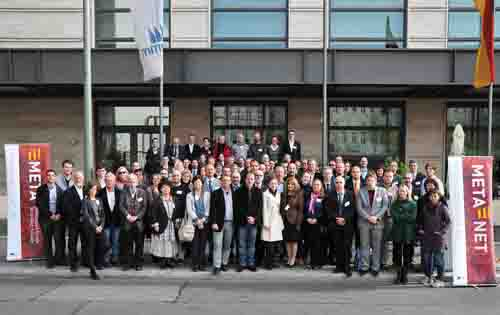
\includegraphics[width=\textwidth]{../_media/meta-net_team.jpg}
  \caption{Περίπου 100 επαγγελματίες της Γλωσικής Τεχνολογίας και εκπρόσωποι των χωρών και των γλωσσών του ΜΕΤΑ-ΝΕΤ συζήτησαν και κατέληξαν στα κύρια αποτελέσματα και μηνύματα των λευκών βίβλων κατά τη διάρκεια της συνάντησης του ΜΕΤΑ-ΝΕΤ στο Βερολίνο, στις 21/22 Οκτωβρίου 2011. --- \textcolor{grey1}{About 100 language technology experts -- representatives of the countries and languages represented in META-NET -- discussed and finalised the key results and messages of the White Paper Series at a META-NET meeting in Berlin, Germany, on October 21/22, 2011.}}
  \medskip
  \colorrule{grey3}{\textwidth}{1.5pt}
\end{figure*}

\cleardoublepage

\bsection[Σειρά Λευκών Βίβλων του META-NET -- The META-NET White Paper Series]{Σειρά Λευκών Βίβλων META-NET --- The META-NET\ \ \ \ \ \ \ White Paper Series}
\label{whitepaperseries}

\selectlanguage{english}

\vspace*{-5mm}
\centering
  \setlength{\tabcolsep}{2em}
  \begin{tabularx}{\textwidth}{lllll} \toprule\addlinespace
  &αγγλικά & English & English& \\
  &βασκικά & Basque & euskara& \\
  &βουλγαρικά & Bulgarian & български& \\
  &γαλικιανά & Galician & galego& \\
  &γαλλικά & French & français& \\
  &γερμανικά & German & Deutsch& \\
  &δανικά & Danish & dansk& \\
  &ελληνικά & Greek & ελληνικά& \\
  &εσθονικά & Estonian & eesti& \\
  &ιρλανδικά & Irish & Gaeilge& \\
  &ισλανδικά & Icelandic & íslenska& \\
  &ισπανικά & Spanish & español& \\
  &ιταλικά & Italian & italiano& \\
  &καταλανικά & Catalan & català& \\
  &κροατικά & Croatian & hrvatski& \\
  &λεττονικά & Latvian & latviešu valoda& \\
  &λιθουανικά & Lithuanian & lietuvių kalba& \\
  &μαλτέζικα & Maltese & Malti& \\
  &νορβηγικά μποκμάλ & Norwegian Bokmål & bokmål& \\
  &νορβηγικά νινόρσκ & Norwegian Nynorsk & nynorsk& \\
  &ολλανδικά & Dutch & Nederlands& \\
  &ουγγρικά & Hungarian & magyar& \\
  &πολωνικά & Polish & polski& \\
  &πορτογαλικά & Portuguese & português& \\
  &ρουμανικά & Romanian & română& \\
  &σερβικά & Serbian & српски& \\
  &σλοβακικά & Slovak & slovenčina& \\
  &σλοβενικά & Slovene & slovenščina& \\
  &σουηδικά & Swedish & svenska& \\
  &τσεχικά & Czech & čeština& \\
  &φινλανδικά & Finnish & suomi& \\ \addlinespace \bottomrule
\end{tabularx}

\end{document}
